%*****************************************
\chapter{\textbf{Gaia and SuperWASP sample data}} \label{ch: Data}
%*****************************************
\vspace{0.5cm} 
%============================================================================================================================================================

\section{Introduction}

The main goal of the project is to target young-star populations to enhance the probability of observing exoplanetary rings transiting in front of their parent star as a result of the probabilistic analysis addressed in \autoref{ch: Model}. Therefore, we mainly focused our study in the well-known OB association ScoCen which is traditionally sub-divided into three different regions: \textit{Lower Centaurus Crux} (LCC), \textit{Upper Centaurus Lupus} (UCL), and \textit{Upper Scorpius} (US). The \textit{Gaia}-DR1 and-DR2 data were used to select the final sample of stars satisfying conditions on the distance, parallaxes and proper motions based on previous research (\cauthor{2018MNRAS.tmp..210W} \citeyear{2018MNRAS.tmp..210W}; \cauthor{2016MNRAS.461..794P} \citeyear{2016MNRAS.461..794P}; \cauthor{1989A&A...216...44D} \citeyear{1989A&A...216...44D}). However, also a selection based on stellar evolution tracks and isochrones using the \textit{MESA}-code provided through the \textit{MIST}-package (\cauthor{2016ApJS..222....8D} \citeyear{2016ApJS..222....8D}; \cauthor{2016ApJ...823..102C} \citeyear{2016ApJ...823..102C}) was performed to guarantee that the final sample consists of stars between $5$Myr to $60$Myr. This information is needed in order to obtain the $RA$ and $DEC$ coordinates of the objects of interest and retrieve the available light curves using the \textit{SuperWASP}-database (\cauthor{2006PASP..118.1407P} \citeyear{2006PASP..118.1407P}; \cauthor{2010A&A...520L..10B} \citeyear{2010A&A...520L..10B}). The main results from the \textit{Gaia}-and \textit{SuperWASP}-queries are presented in more detail in the next sections, including the light-curves preliminary results which are addressed extensively in \autoref{ch: Results} .   
%============================================================================================================================================================

% \section{ScoCen OB Association}
%============================================================================================================================================================

\section{Gaia Samples}\label{sec:GaiaSamples}

The \textit{Gaia}-DR1 and-DR2 data was used to select stars which belong to the ScoCen OB association. The queries were carried out using the ADQL-query interface provided by the ESA (\url{https://gea.esac.esa.int/archive/}) and shown in \autoref{ch:Appendix} for each of the three regions conforming ScoCen i.e. LCC, UCL, and US. The approach was tested in \textit{Gaia}-DR1, but later on was extended to the new data provided by the DR2 to increase the sample of stars belonging to ScoCen, and also to increase the chance of matching a star with a light curve in the \textit{SuperWASP}-database. This will be addressed at the end. The most relevant parameters retrieved for each object are the RA and DEC coordinates, galactic longitude (l) and latitude (b), parallax, the magnitude in the G-band, color index G-Ks, and the proper motion in RA and DEC.\\    

First of all, a sample based on previous physical parameters and values obtained for this association is needed in order to constrain the sample and avoid pollution from stars which may not be part of it. Following \cauthor{2018MNRAS.tmp..210W} (\citeyear{2018MNRAS.tmp..210W}), the spatial distribution of the three regions were selected using the galactic coordinates cut reported by \cauthor{2012yCat..74163108R} (\citeyear{2012yCat..74163108R}) and \cauthor{1999AJ....117..354D} (\citeyear{1999AJ....117..354D}) as shown in \autoref{tab:ScoCen_SpatialDist}. Also in distance, using a parallax range from $6$mas to $12$mas which leads to a distance range of $\sim 83-167$pc. We decided to include a wide range in distance because ScoCen is known to lie between $\sim 100-150$pc \cauthor{2018MNRAS.tmp..210W} (\citeyear{2018MNRAS.tmp..210W}), so we can include a larger sample and rule out any outliers based on the dynamics of the cluster. The spatial distribution of our sample is shown in \autoref{fig:Projection_ScoCen}. The blue, orange, and red dots represent LCC, UCL, and US respectively. It is clear that the ScoCen association covers a wide range in galactic longitude (l) $\sim 90$-deg, and $\sim 45$-deg in galactic latitude (b). Initially each sub-region contains LCC $= 2310$, UCL $= 1759$, and US $= 1584$ stars respectively. However, as it is mentioned in \cauthor{2016MNRAS.461..794P} (\citeyear{2016MNRAS.461..794P}), each region has a characteristic range for the proper motions given by the dynamics of each individual subgroup and the whole interaction. According to their work, the three subgroups have a value of $\mu_\alpha < 10~\textnormal{mas}~\textnormal{yr}^{-1}$ and $\mu_\delta < 30~\textnormal{mas}~\textnormal{yr}^{-1}$, while for LCC, UCL, and US values of $15~\textnormal{mas}~\textnormal{yr}^{-1} < \mu < 55~\textnormal{mas}~\textnormal{yr}^{-1}$, $12~\textnormal{mas}~\textnormal{yr}^{-1} < \mu < 55~\textnormal{mas}~\textnormal{yr}^{-1}$, and $\mu < 47~\textnormal{mas}~\textnormal{yr}^{-1}$, respectively, are reported. This is better seen in \autoref{fig:Hist_ScoCen_Mamajek} where the histogram for the whole sample of stars selected in distance range are shown in colors, and each vertical dashed-line shows the above mentioned cuts for each subgroup. In the end, after this analysis, the query was performed taking into account the dynamical constraints of the cluster (see \autoref{ch:Appendix}) to provide a clean sample.\\  

\begin{table}[]
\centering
\caption{\scriptsize{ScoCen subgroups galactic coordinates selection box.}}
\label{tab:ScoCen_SpatialDist}
\begin{tabular}{lcccc}
\hline
Sub-group             & l$_{-}$ {[}deg{]} & l$_{+}$ {[}deg{]} & b$_{-}$ {[}deg{]} & b$_{+}$ {[}deg{]} \\ \hline \hline
Lower Centaurus Crux  & 285               & 313               & -10               & 16                \\
Upper Centaurus Lupus & 313               & 337               & 5                 & 31                \\
Upper Scorpius        & 337               & 360               & 7                 & 32                \\ \hline \hline
\end{tabular}
\end{table}

\begin{figure}[!ht]%
    \centering
    \subfloat{{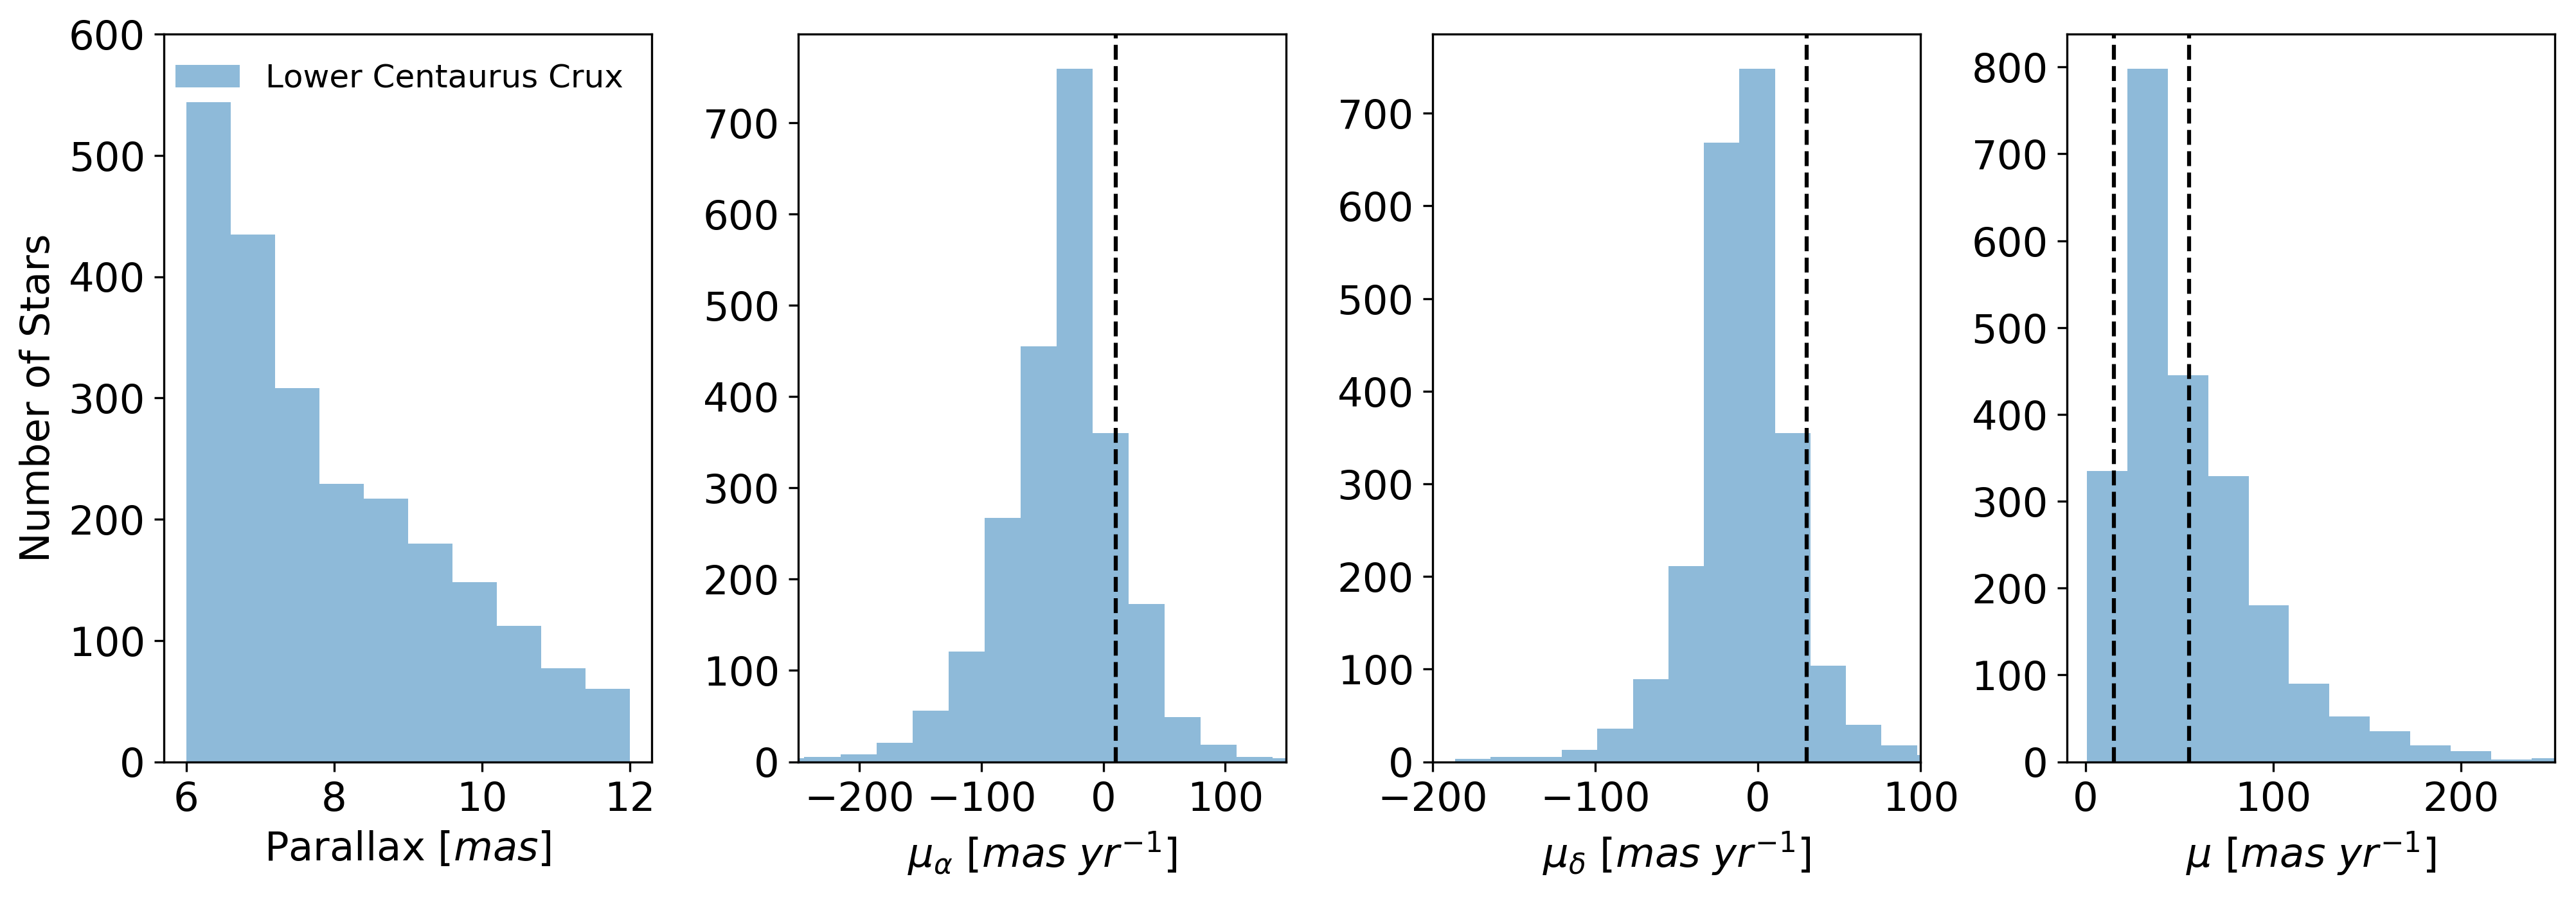
\includegraphics[width = 16cm, height = 5.5cm]{./Graficos/Capitulo_3/5_Sco-Cen/Hist_Extintion_1.png} }}%
    \qquad
    \subfloat{{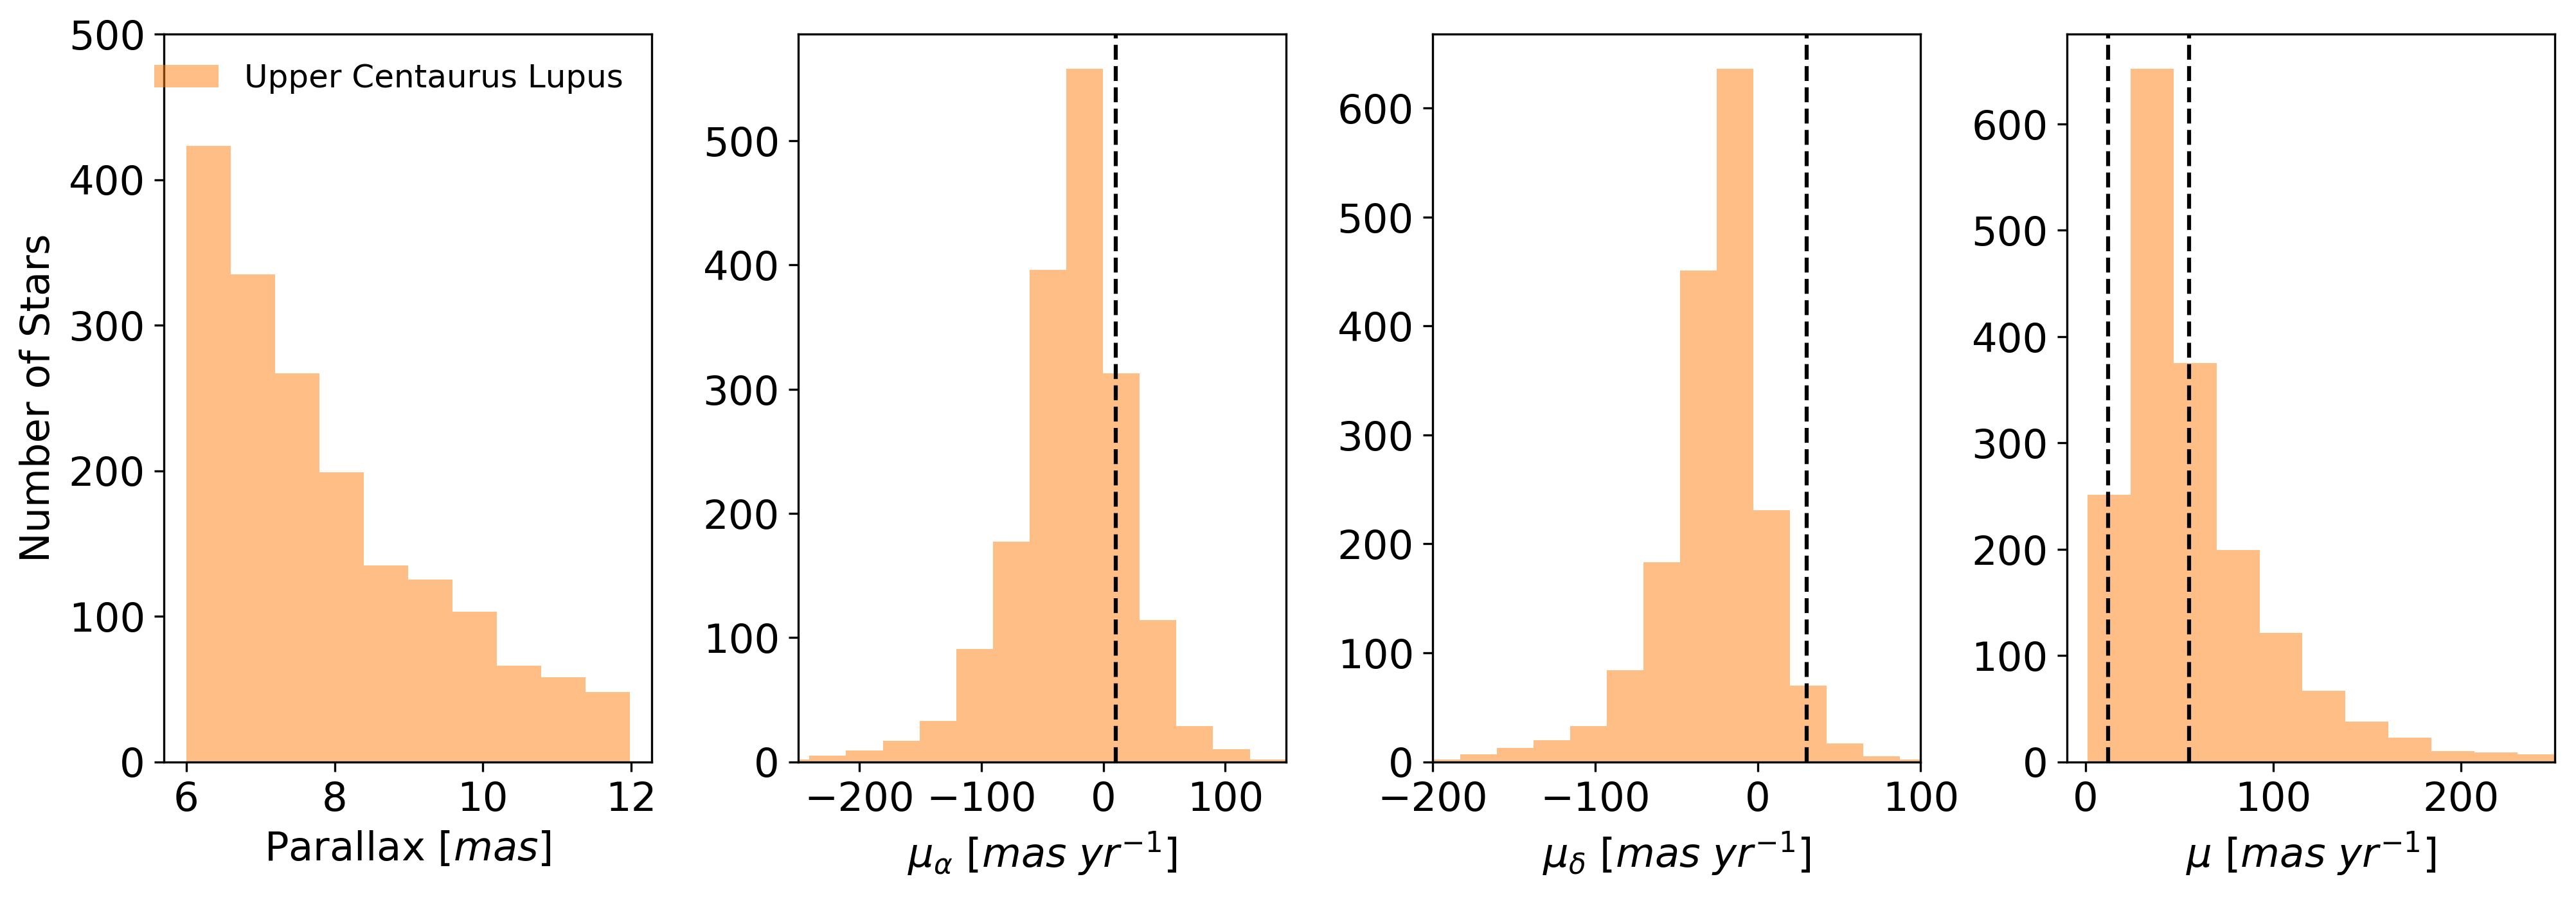
\includegraphics[width = 16cm, height = 5.5cm]{./Graficos/Capitulo_3/5_Sco-Cen/Hist_Extintion_2.png} }}%
    \qquad
    \subfloat{{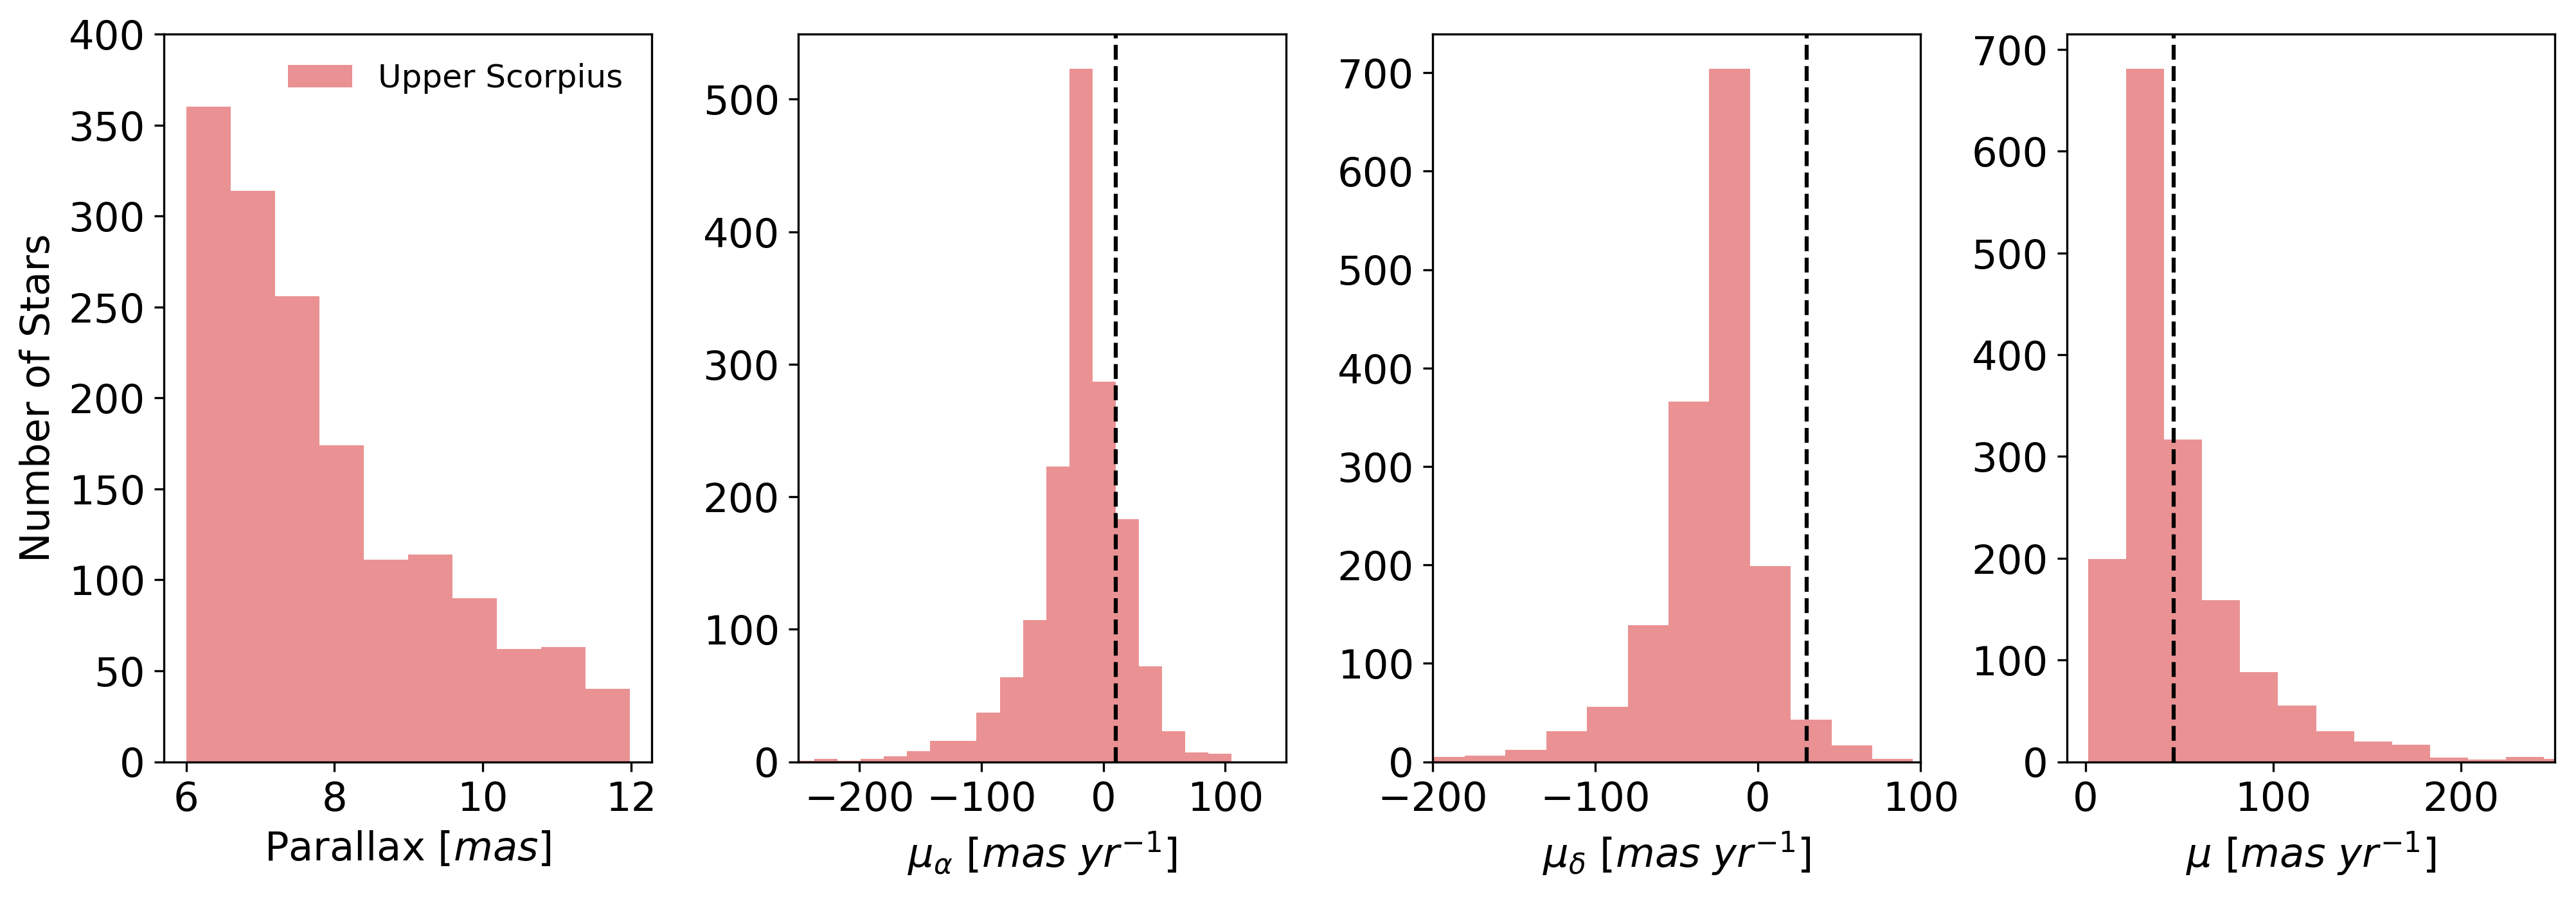
\includegraphics[width = 16cm, height = 5.5cm]{./Graficos/Capitulo_3/5_Sco-Cen/Hist_Extintion_3.png} }}%
    \caption{\scriptsize{Number of stars in LCC (blue), UCL (orange) and US (red), as a function of, from left to right, parallax, proper motion in right ascension, proper motion in declination and total proper motion. The parallax was set to satisfy ScoCen's distance range reported in literature. In the case of proper motion, cuts based on \cauthor{2018MNRAS.tmp..210W} (\citeyear{2018MNRAS.tmp..210W}) were applied, and are shown as black-dashed vertical lines.}}%
    \label{fig:Hist_ScoCen_Mamajek}%
\end{figure}  

\begin{figure}[!ht]
\centering
  \subfloat{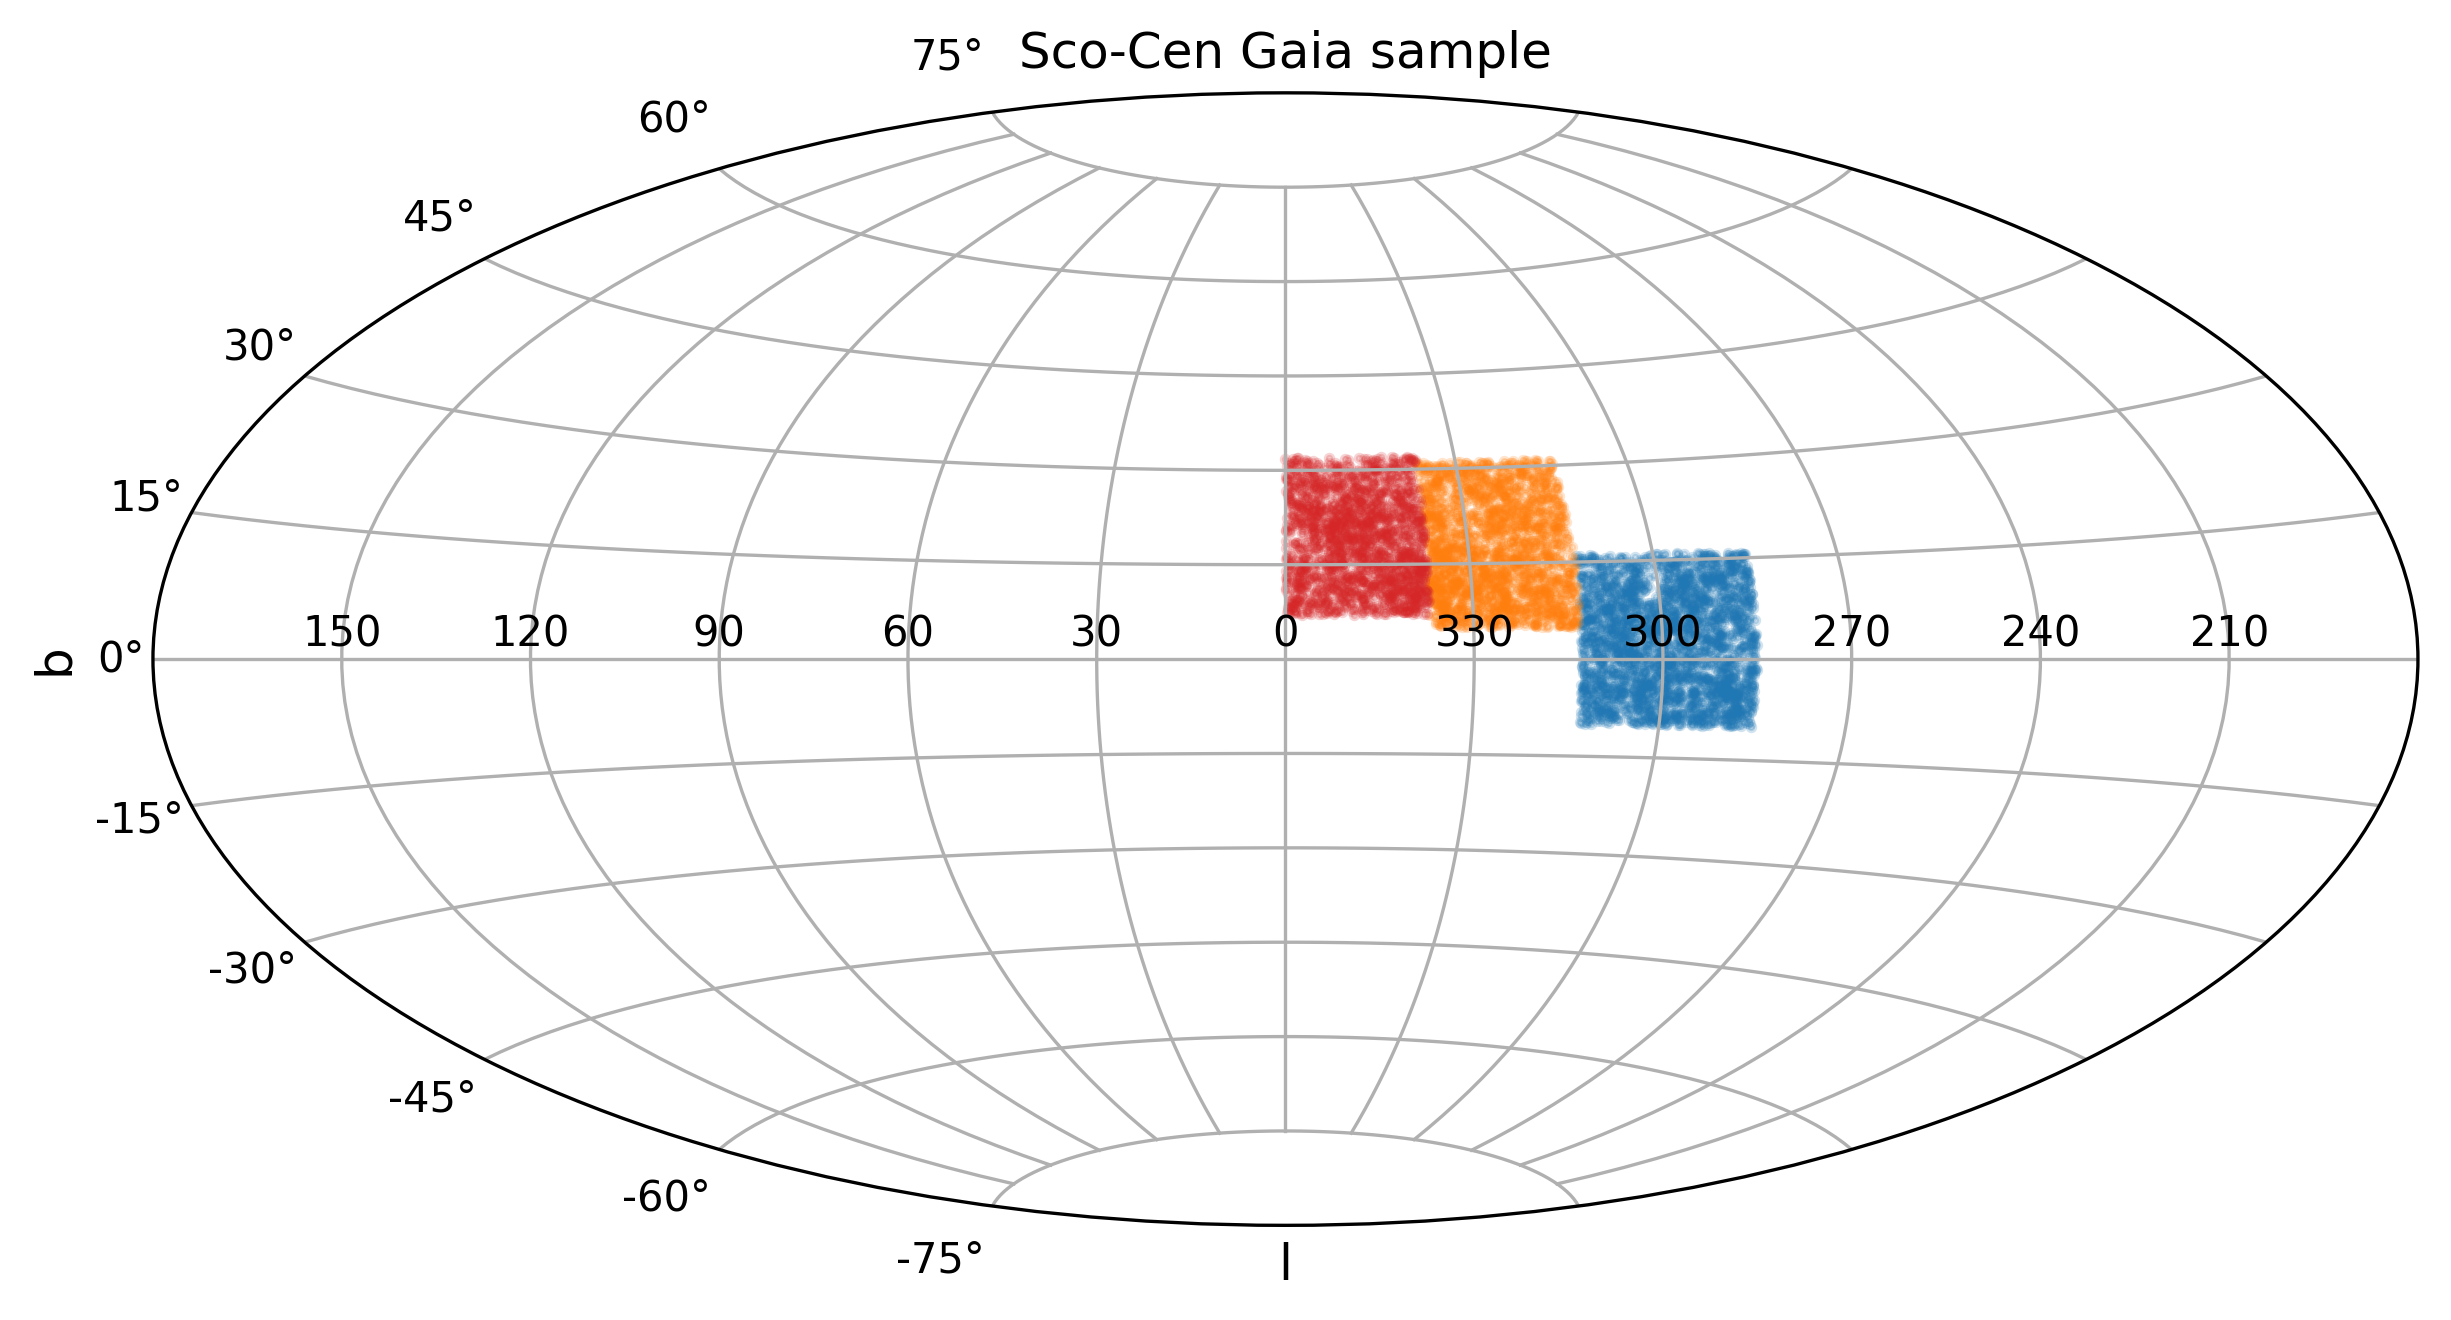
\includegraphics[width = 16cm, height = 8cm]{./Graficos/Capitulo_3/5_Sco-Cen/Sco_Cen_Projection_flipped.png}} 
\caption{\scriptsize{ScoCen subgroups position in galactic coordinates. Each subgroup LCC (blue), UCL (orange) and US (red), contains the initial sample of stars as obtained from DR1 in galactic longitude and galactic latitude. The region covers $\sim 90$-degrees in longitude and $\sim 50$-degrees in latitude.}}
\label{fig:Projection_ScoCen}
\end{figure}

This cut-off in proper motion and parallax leads to a new sample of LCC $= 1010$, UCL $= 746$, and US $= 797$ stars respectively, in which we have ruled out stars which certainly do not belong to the association. The next step is to narrow down the sample based on the stellar evolution of the cluster. This was performed using evolutionary tracks in which we aimed to use low-mass stars as they are the ones with higher probabilities of exoplanetary rings transits as shown before, and also using isochrones to restrict each sample to contain the young population. %This is thoroughly explained in \autoref{sec:SEM_1}.   


%============================================================================================================================================================

\section{Stellar Evolution Models} \label{sec:SEM_1}

The highest transit probability was obtained for low-mass stars. As shown in \autoref{fig:Rings_Prob}, the probability of detecting rings transiting in front of the parent stars decreases as the stellar mass increases independent of the lifetime for the planetary rings which only causes a vertical shift i.e. a change in the total expected number of transits. Therefore, it is important to select a reliable sample of stars in ScoCen which can lead to a high chance of detecting this kind of transits. The first step consisted in taking the sample mentioned above in which a cut-off in the dynamics and distance for the association has been applied, and run different stellar track models with an initial value of extinction $\textnormal{A}_\textnormal{v} = 0$ for each sub-region using the \textit{MIST}-package. In \autoref{fig:Stellar_Tracks_1}, the color-magnitude diagram for each sub-region is presented for $\textnormal{G}$- and $\textnormal{K}_\textnormal{s}$-bands. The magnitudes were obtained using \textit{Gaia}-DR1 and transformed to the absolute magnitude (see \autoref{ch:Appendix}). The color index was computed using a cross-match identification of the sources in \textit{Gaia}-DR1 with \textit{The Two Micron All-Sky Survey} (2MASS) tables. The stellar tracks shown correspond to stellar masses from $0.5 \textnormal{M}_\odot$ to  $2.1 \textnormal{M}_\odot$ in steps of $0.4 \textnormal{M}_\odot$, which were computed for the required photometric bands in \textit{Gaia} and \textit{2MASS}. Although each sub-region shows different spread, the stars seem to be distributed mostly below the $1.3 \textnormal{M}_\odot$ stellar track. Therefore, no-extra cut-off in mass in needed because if one compares to \autoref{fig:Rings_Prob} the highest probabilities are for stars $< 2.0 \textnormal{M}_\odot$. The same conditions were assumed to compute the isochrones shown in \autoref{fig:Isochrones_1}. Each figure corresponds to the LCC, UCL, and US color-magnitude diagrams with isochrones of $5, 15, 20, 30$ and $60$-Myr. The upper isochrone is the youngest ($5$-Myr) while the lower represents the oldest ($60$-Myr). In each of the three cases, most of the stars are contained in between the youngest and the oldest isochrones. It is useful to have in mind that all the isochrones are computed without extinction. A few stars lie outside the isochrones delimited region, thus, the idea is to use the isochrones to just select those stars that satisfy the absolute magnitude $\textnormal{M}_\textnormal{G}$ and color index $\textnormal{G} - \textnormal{K}_\textnormal{s}$ conditions in between both isochrones. After selecting only those stars in between the isochrones the final sample is reduced to LCC $= 868$, UCL $= 633$, and US $= 649$ stars respectively (see \autoref{fig:Isochrones_2} for the initial distribution of stars). For comparison in \autoref{ch:Appendix}, \autoref{sec:Sample_Selection_1}, it is shown the original sample of stars without performing the proper motion and parallax cut-off in color index versus the sample after using \cauthor{2016MNRAS.461..794P} (\citeyear{2016MNRAS.461..794P}) constraints in black-dots for each sub-region in \autoref{fig:Stellar_Tracks_1_appendix} and \autoref{fig:Isochrones_1_appendix}.\\       

\begin{figure}[!ht]
\centering
  \subfloat{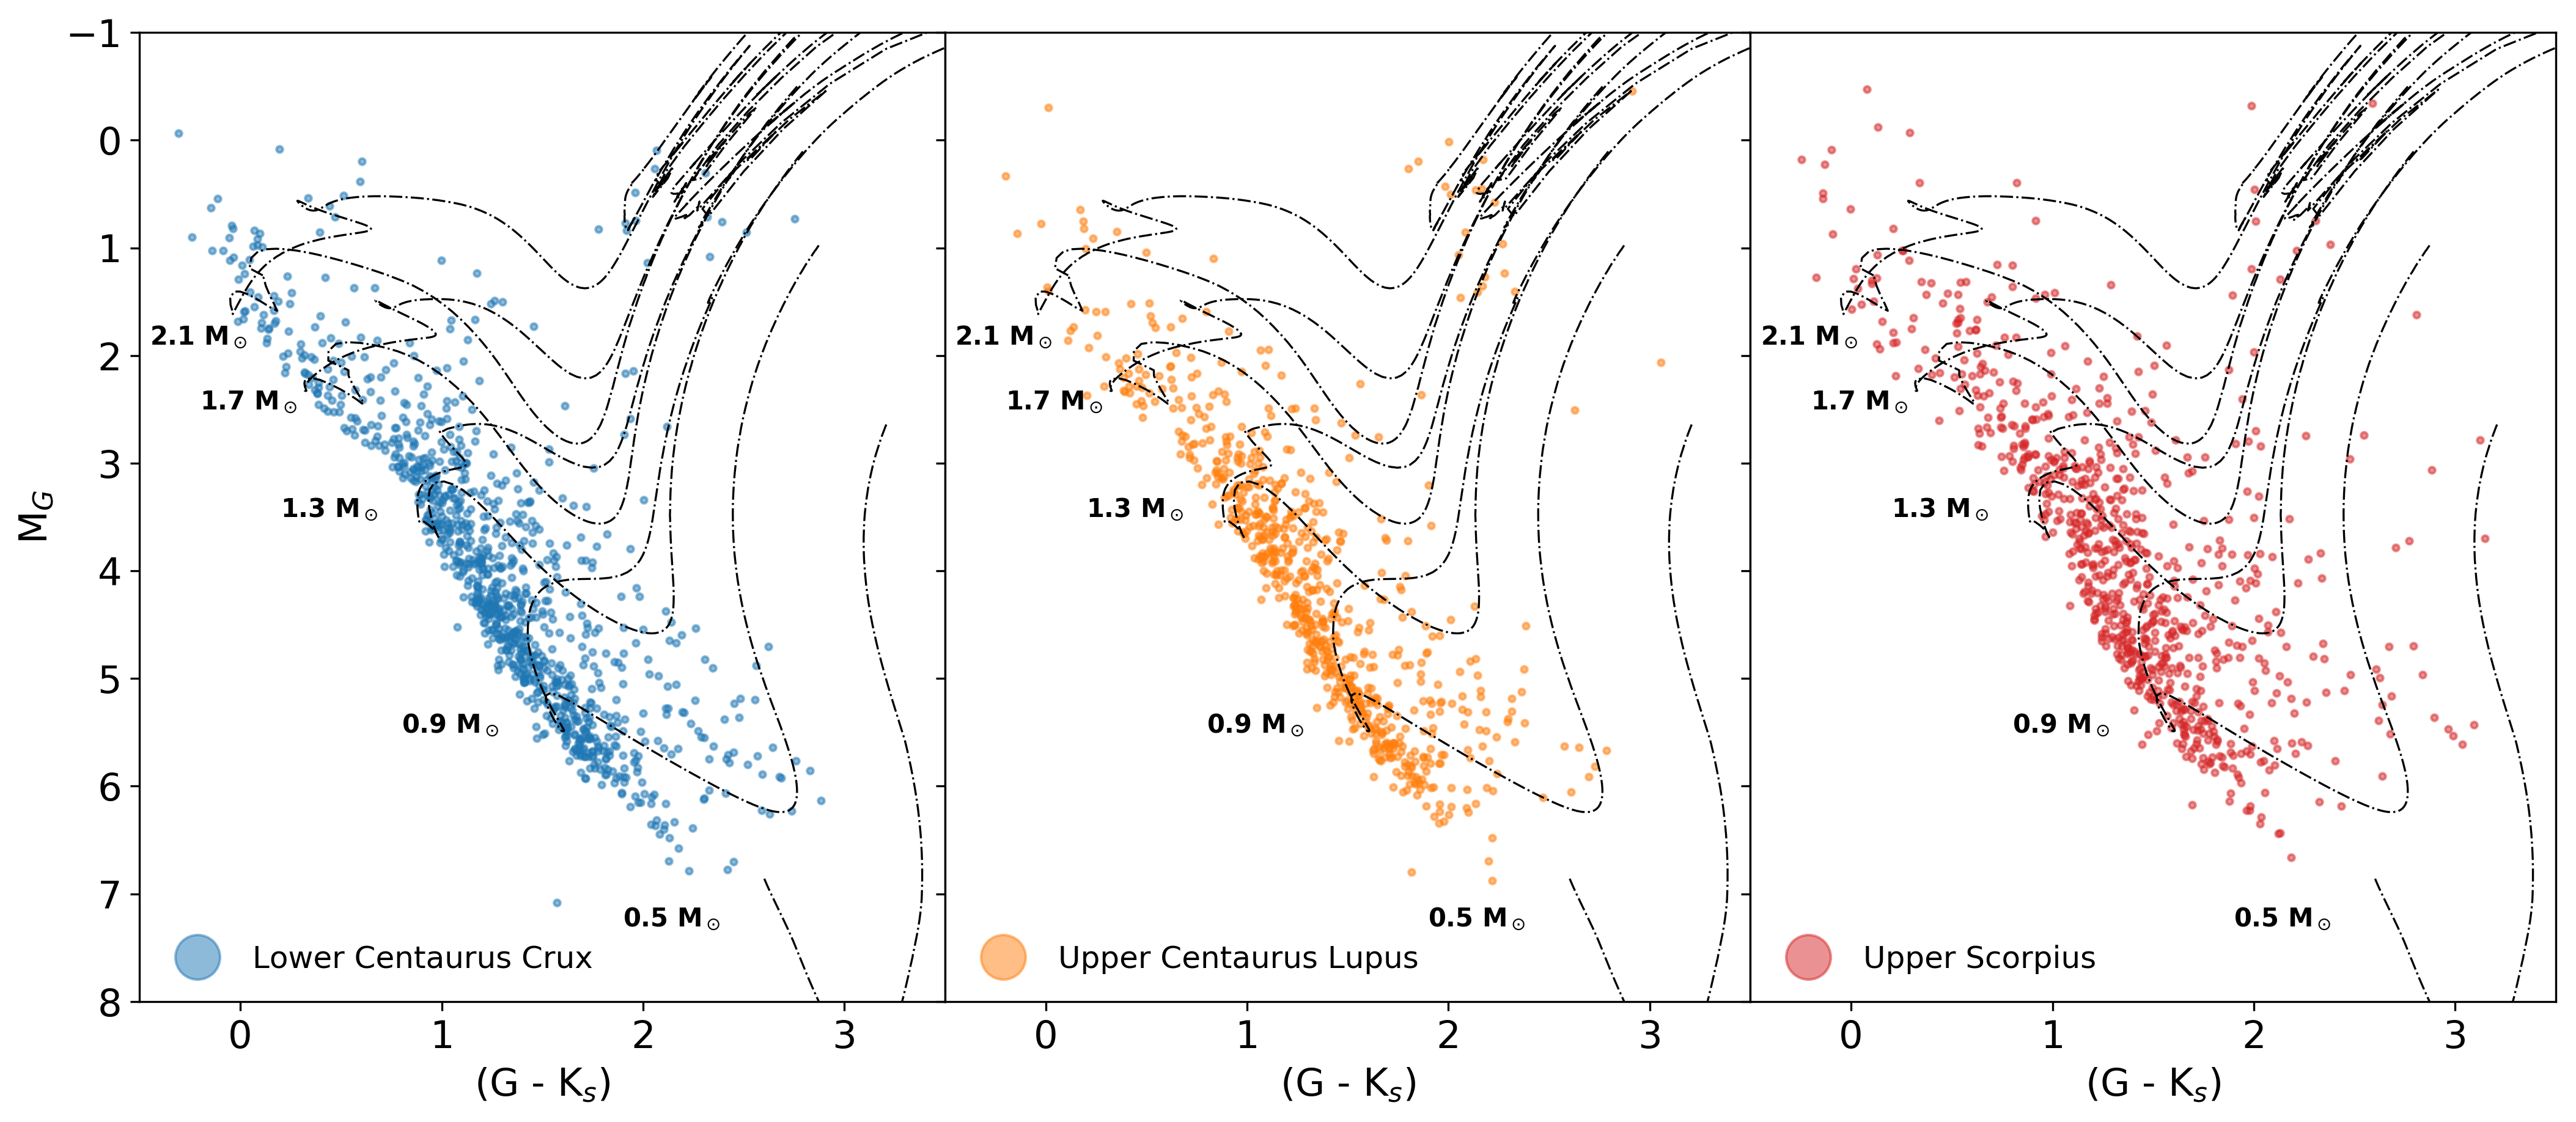
\includegraphics[width = 16cm, height = 8cm]{./Graficos/Capitulo_3/5_Sco-Cen/Mag_Col_diagram_4_2.png}} 
\caption{\scriptsize{Color-magnitude diagrams for each subgroup in ScoCen using \textit{Gaia}-DR1 data. \textit{\textbf{Left}}: LCC stars after the dynamical and positional cuts are shown in blue. The black lines correspond to different stellar tracks. \textit{\textbf{Center}}: UCL stars after the dynamical and positional cuts are shown in orange. The black lines correspond to different stellar tracks. \textit{\textbf{Right}}: US stars after the dynamical and positional cuts are shown in red. The black lines correspond to different stellar tracks. In general for each subgroup, a stellar mass range of $0.5 \textnormal{M}_\odot < \textnormal{M} < 2.1 \textnormal{M}_\odot$ was used along with $\textnormal{A}_\textnormal{v} = 0$ using the \textit{MIST}-package (\cauthor{2016ApJS..222....8D} \citeyear{2016ApJS..222....8D}; \cauthor{2016ApJ...823..102C} \citeyear{2016ApJ...823..102C}).}}
\label{fig:Stellar_Tracks_1}
\end{figure}

\begin{figure}[!ht]
\centering
  \subfloat{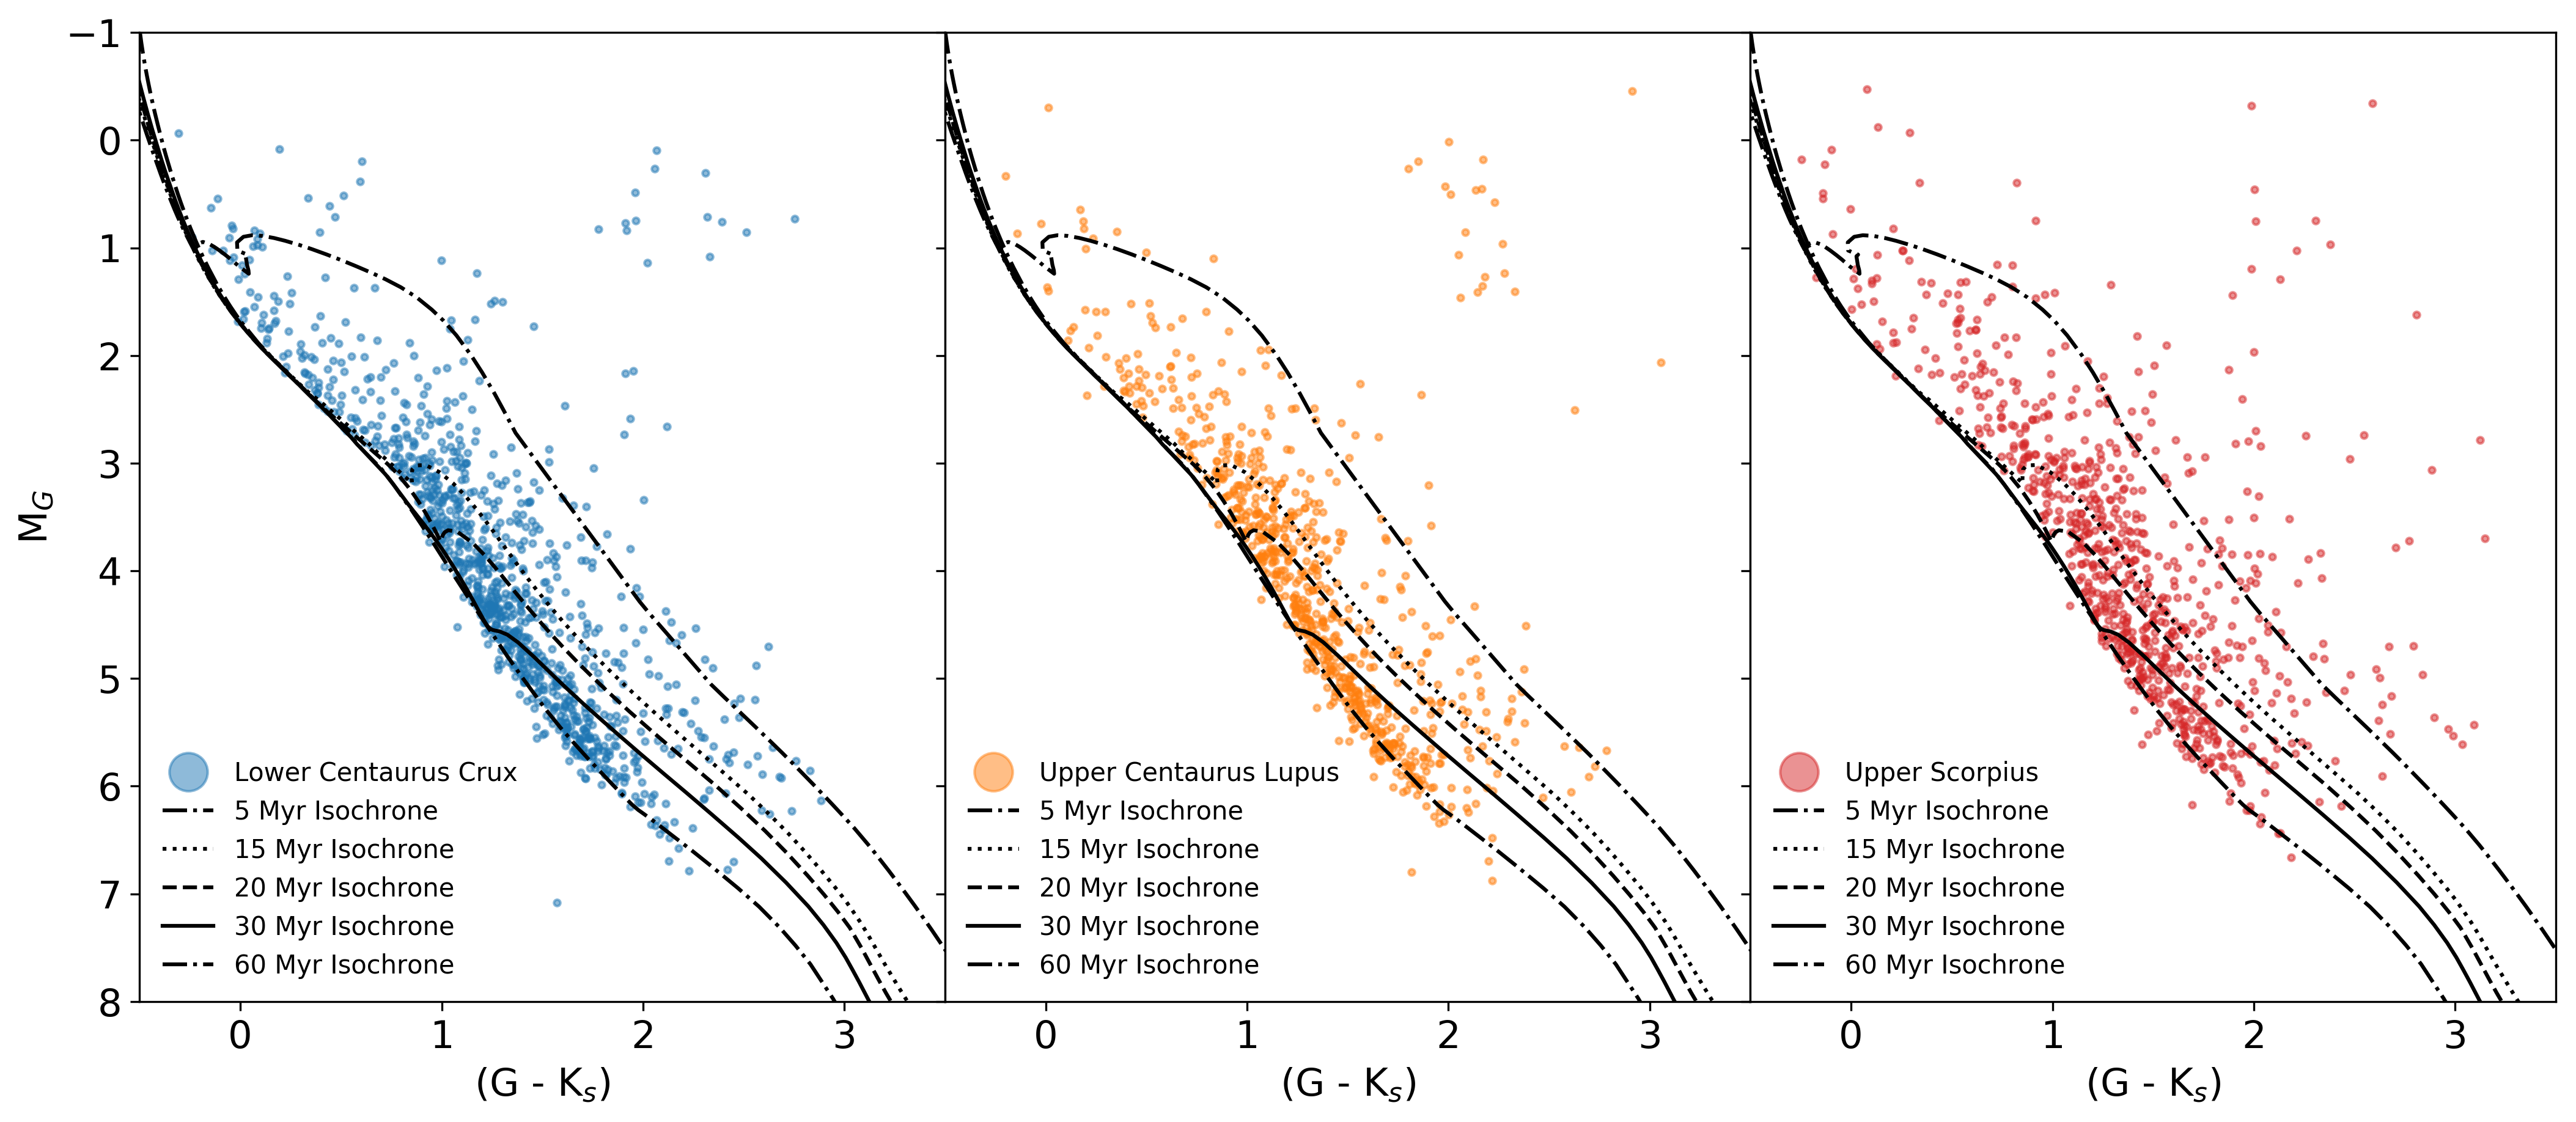
\includegraphics[width = 16cm, height = 8cm]{./Graficos/Capitulo_3/5_Sco-Cen/Mag_Col_diagram_3_Extintion_cut.png}} 
\caption{\scriptsize{Color-magnitude diagrams for each subgroup in ScoCen using \textit{Gaia}-DR1 data. \textit{\textbf{Left}}: LCC stars after the dynamical and positional cuts are shown in blue. The black lines correspond to different isochrones. \textit{\textbf{Center}}: UCL stars after the dynamical and positional cuts are shown in orange. The black lines correspond to different isochrones. \textit{\textbf{Right}}: US stars after the dynamical and positional cuts are shown in red. The black lines correspond to different isochrones. In general for each subgroup, isochrones from $5 \textnormal{Myr}$ to $60 \textnormal{Myr}$ were calculated along with $\textnormal{A}_\textnormal{v} = 0$ using the \textit{MIST}-package (\cauthor{2016ApJS..222....8D} \citeyear{2016ApJS..222....8D}; \cauthor{2016ApJ...823..102C} \citeyear{2016ApJ...823..102C}). The $60 \textnormal{Myr}$ isochrone fits well the main-sequence and the $5 \textnormal{Myr}$ isochrones gives a good range to pre-select young stars.}}
\label{fig:Isochrones_1}
\end{figure}

% \begin{figure}[!ht]
% \centering
%   \subfloat{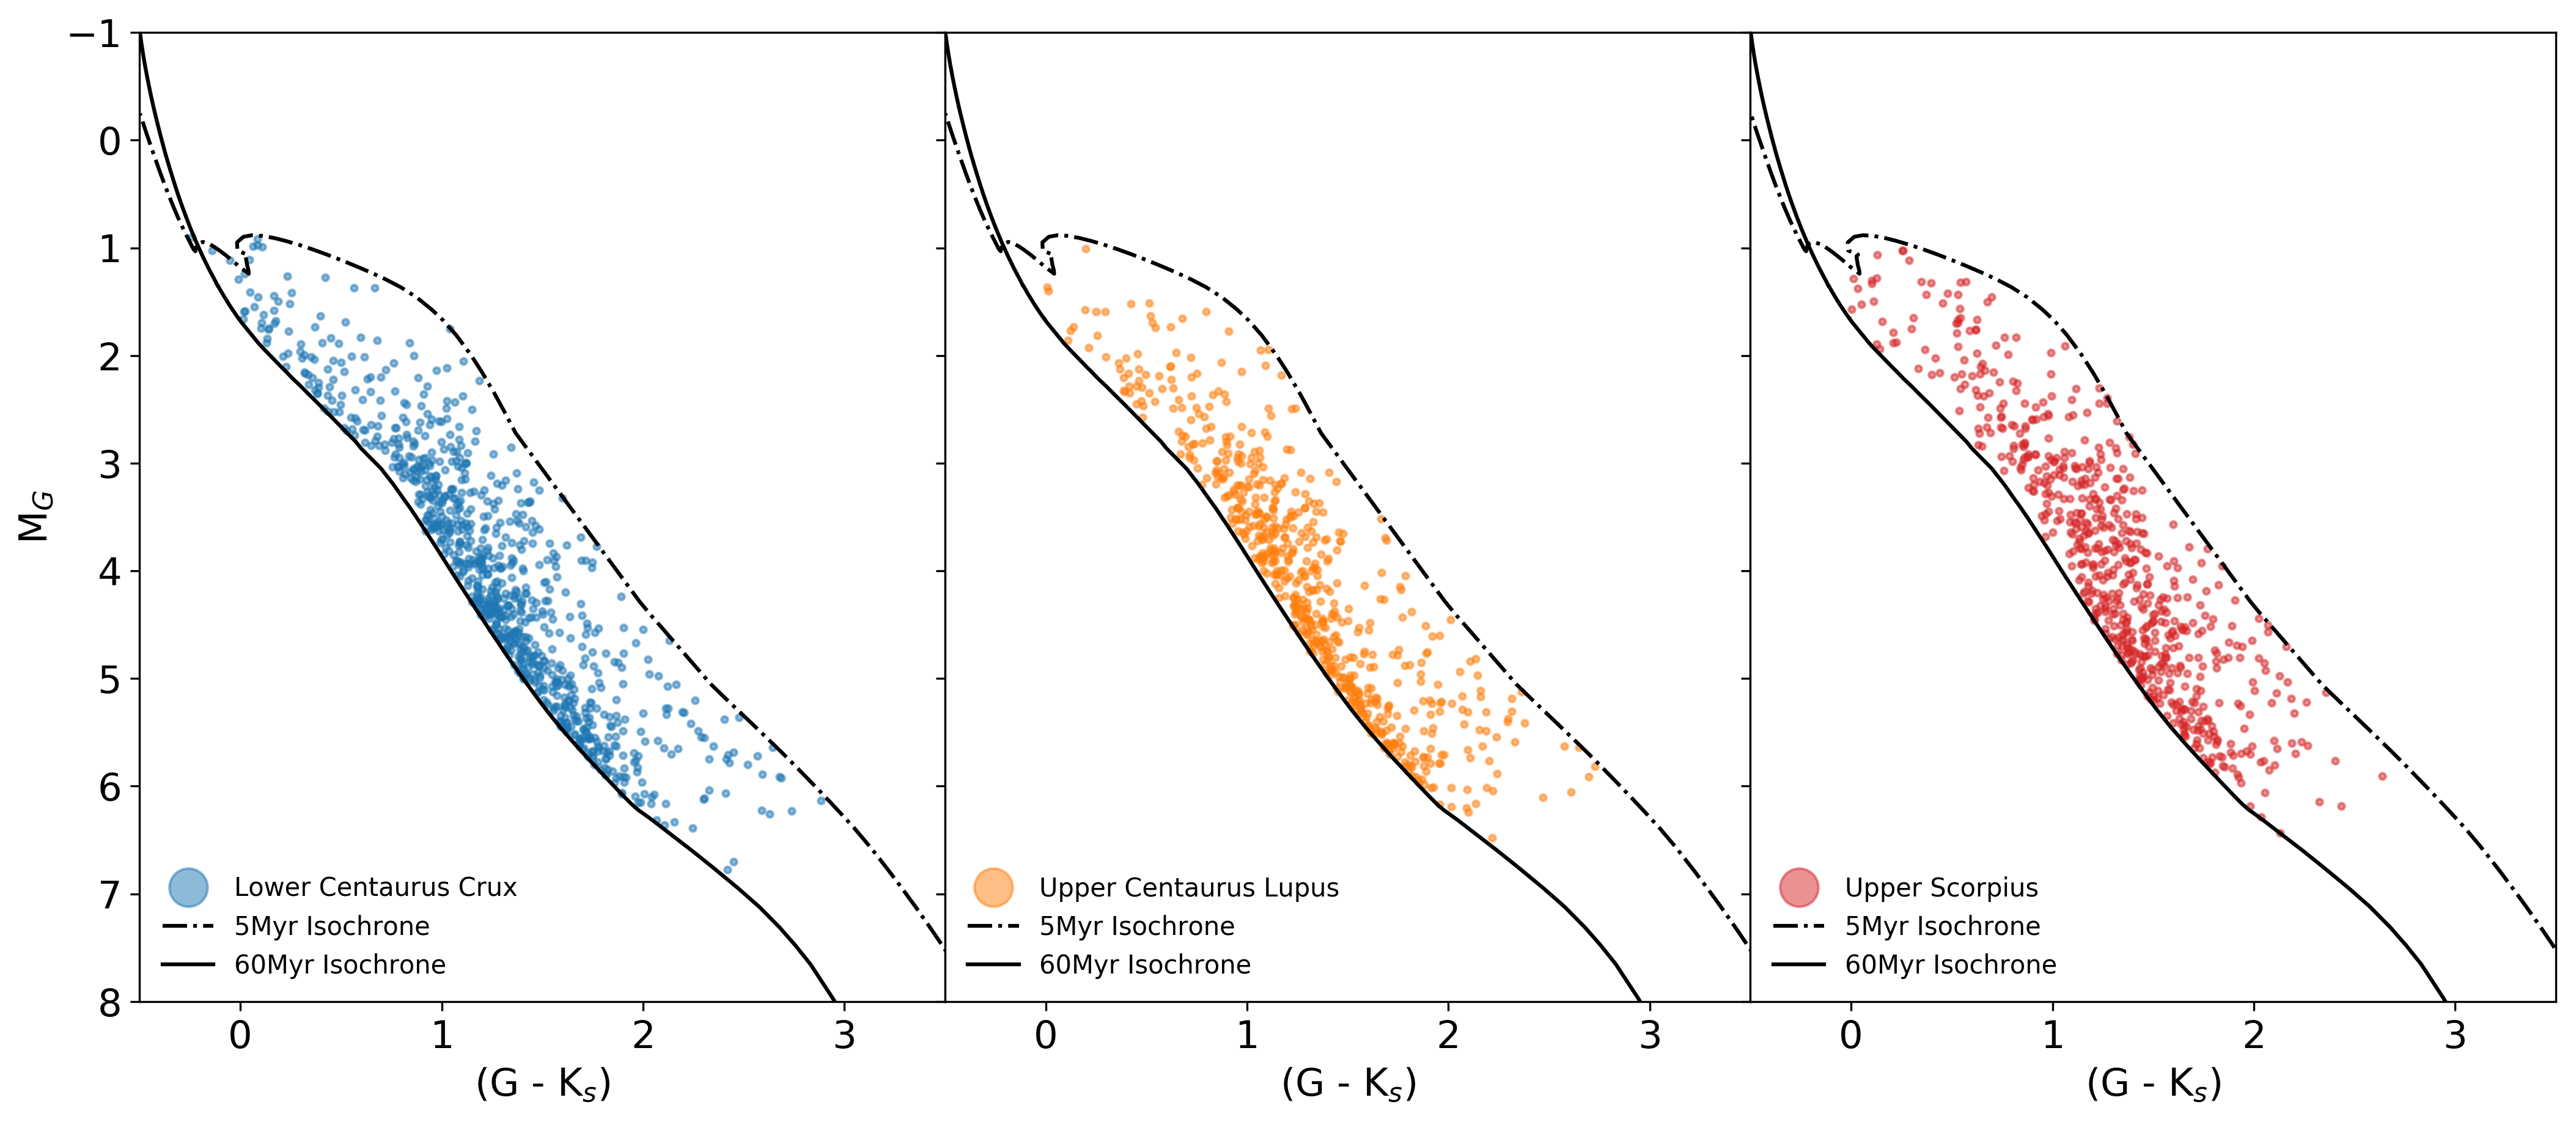
\includegraphics[width = 16cm, height = 8cm]{./Graficos/Capitulo_3/5_Sco-Cen/final_Sample_SCOCEN_Original.png}} 
% \caption{\scriptsize{Color-magnitude diagrams for each subgroup in ScoCen using selected \textit{Gaia}-DR1 data between two different isochrones. \textit{Left}: LCC stars after the dynamical and positional cuts are shown in blue. The black lines correspond to different isochrones. \textit{Center}: UCL stars after the dynamical and positional cuts are shown in orange. The black lines correspond to different isochrones. \textit{Right}: US stars after the dynamical and positional cuts are shown in red. The black lines correspond to different isochrones. Only the $5 \textnormal{Myr}$ to $60 \textnormal{Myr}$ isochrones were used with $\textnormal{A}_\textnormal{v} = 0$ to restrict the sample of stars to be inside this particular region. Following this, stars inside the region are quite likely to belong to the cluster and be in an stellar age range suitable for our study.}}
% \label{fig:Isochrones_2}
% \end{figure}

Besides this, if we want to obtain a reliable sample of stars which belong to ScoCen, we need to include the extinction in each sub-region when computing the stellar tracks and isochrones. As can be seen from \autoref{fig:Isochrones_1}, the $60$-Myr gently touches the main-sequence of this association, thus, it seems legit to compute this isochrone with $\textnormal{A}_\textnormal{v} = 0$ because extinction will shift the isochrones downwards and to the red side of the Hertzsprung-Russell diagram where stars appear fainter and redder. However, in the case of the $5$-Myr isochrone, if we include extinction, then the isochrone will shift upwards including more stars that could be ruled out by our first selection method. Therefore, we proceed to compute the $5$-Myr isochrone including the extinction factor. Based on observations made by \cauthor{1989A&A...216...44D} (\citeyear{1989A&A...216...44D}), we were able to calculate the average, median and $90$-percentile extinction values for each sub-region. In the case of LCC, a total number of 41 stars were used, while for UCL and US, 141 and 100 stars, respectively. In \autoref{fig:SCOCEN_Extinction}, the histograms for each sub-region are shown along with the average, median, and $90$-percentile extinction values. In the case of LCC and UCL, the values are always quite similar, but in the case of US, the values are significantly higher which may affect more drastically the isochrones and stellar tracks in comparison to the other two sub-regions. The values obtained for the average, are in agreement with values reported by \cauthor{2018MNRAS.tmp..210W} (\citeyear{2018MNRAS.tmp..210W}) and are well correlated with the distribution of the dust, as seen in the IRAS $100 \mu \textnormal{m}$ map \cauthor{1989A&A...216...44D} (\citeyear{1989A&A...216...44D}). These values are $0.23$, $0.17$, and $0.76$ for LCC, UCL, and US, respectively.\\     

\begin{figure}[!ht]
\centering
  \subfloat{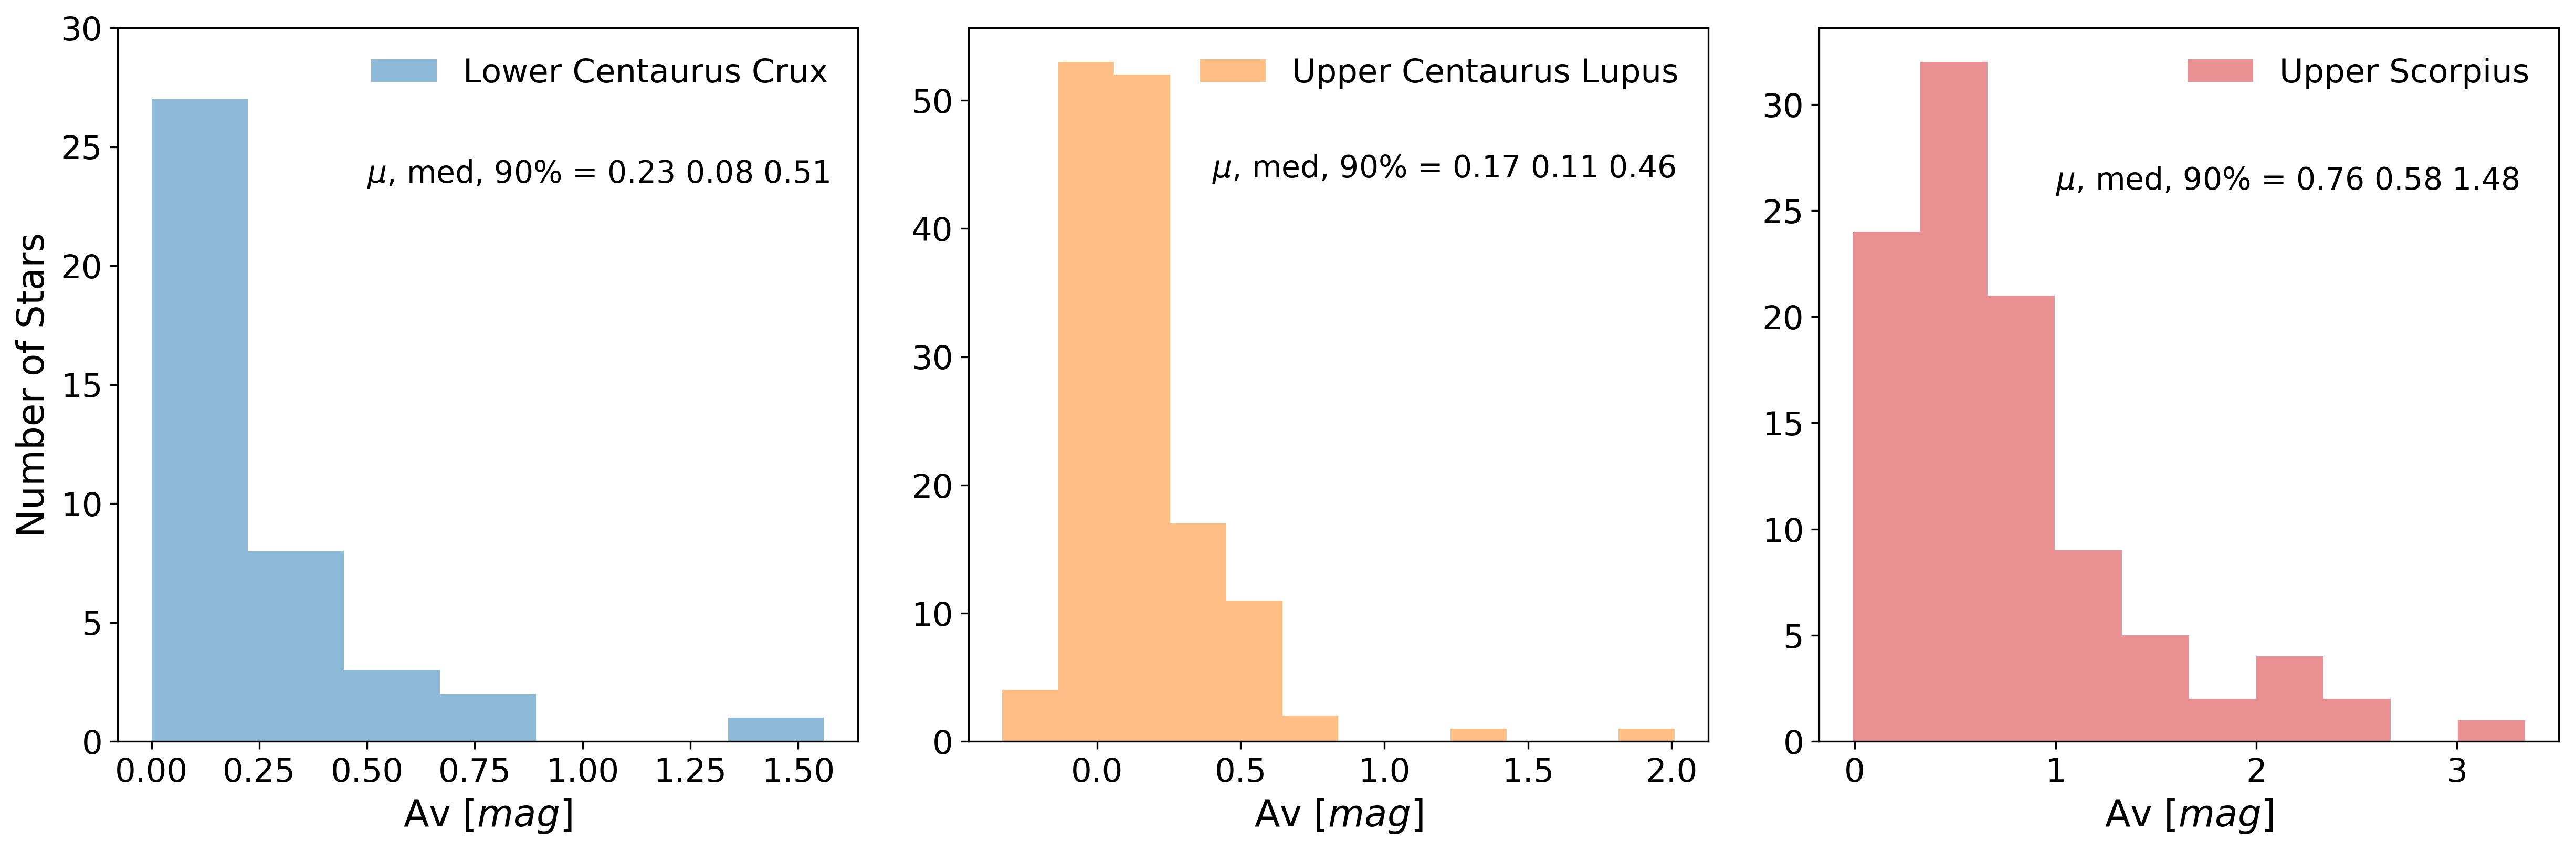
\includegraphics[width = 15.5cm, height = 5.5cm]{./Graficos/Capitulo_3/5_Sco-Cen/Av_histograms.png}} 
\caption{\scriptsize{Histograms corresponding to the number of stars as a function of extinction for each subgroup in ScoCen. Each one of the subgroups LCC, UCL, and US, contains a sample of stars reported in \cauthor{1989A&A...216...44D} (\citeyear{1989A&A...216...44D}) with measured extinction. The mean, median, and $90\%$-percentile are shown. \textit{Upper Scorpius} has the highest extinction value, while \textit{Lower Centaurus-Crux} and \textit{Upper Centaurus-Lupus} both have close extinction values.}}
\label{fig:SCOCEN_Extinction}
\end{figure}

On top of that, the $5$-Myr isochrone was computed using the average extinction values reported above to perform the selection of stars in the color-magnitude diagrams once more. As can be seen in \autoref{fig:Isochrones_3}, the shape of the $5$-Myr isochrone when introducing the extinction factor changes dramatically, increasing the number of stars affected by extintion in our selection i.e. redder and fainter ones. The same happens to LCC and UCL but in a less proportion. However, it is worth noting that the isochrones do not cross each other around $\textnormal{M}_\textnormal{G} \sim 1.0~[\textnormal{mag}]$ as was the case shown in \autoref{fig:Isochrones_1}, allowing for brighter stars to be selected in our sample. If we center our view in the stellar tracks, it is evident from \autoref{fig:Stellar_Tracks_3} that there exists a displacement downwards. However, as stars above $2.1 \textnormal{M}_\odot$ are not a lot, and this does not change that much, we will not perform any cut in stellar mass but we will just cut in stellar age using the isochrones. The new cut and final sample using the isochrones in which the youngest isochrone is affected by extinction is shown in \autoref{fig:Isochrones_4}.\\ 

\begin{figure}[!ht]
\centering
  \subfloat{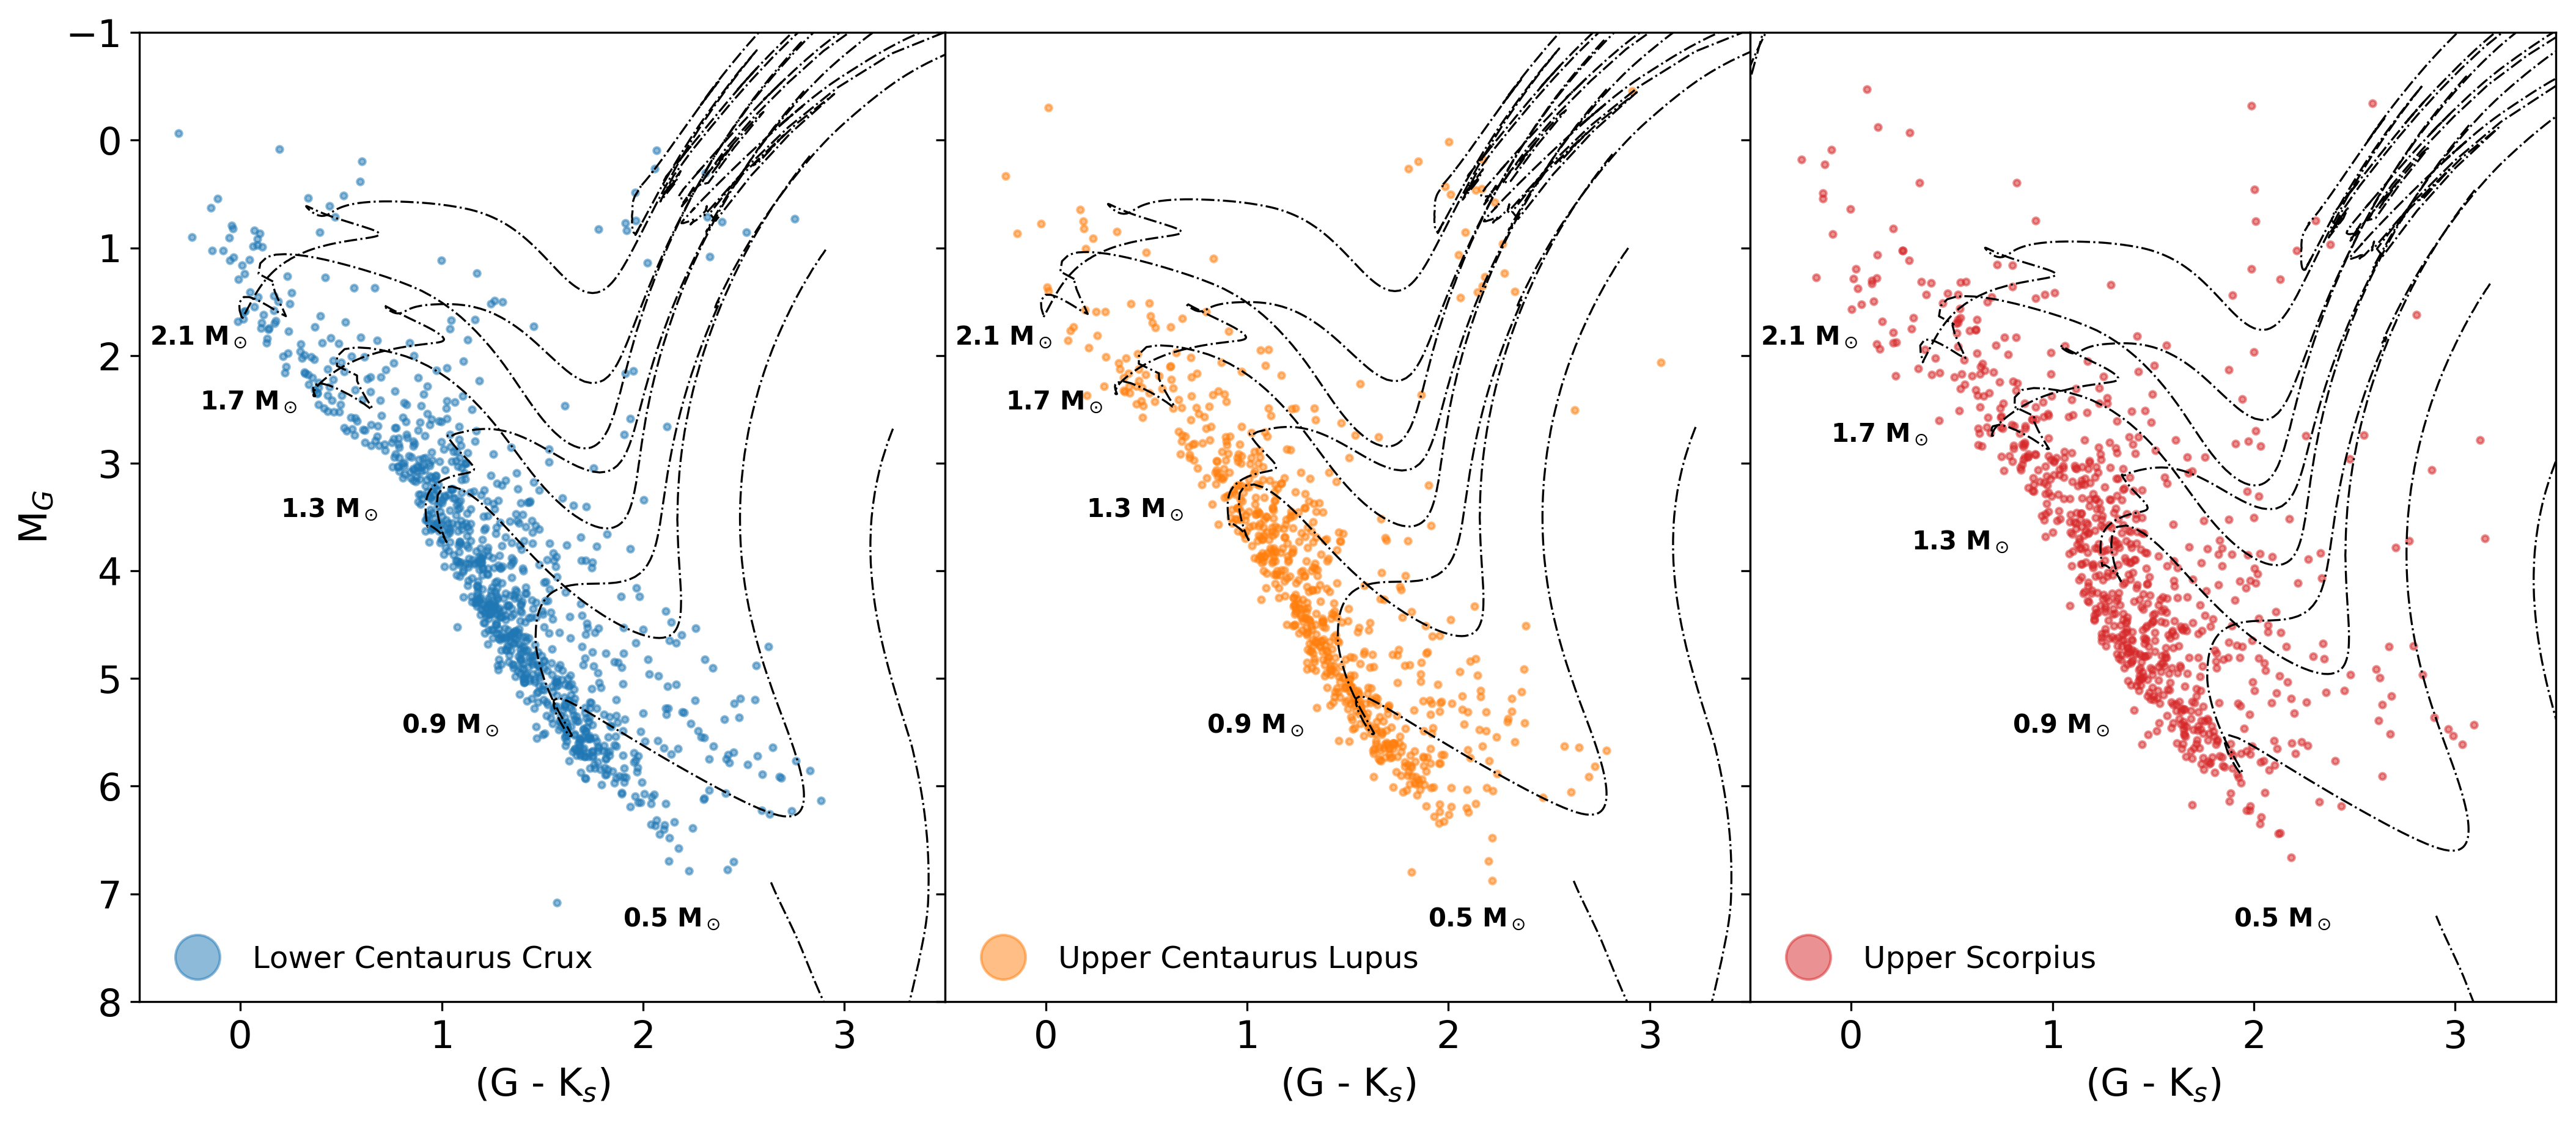
\includegraphics[width = 16cm, height = 8cm]{./Graficos/Capitulo_3/5_Sco-Cen/Mag_Col_diagram_4_Extintion_1.png}} 
\caption{\scriptsize{Color-magnitude diagrams for each subgroup in ScoCen using \textit{Gaia}-DR1 data as in \autoref{fig:Stellar_Tracks_1}, along with stellar tracks using the extinction value measured proposed by \cauthor{1989A&A...216...44D} (\citeyear{1989A&A...216...44D}). \textit{\textbf{Left}}: LCC stars after the dynamical and positional cuts are shown in blue. The black lines correspond to different stellar tracks. \textit{\textbf{Center}}: UCL stars after the dynamical and positional cuts are shown in orange. The black lines correspond to different stellar tracks. \textit{\textbf{Right}}: US stars after the dynamical and positional cuts are shown in red. The black lines correspond to different stellar tracks. In general for each subgroup, a stellar mass range of $0.5 \textnormal{M}_\odot < \textnormal{M} < 2.1 \textnormal{M}_\odot$ was used to compute the stellar tracks using the \textit{MIST}-package (\cauthor{2016ApJS..222....8D} \citeyear{2016ApJS..222....8D}; \cauthor{2016ApJ...823..102C} \citeyear{2016ApJ...823..102C}). In this case, the extinction values for LCC, UCL, and US correspond to $\textnormal{A}_\textnormal{v} = 0.23$, $\textnormal{A}_\textnormal{v} = 0.17$, and $\textnormal{A}_\textnormal{v} = 0.76$, respectively.}}
\label{fig:Stellar_Tracks_3}
\end{figure}

\begin{figure}[!ht]
\centering
  \subfloat{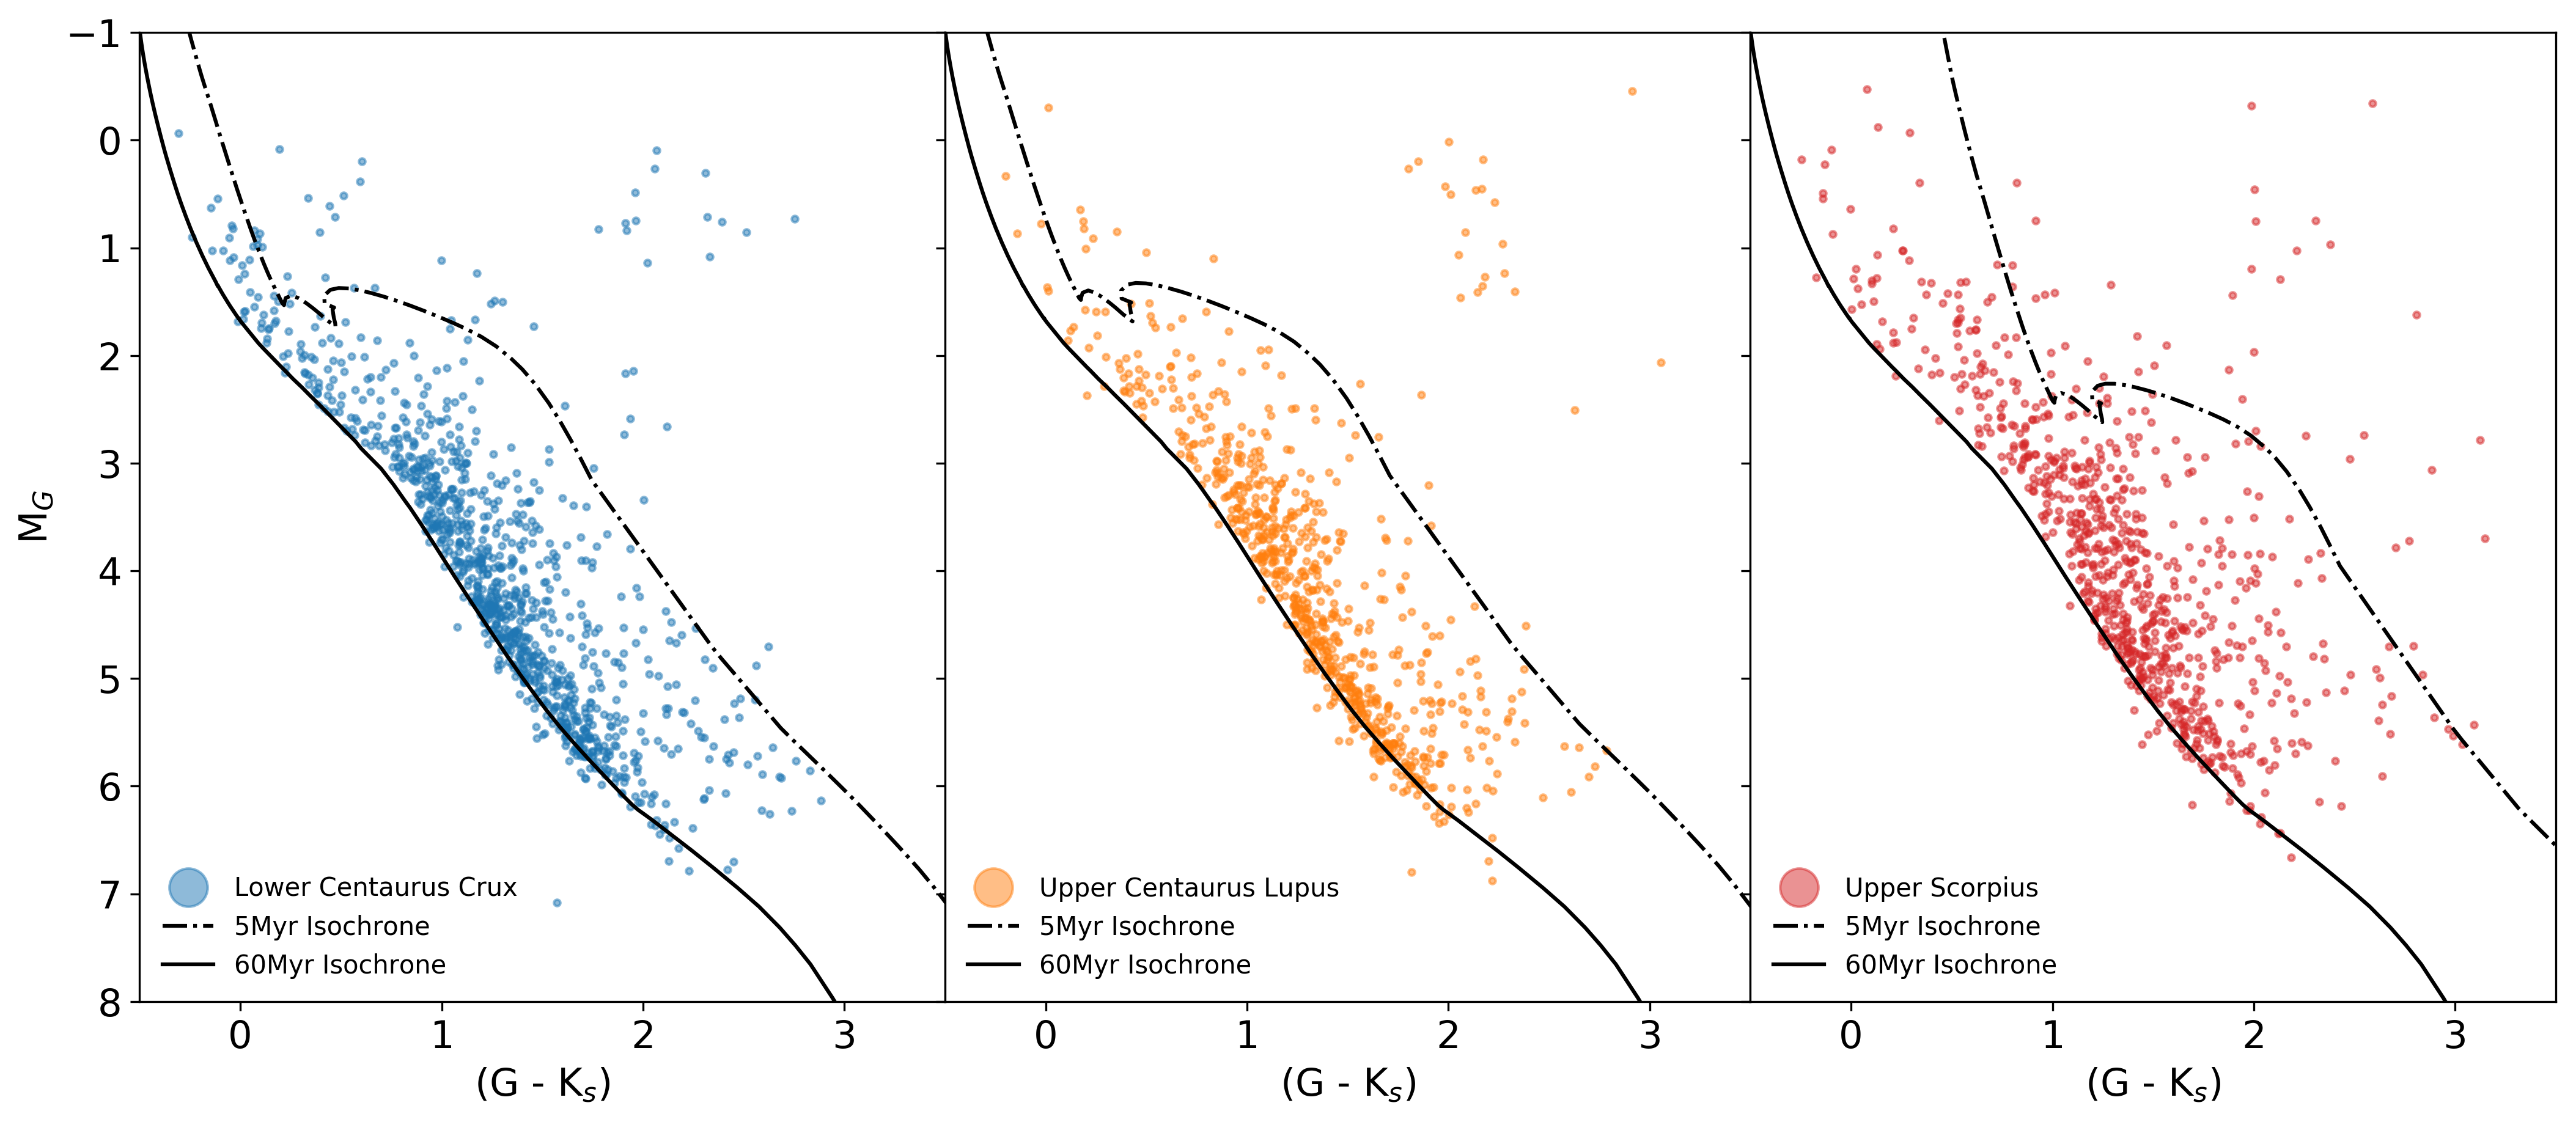
\includegraphics[width = 16cm, height = 8cm]{./Graficos/Capitulo_3/5_Sco-Cen/final_Sample_SCOCEN_2.png}} 
\caption{\scriptsize{Color-magnitude diagrams for each subgroup in ScoCen using \textit{Gaia}-DR1 data as in \autoref{fig:Isochrones_1}, along with isochrones using the extinction value measured proposed by \cauthor{1989A&A...216...44D} (\citeyear{1989A&A...216...44D}). \textit{\textbf{Left}}: LCC stars after the dynamical and positional cuts are shown in blue. The black lines correspond to different isochrones. \textit{\textbf{Center}}: UCL stars after the dynamical and positional cuts are shown in orange. The black lines correspond to different isochrones. \textit{\textbf{Right}}: US stars after the dynamical and positional cuts are shown in red. The black lines correspond to different isochrones. In general for each subgroup, two isochrones $5 \textnormal{Myr}$ and $60 \textnormal{Myr}$ were calculated using the \textit{MIST}-package (\cauthor{2016ApJS..222....8D} \citeyear{2016ApJS..222....8D}; \cauthor{2016ApJ...823..102C} \citeyear{2016ApJ...823..102C}). In this case, the extinction values for LCC, UCL, and US correspond to $\textnormal{A}_\textnormal{v} = 0.23$, $\textnormal{A}_\textnormal{v} = 0.17$, and $\textnormal{A}_\textnormal{v} = 0.76$, respectively.}}
\label{fig:Isochrones_3}
\end{figure}

% \begin{figure}[!ht]
% \centering
%   \subfloat{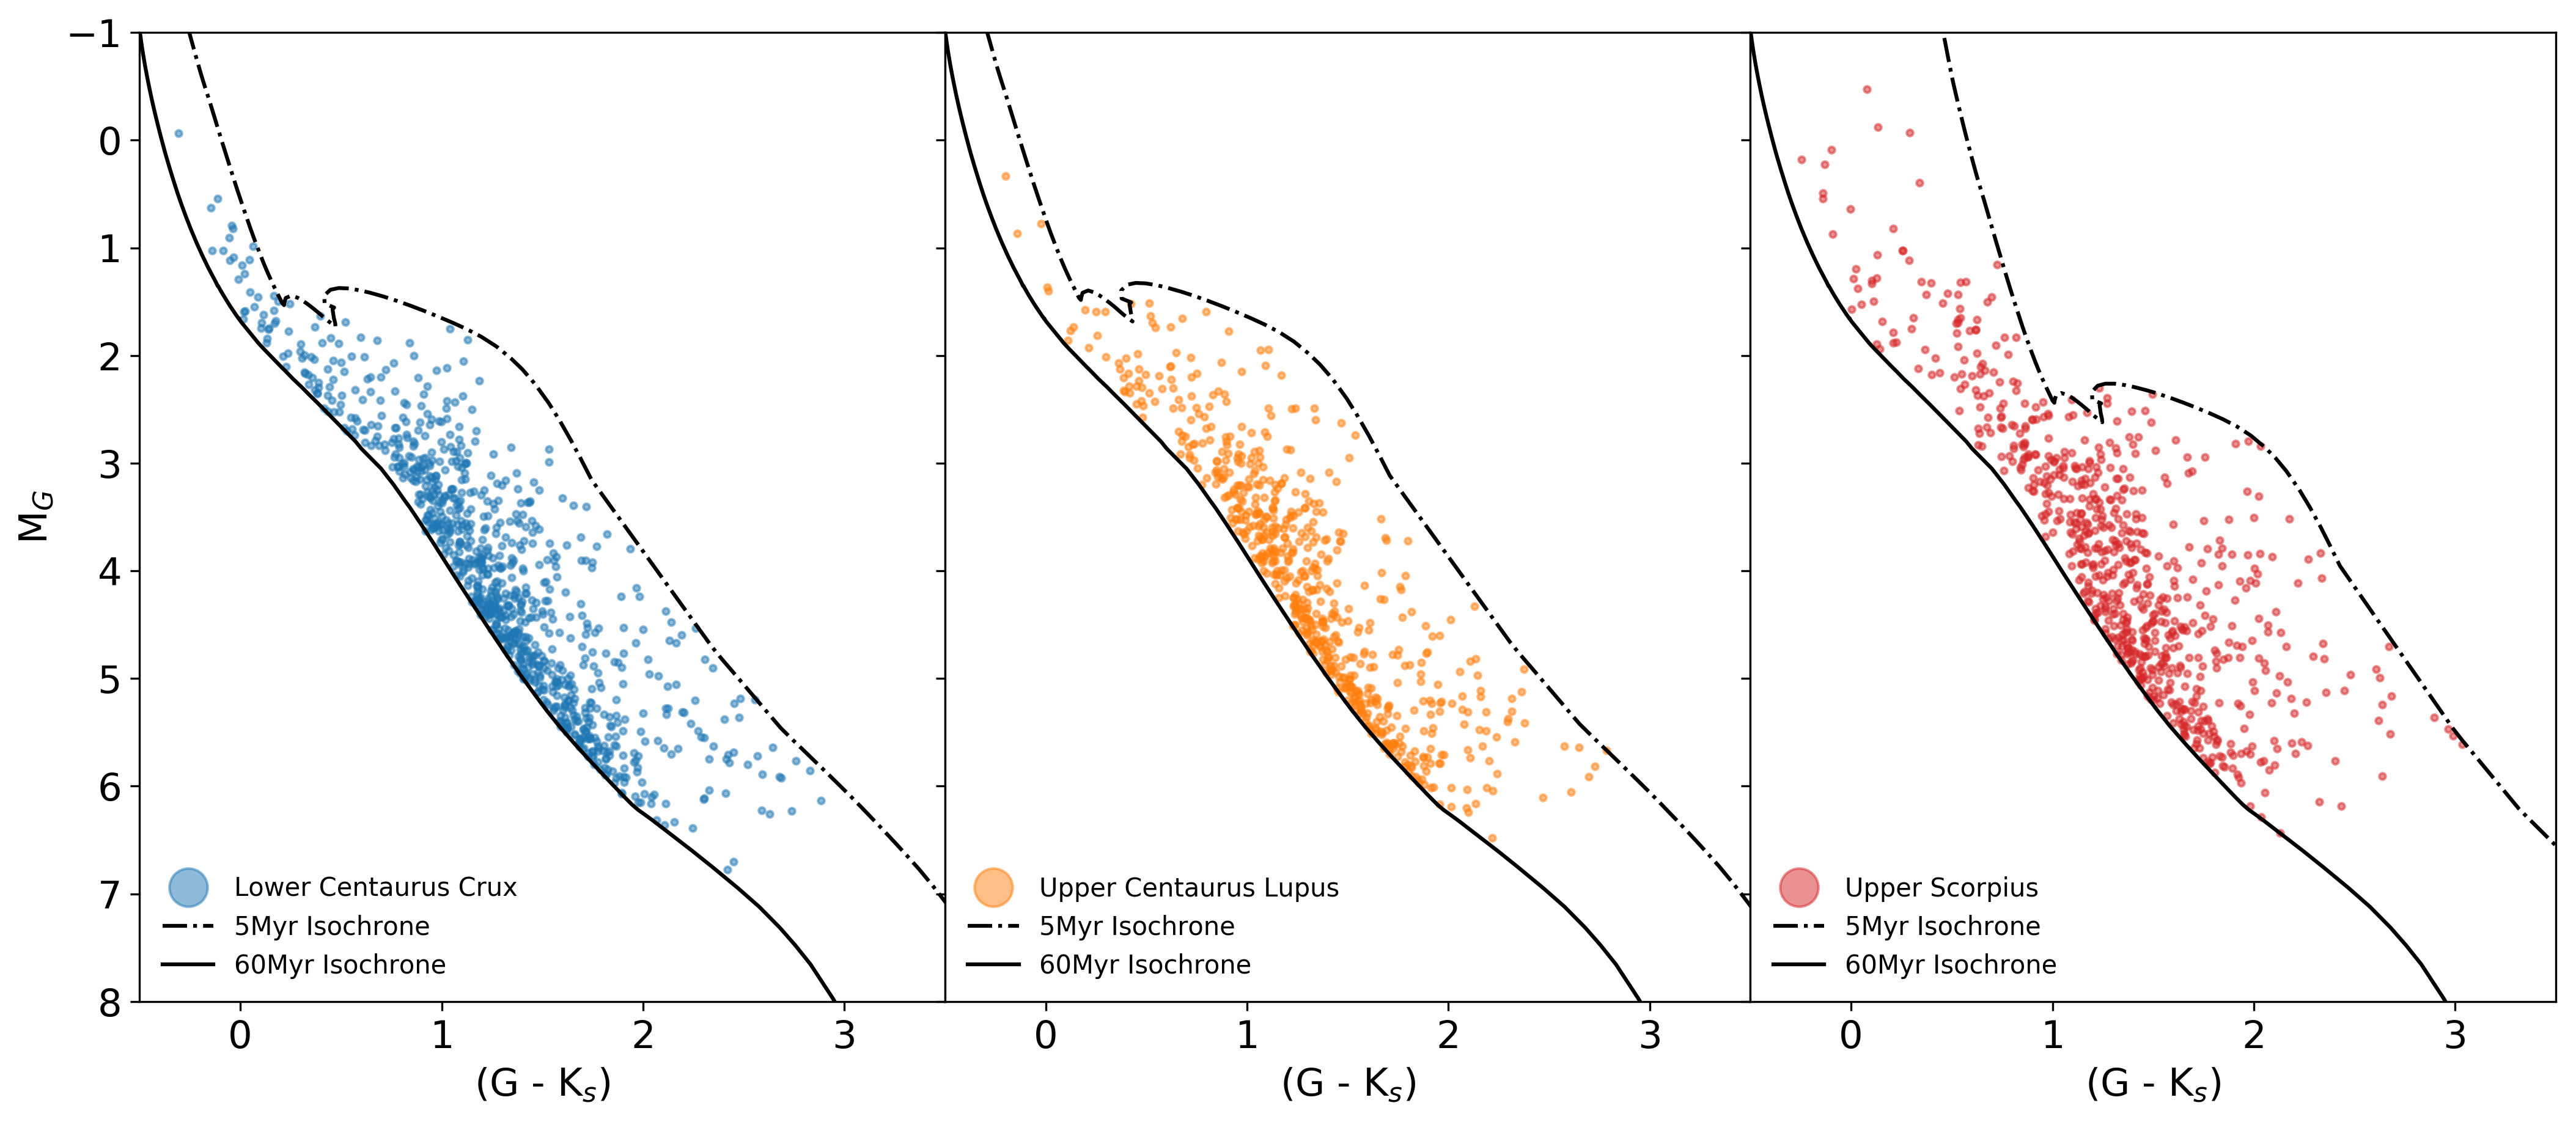
\includegraphics[width = 16cm, height = 8cm]{./Graficos/Capitulo_3/5_Sco-Cen/final_Sample_SCOCEN.png}} 
% \caption{\scriptsize{Color-magnitude diagrams for each subgroup in ScoCen using selected \textit{Gaia}-DR1 data between two different isochrones as in \autoref{fig:Isochrones_2}, along with isochrones using the extinction value measured proposed by \cauthor{1989A&A...216...44D} \citeyear{1989A&A...216...44D}. \textit{Left}: LCC stars after the dynamical and positional cuts are shown in blue. The black lines correspond to different isochrones. \textit{Center}: UCL stars after the dynamical and positional cuts are shown in orange. The black lines correspond to different isochrones. \textit{Right}: US stars after the dynamical and positional cuts are shown in red. The black lines correspond to different isochrones. Only the $5 \textnormal{Myr}$ to $60 \textnormal{Myr}$ isochrones were used to restrict the sample of stars to be inside this particular region. Following this, stars inside the region are quite likely to belong to the cluster and be in an stellar age range suitable for our study. In this case, the extinction values for LCC, UCL, and US correspond to $\textnormal{A}_\textnormal{v} = 0.23$, $\textnormal{A}_\textnormal{v} = 0.17$, and $\textnormal{A}_\textnormal{v} = 0.76$, respectively.}}
% \label{fig:Isochrones_4}
% \end{figure}

The main goal out of this process is to obtain a reliable sample which contains as much as possible stars which could be potential candidates to belong to the ScoCen association based on distance and dynamical properties derived from literature. As was stated before, this analysis was performed on a sample data using \textit{Gaia}-DR1, and the final sample is made of LCC $= 889$, UCL $= 644$, and US $= 705$ stars respectively, in which there is a slight increase in the number of stars per sub-region compared to the case in which no extinction is used as expected because the region between the isochrones is now larger.\\

In the next section, the same process described above to obtain the final sample but using the new data provided through \textit{Gaia}-DR2 is addressed. A few extra steps are needed due to new conditions imposed on parameters as color, parallax, and measurement errors which will be described in order to justify the selected stars which will be cross-matched to the \textit{SuperWASP} database.  

%============================================================================================================================================================

\section{\textit{Gaia}-DR2 Analysis}\label{sec:CleaningProcess}

Resolved or partially resolved binaries cause different kind of errors, for example when the different observations of a source variously refer to one or the other of the components, or to the photocentre, depending on the direction of the scan \cauthor{2018arXiv180409366L} (\citeyear{2018arXiv180409366L}). In some cases, this is known to produce spurious results, for instance, very large positive or negative parallaxes \cauthor{2017A&A...599A..50A} (\citeyear{2017A&A...599A..50A}). \textit{Gaia} DR2 contains a small number of sources with very large positive or negative parallaxes, for example exceeding $\pm 1$ arcsec. These are most likely produced by cross-matching issues, where different observation of the same nominal source is matched to different physical sources \cauthor{2018arXiv180409366L} (\citeyear{2018arXiv180409366L}). In such cases, the proper motion, in general, will also be corrupted. Thus, one must perform an extra clean process on the released data in order to correct for spurious sources and obtain a reliable scientific sample because no filtering was made in the \textit{Gaia} Archive based on the sizes of the parallaxes and proper motions. To perform this corrections and select astrometrically `clean' subsets we followed the method suggested in \textit{Appendix C} of \cauthor{2018arXiv180409366L} (\citeyear{2018arXiv180409366L}) and the main steps are described as follows.\\

The data provided in \textit{Gaia} DR2 satisfy a five-parameter solution which is accepted if the following conditions are met for the source:

\begin{enumerate}[label=(\roman*)]
\item mean magnitude $\textnormal{G} \leq 21.0$
\item \texttt{visibility\_periods\_used} $\geq 6$
\item \texttt{astrometric\_sigma5d\_max} $\leq~(1.2\textnormal{mas})\times\gamma(\textnormal{G})$
\end{enumerate}

where $\gamma(\textnormal{G}) = \textnormal{max}[1, 10^{0.2(G-18)}]$. This criterion was designed to include as many sources as possible with reasonably reliable astrometry \cauthor{2018arXiv180409366L} (\citeyear{2018arXiv180409366L}), though it must not be taken as fixed recipe for selecting sources with the most reliable astrometry, but it may provide useful hints for further exploration. Having said this, we proceeded to select our sample of stars given the parallax/proper motion (see \autoref{sec:GaiaSamples}) and coordinates (see \autoref{tab:ScoCen_SpatialDist}) limits for each one of the subgroups conforming ScoCen, and extra conditions on the parallax and photometry accuracy as given by, 

\begin{enumerate}[label=(\roman*)]
\item galactic coordinates as listed in \autoref{tab:ScoCen_SpatialDist} and parallaxes given in \cauthor{2016MNRAS.461..794P} (\citeyear{2016MNRAS.461..794P})
\item $\varpi/\sigma_\varpi > 10$
\item \texttt{phot\_bp\_mean\_flux\_over\_error} $> 10$
\item \texttt{phot\_rp\_mean\_flux\_over\_error} $> 10$
\end{enumerate}

Nominally, \textit{(i)} selects sources satisfying the galactic coordinates, and parallax and proper motion cuts, \textit{(ii)} those with at most $10\%$ uncertainty in distance (corresponding to $\simeq 0.2 \textnormal{mag}$ in absolute magnitude), and \textit{(iii)}-\textit{(iv)} those with at most $10\%$ uncertainty in the BP and RP fluxes (corresponding to $\simeq 0.1 \textnormal{mag}$ in $\textnormal{G}_\textnormal{BP}$ and $\textnormal{G}_\textnormal{RP}$). Taken at face value, this selection should produce a quite cleaned HR-diagram. However it is reasonable to expect that in most such cases of spurious parallaxes, observations do not fit the single-stellar parallax model very well leading to an increase in the $\chi^2$ affecting the unit weight error, defined as $u = (\chi^2/\nu)^{1/2}$ in \cauthor{2018arXiv180409366L} (\citeyear{2018arXiv180409366L}). The $\chi^2$ is obtained from the \textit{Gaia} Archive and is given as a column named \texttt{astrometric\_chi2\_al}, and $\nu$ represents the degrees of freedom which can be computed as \texttt{astrometric\_n\_good\_obs\_al}$-5$, accounting for the acceptance model described above.\\

In \autoref{fig:LindegrenSelection}, the unit weight error (e.g. $\textnormal{u}^2$; \autoref{eq:WeightError}) is shown as a function of the absolute magnitude in band-G for each one of the three subgroups in ScoCen. \cauthor{2018arXiv180409366L} (\citeyear{2018arXiv180409366L}) considered all the possible stars within $100~\textnormal{pc}$ and realized that a strong rise in $\textnormal{G} < 6$ is caused by uncalibrated CCD saturation; also a blob of moderately large values of $\textnormal{u}$ for $\textnormal{G} > 18$ possibly extending to larger values for brighter sources; and a general scatter of large $\textnormal{u}$ at all magnitudes, possibly caused by partially resolved or astrometric binaries. Thus, if sources with $\textnormal{G} < 6$ which basically includes most of the giants are to be kept while removing the blob at $\textnormal{G} > 18$ the possible cut is given by the square root of \autoref{eq:WeightError}, however, as we have a different sample, we decided to clean without considering the square root. Besides, additional scatter in the Hertzsprung-Russell diagram is produced by photometric errors mainly in the $\textnormal{G}_\textnormal{BP}$ and $\textnormal{G}_\textnormal{RP}$ bands, affecting crowded areas, in particular with faint sources. An indicator of possible issues with the $\textnormal{G}_\textnormal{BP}$ and $\textnormal{G}_\textnormal{RP}$ photometry is given in the \textit{Gaia} DR2 as the flux error factor $\textnormal{E} = (\textnormal{I}_\textnormal{BP} + \textnormal{I}_\textnormal{RP}) / \textnormal{I}_\textnormal{G}$ (\texttt{phot\_bp\_rp\_excess\_factor}), where each $\textnormal{I}_\textnormal{x}$ corresponds to the flux in band $\textnormal{x}$ as shown in \cauthor{2017A&A...600A..51E} (\citeyear{2017A&A...600A..51E}). Following \cauthor{2018arXiv180409366L} (\citeyear{2018arXiv180409366L}), the flux excess can be restricted using $1.0 + 0.015(\textnormal{G}_\textnormal{BP}-\textnormal{G}_\textnormal{RP})^2 < \textnormal{E} < 1.3 + 0.06(\textnormal{G}_\textnormal{BP}-\textnormal{G}_\textnormal{RP})^2$. After all this cleaning process is applied, some scatter still can be present between the main and white-dwarf sequences (see \autoref{fig:FinalSample_DR2}) which could be partly real, consisting of binaries with white-dwarf and main-sequence companions of roughly equal magnitude. Roughly equal number of of positive and negative spurious parallaxes can be present due to different observations of the same \textit{Gaia} source being matched to two (or more) physically distinct objects.

\begingroup
\large
\begin{equation}
  \textnormal{u}^2 = \frac{\chi^2}{\nu} < 1.4 \times \textnormal{max} (~1, \textnormal{exp(~-0.4(~\textnormal{G} - 19.5~)~)}~)
 \label{eq:WeightError}
\end{equation}
\endgroup \\

% \begin{figure}[!ht]
% \centering
%   \subfloat{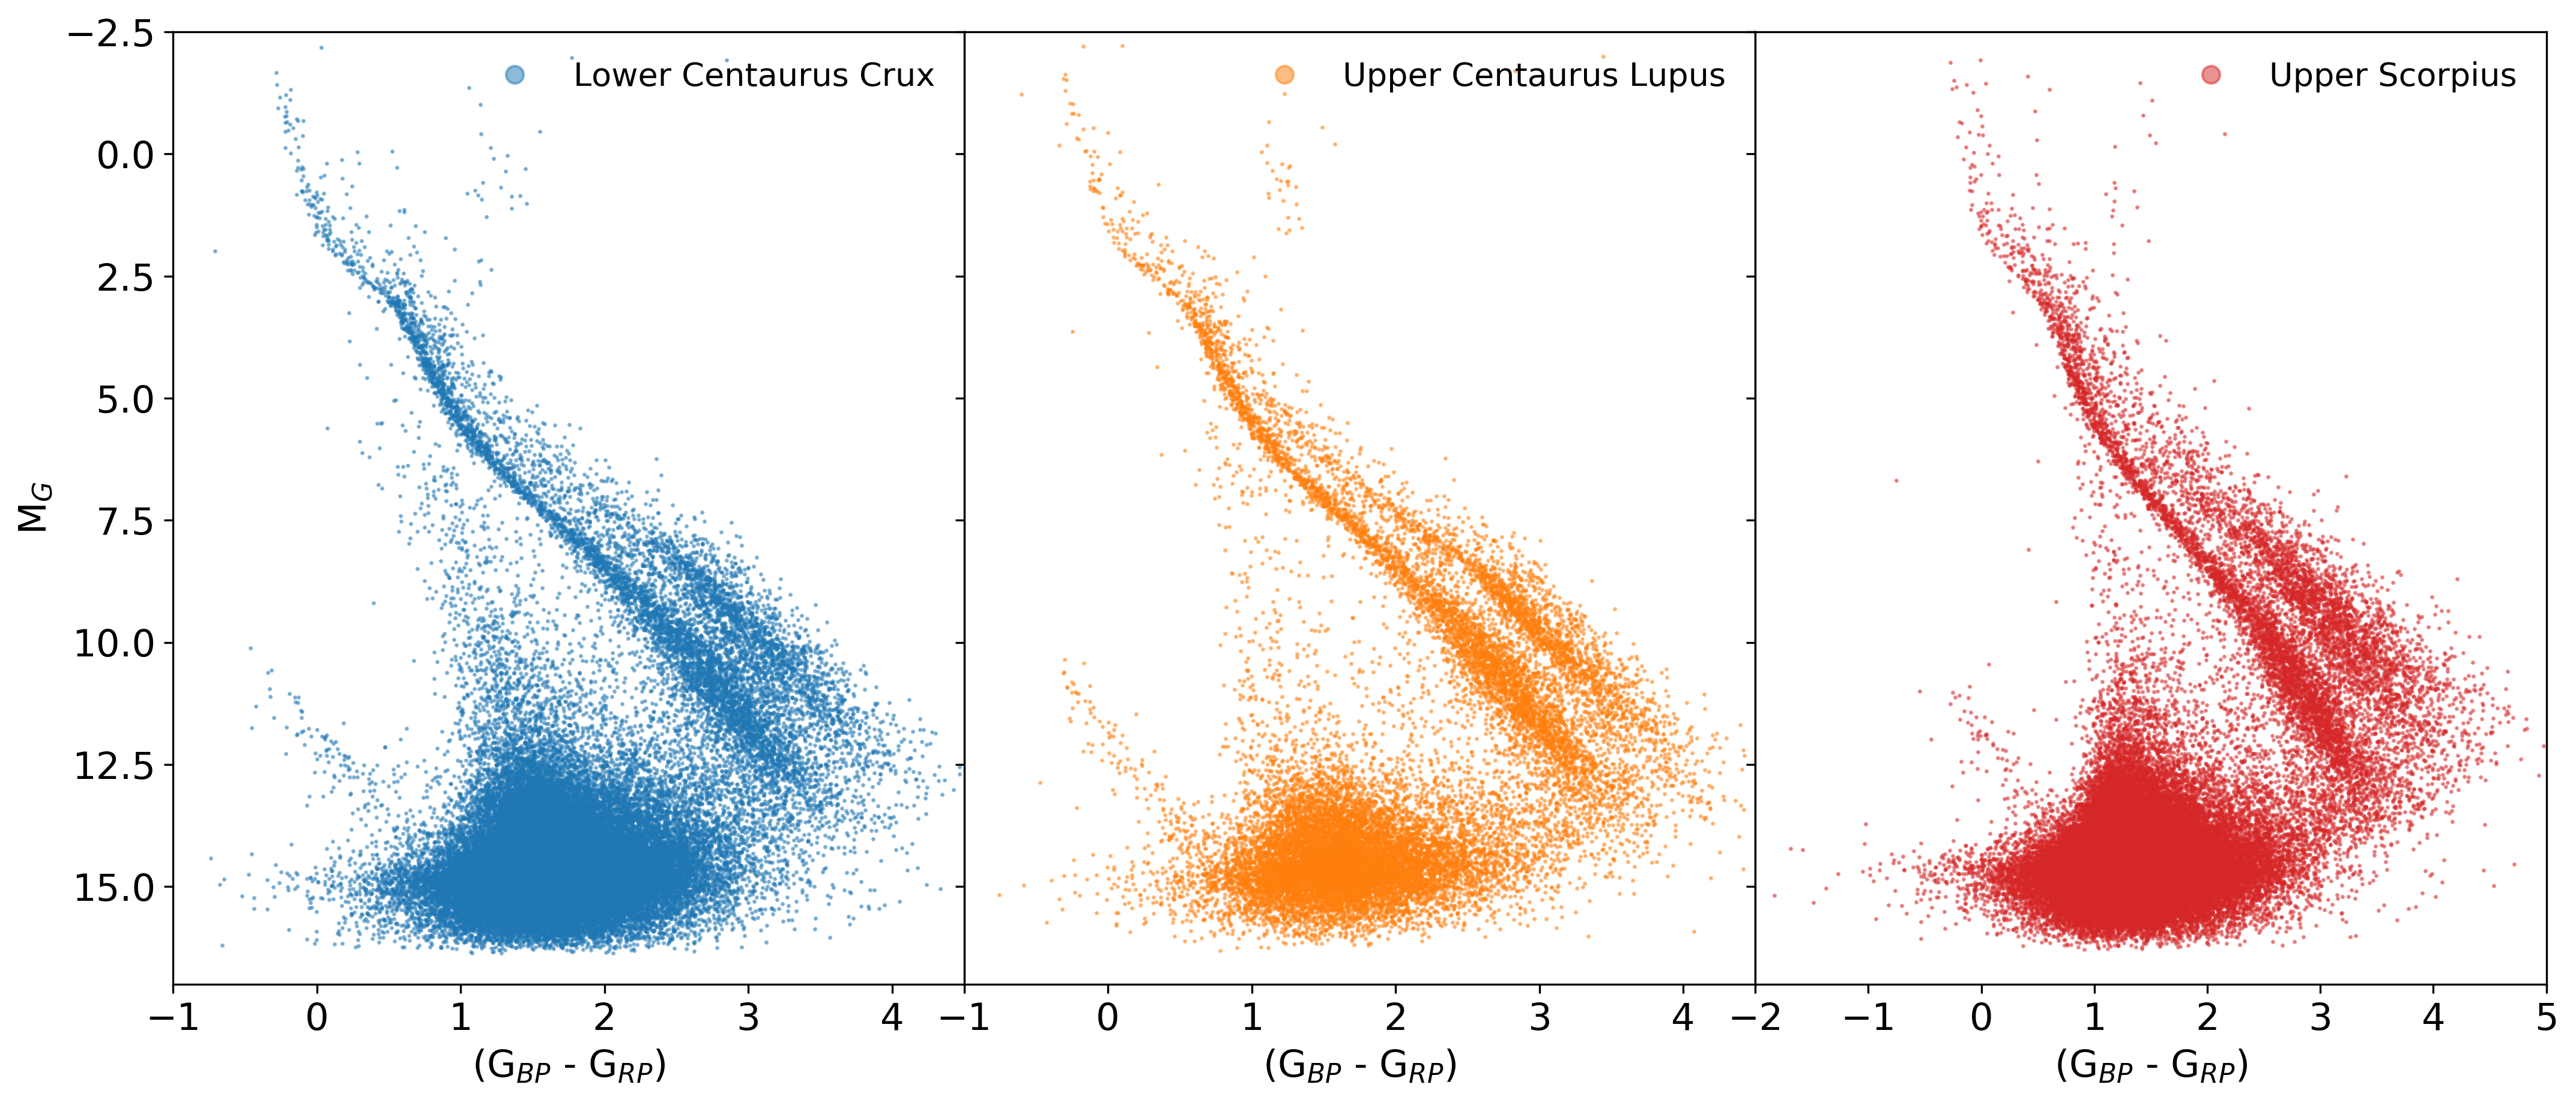
\includegraphics[width = 16cm, height = 7.5cm]{./Graficos/Capitulo_3/7_DR2_LightCurves/DR2_Sample_NoSelection_2_2.png}} 
% \caption{\scriptsize{Color-magnitude diagram using \textit{Gaia}-DR2 data for each subgroup in ScoCen. \textit{Left}: LCC absolute magnitude in the $\textnormal{G}$-band as a function of color-index $\textnormal{G}_\textnormal{BP} - \textnormal{G}_\textnormal{RP}$. \textit{Center}: UCL absolute magnitude in the $\textnormal{G}$-band as a function of color-index $\textnormal{G}_\textnormal{BP} - \textnormal{G}_\textnormal{RP}$. \textit{Right}: US absolute magnitude in the $\textnormal{G}$-band as a function of color-index $\textnormal{G}_\textnormal{BP} - \textnormal{G}_\textnormal{RP}$. In contrast to \textit{Gaia}-DR1, the new data sample contains more stars in each subgroup, and stars with absolute magnitude up to $\textnormal{M}_\textnormal{G} > 17$.}}
% \label{fig:NewData_DR2}
% \end{figure}
% 
% \begin{figure}[!ht]
% \centering
%   \subfloat{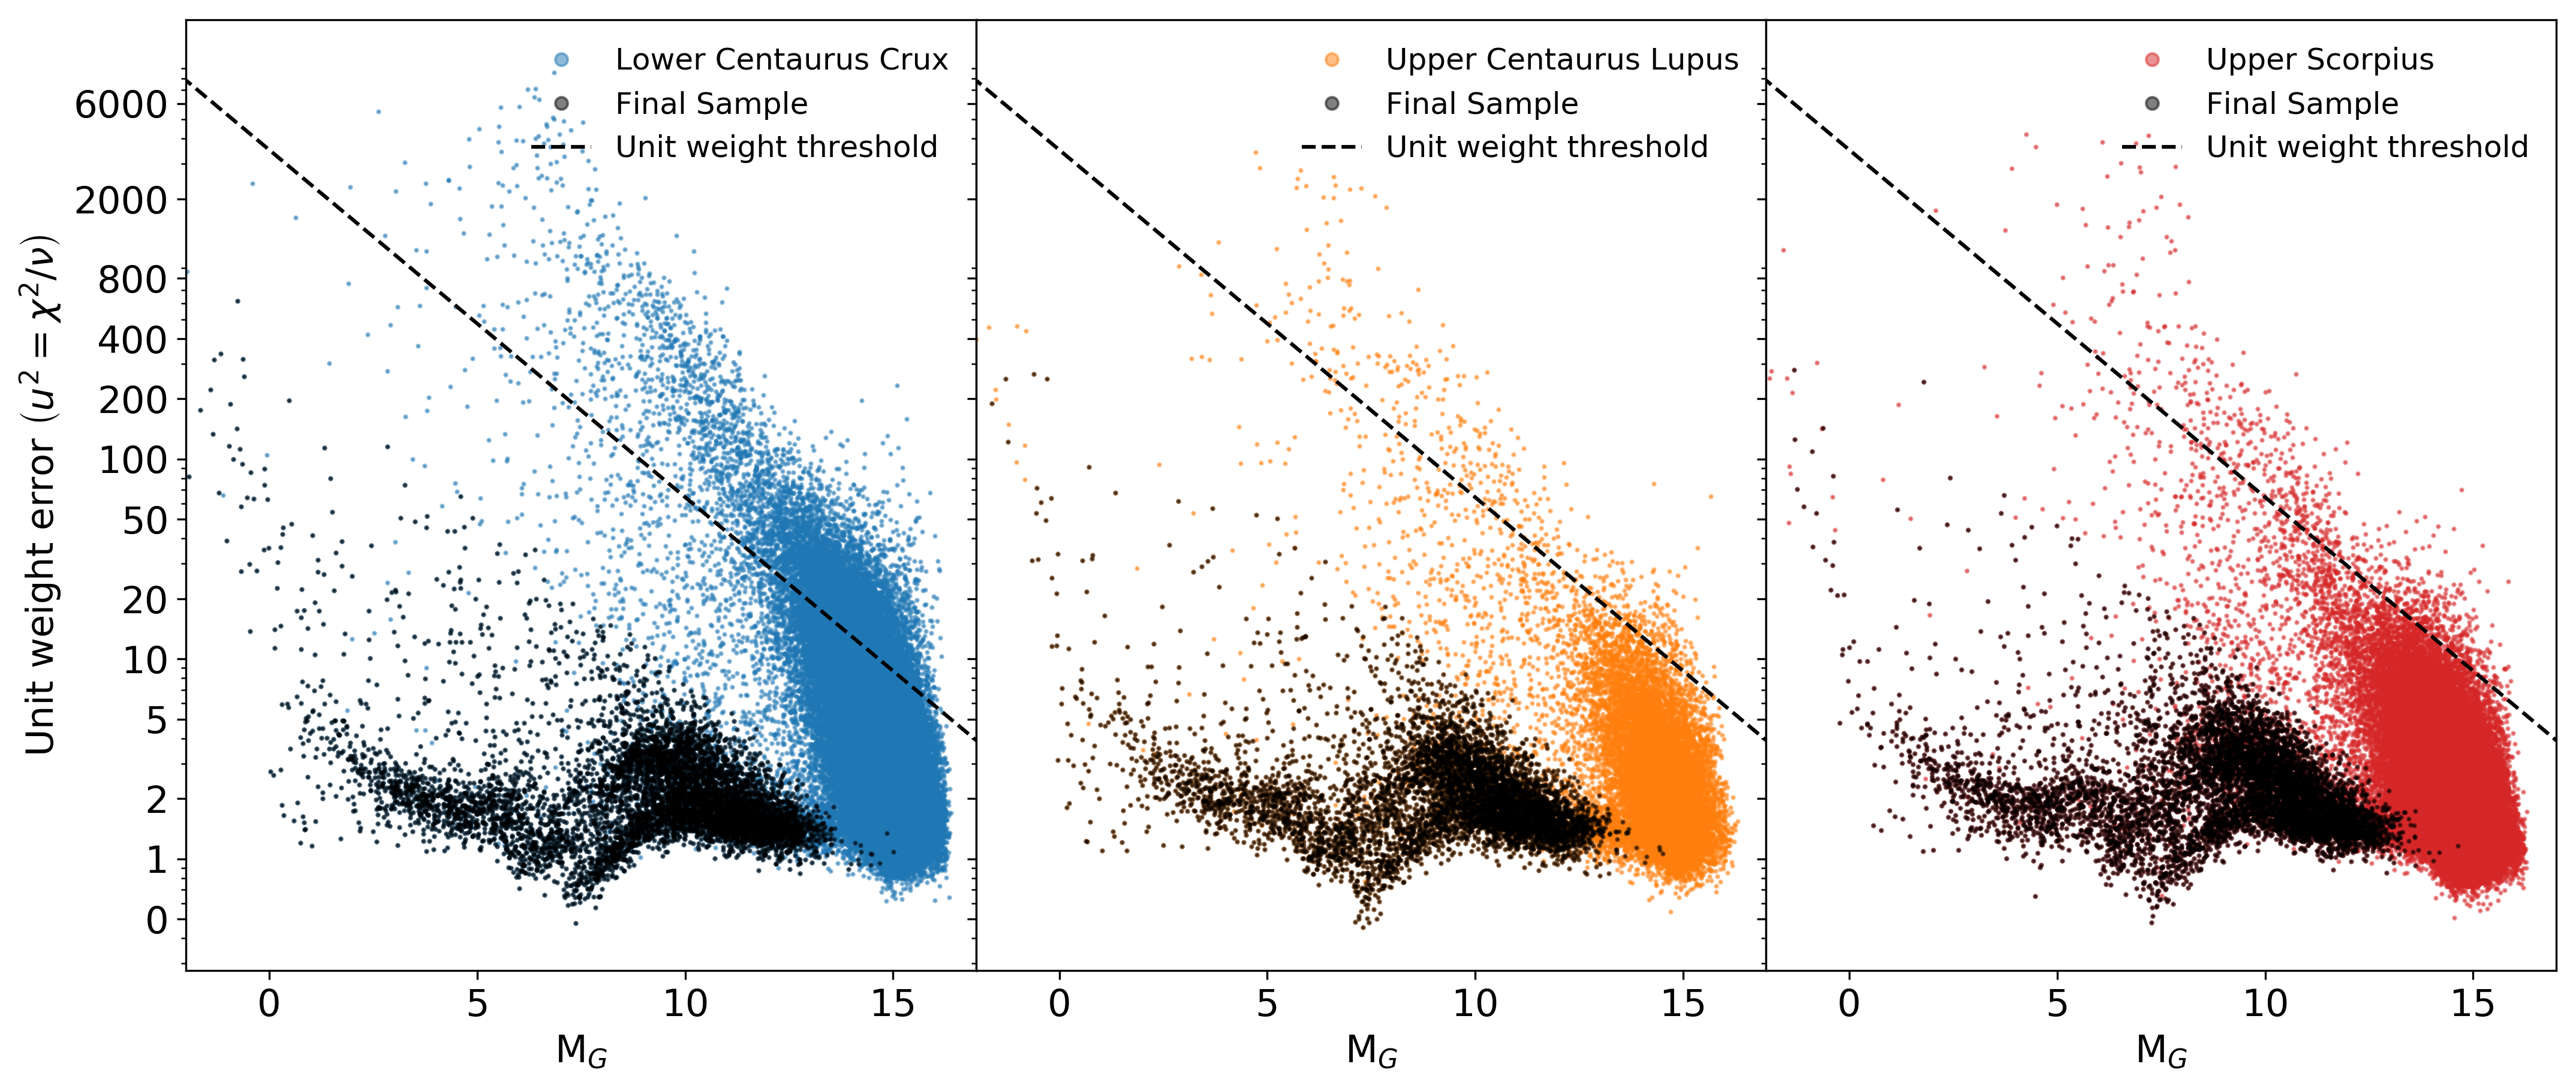
\includegraphics[width = 16cm, height = 7.5cm]{./Graficos/Capitulo_3/7_DR2_LightCurves/Lindegren_Selection.png}} 
% \caption{\scriptsize{Unit weight error threshold as proposed by \cauthor{2016ApJS..222....8D} \citeyear{2016ApJS..222....8D} to obtain photometric and astrometric cleaned data. The black line represents the threshold defined in \autoref{eq:WeightError}. \textit{Left}: LCC unit weight error as a function of magnitude in the $\textnormal{G}$-band. The blue dots represents the original sample as shown in \autoref{fig:NewData_DR2}-left panel, while the black dots correspond to the filtered by unit weight error and flux excess ratio. \textit{Center}: UCL unit weight error as a function of magnitude in the $\textnormal{G}$-band. The orange dots represents the original sample as shown in \autoref{fig:NewData_DR2}-center panel, while the black dots correspond to the filtered by unit weight error and flux excess ratio. \textit{Right}: US unit weight error as a function of magnitude in the $\textnormal{G}$-band. The red dots represents the original sample as shown in \autoref{fig:NewData_DR2}-right panel, while the black dots correspond to the filtered by unit weight error and flux excess ratio.}}
% \label{fig:LindegrenSelection}
% \end{figure}
% 
% \begin{figure}[!ht]
% \centering
%   \subfloat{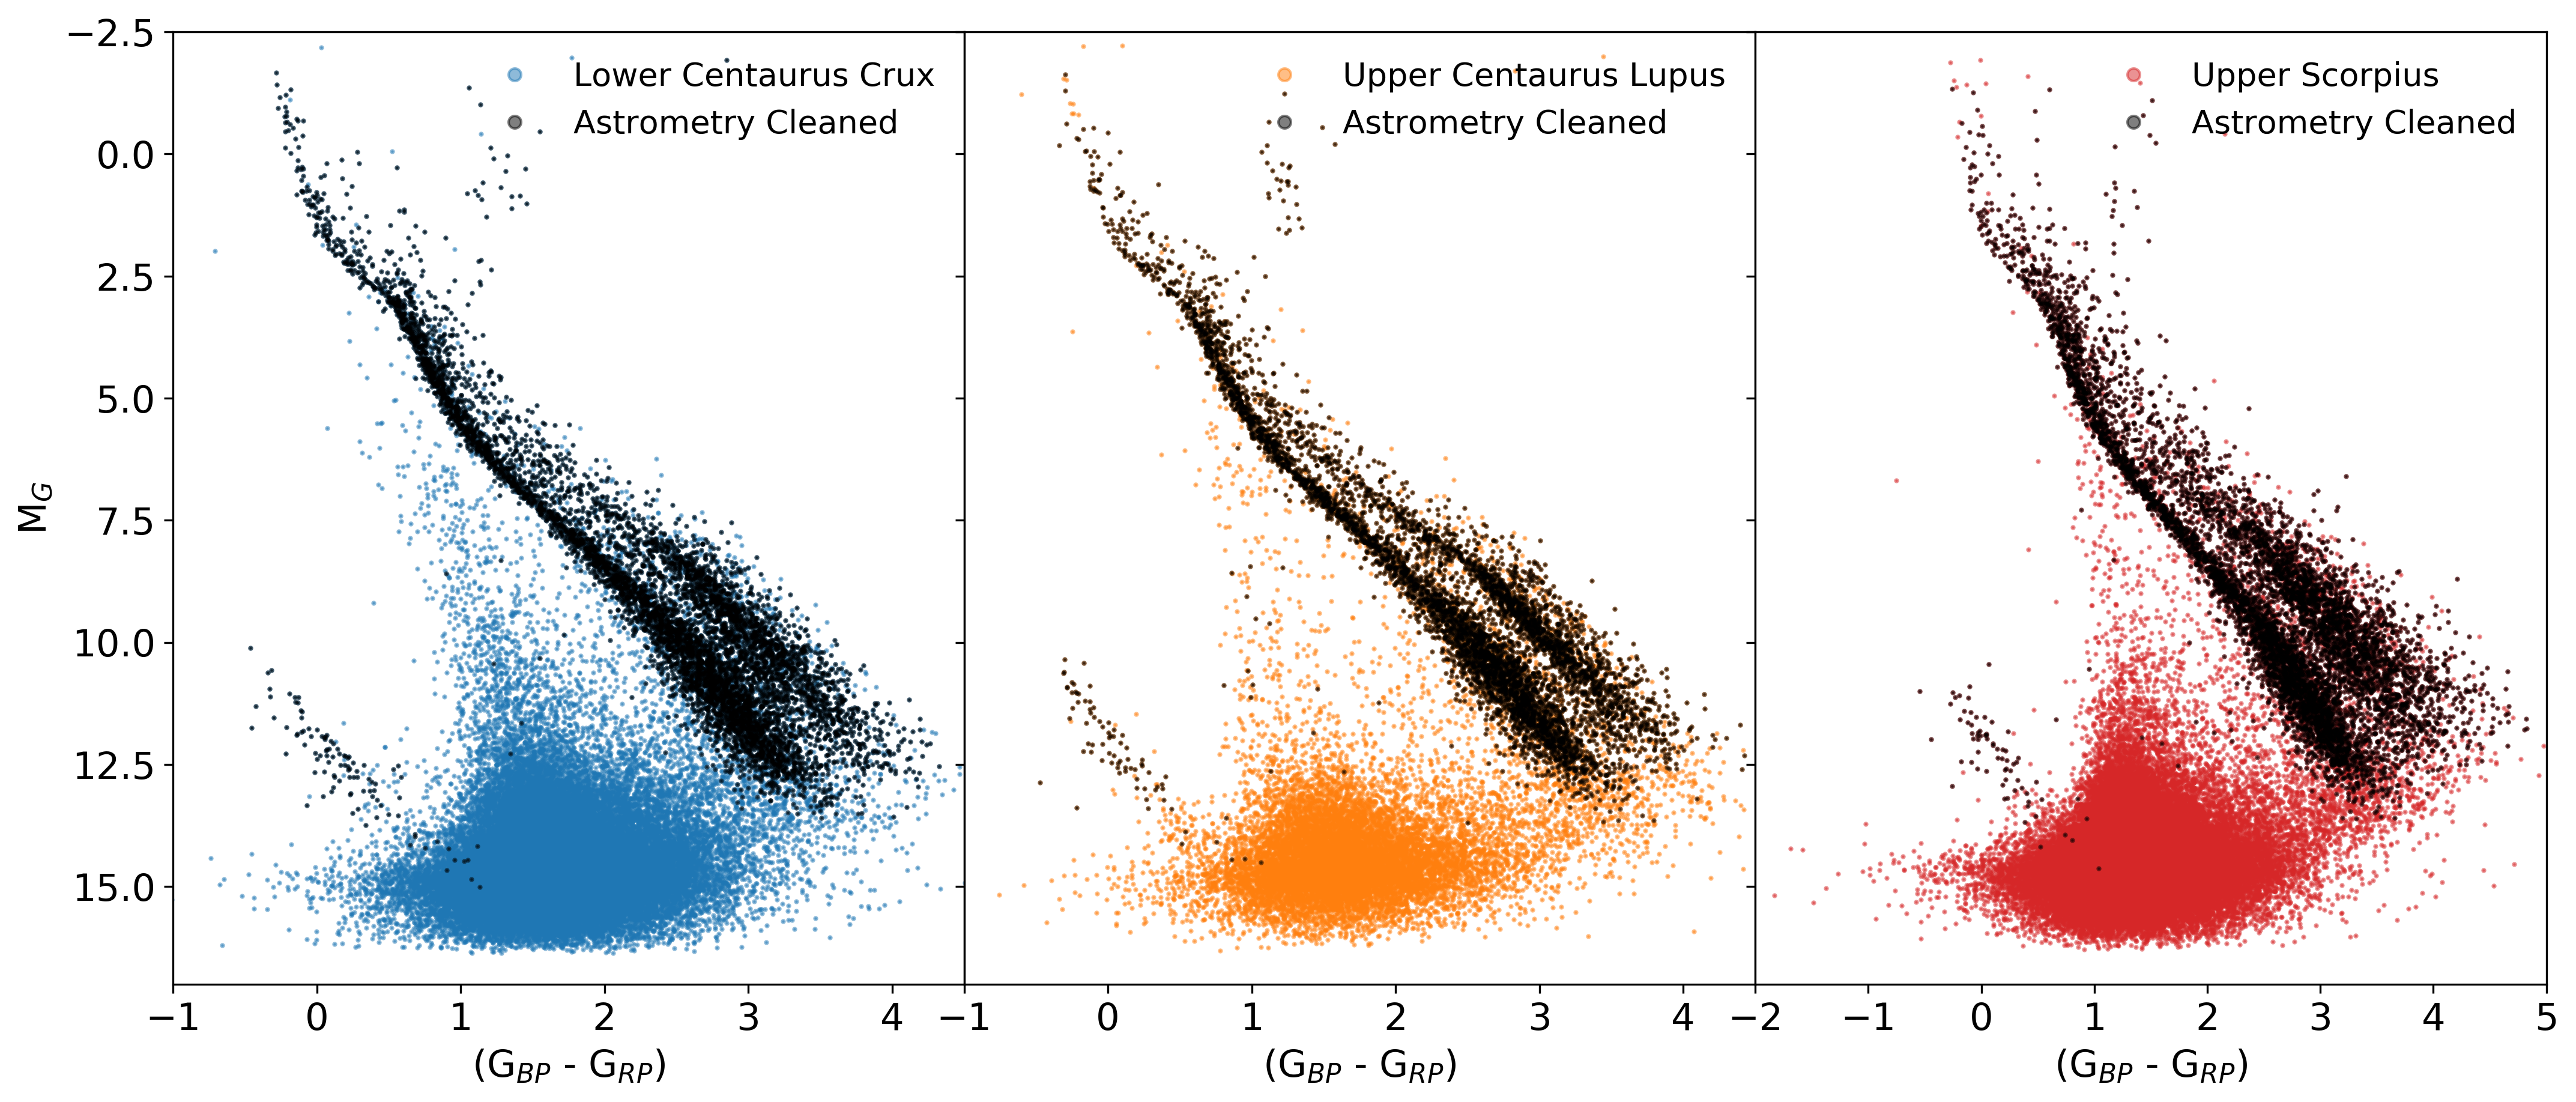
\includegraphics[width = 15.5cm, height = 7.5cm]{./Graficos/Capitulo_3/7_DR2_LightCurves/CMD_Cleaned_MG.png}} 
% \caption{\scriptsize{Color-magnitude diagram using \textit{Gaia}-DR2 data for each subgroup in ScoCen filtered by unit weight error and flux excess ratio. \textit{Left}: LCC absolute magnitude in the $\textnormal{G}$-band as a function of color-index $\textnormal{G}_\textnormal{BP} - \textnormal{G}_\textnormal{RP}$. \textit{Center}: UCL absolute magnitude in the $\textnormal{G}$-band as a function of color-index $\textnormal{G}_\textnormal{BP} - \textnormal{G}_\textnormal{RP}$. \textit{Right}: US absolute magnitude in the $\textnormal{G}$-band as a function of color-index $\textnormal{G}_\textnormal{BP} - \textnormal{G}_\textnormal{RP}$. The color dots show the original sample as presented in \autoref{fig:NewData_DR2}, while the black dots correspond to the final sample after correcting the flux excess ratio and unit weight error as shown in \autoref{fig:LindegrenSelection}.}}
% \label{fig:FinalSample_DR2}
% \end{figure}

In the original data retrieved using \textit{Gaia} DR2 we obtained $15\,074$, $9\,658$, and $14\,580$ for LCC, UCL, and US respectively. After performing the cleaning process to correct for spurious parallaxes and colors, we end up with a sample of $7\,268$, $6\,244$, and $7\,436$ for LCC, UCL, and US respectively (see \autoref{fig:LindegrenSelection}). In comparison to \textit{Gaia} DR1 an increase in sources is noticeable, specially for $\textnormal{M}_\textnormal{G} > 7$ (see \autoref{fig:Isochrones_4}). Also, there is a clear division between the pre-main sequence and the main-sequence population in each one of the subgroups, exposing how powerful \textit{Gaia} DR2 can be. Exactly the same selection process applied to the \textit{Gaia} DR1 was done to this new sample in order to select the stars and lately cross-match them with the \textit{SuperWASP} database and obtain the light curves. In \autoref{fig:DR2_Comparison}, the absolute magnitude in band-G as a function of color is presented for each subgroup. The two lines correspond to $5$Myr and $60$Myr isochrones, where the youngest isochrone has been computed using the mean extinction values calculated in \autoref{fig:SCOCEN_Extinction}. The final sample corresponds to stars between both isochrones. As can be observed in \autoref{fig:DR2_Comparison} and \autoref{fig:DR2_Selection}, the isochrones models have a lower limit in absolute magnitude around $\textnormal{M}_\textnormal{G} \backsimeq 10$, at least for the $5$Myr isochrone. Thus, we decided to cut in this values, although an interpolation of the isochrones is possible if one wants to go down to lower values in absolute magnitude which means obtaining more low-mass stars. This is clearly seen in \autoref{fig:DR2_Tracks} where different stellar tracks are shown for selected stars to check how low in stellar mass we can go with the new data set. Using \textit{Gaia} DR1 we had a limit close to $\sim0.9\textnormal{M}_\odot$ (see \autoref{fig:Stellar_Tracks_3}) however, with \textit{Gaia} DR2   this limit has gone down to $\sim0.1\textnormal{M}_\odot$ which is indeed the limit of the stellar track models. It is worthy to note that if we do not perform any cut in absolute magnitude, we can go down to $\textnormal{M}_\textnormal{G}\sim14$, which basically means that if we compare \autoref{fig:DR2_Comparison} and \autoref{fig:DR2_Selection} we can include a huge sample of quite low-mass stars which are out of our final sample. This could be addressed in a future work to compare how much the pre-selection in \textit{Gaia} DR2 and the cross-matching with the \textit{SuperWASP} changes. Having said that, we can guarantee that the final sample has enough low-mass stars in the ScoCen OB association to be studied in more detail as these are the type of stars likely to show exoplanetary ring transits. Additionally, to verify that the final sample corresponds to the original sky selection after all the cleaning- and -selection process, the sky distribution is shown in \autoref{fig:DR2_Projection} for each one of the subgroups in a Hammer-Aitoff projection using Galactic coordinates.     

\begin{figure}[!ht]
\centering
  \subfloat{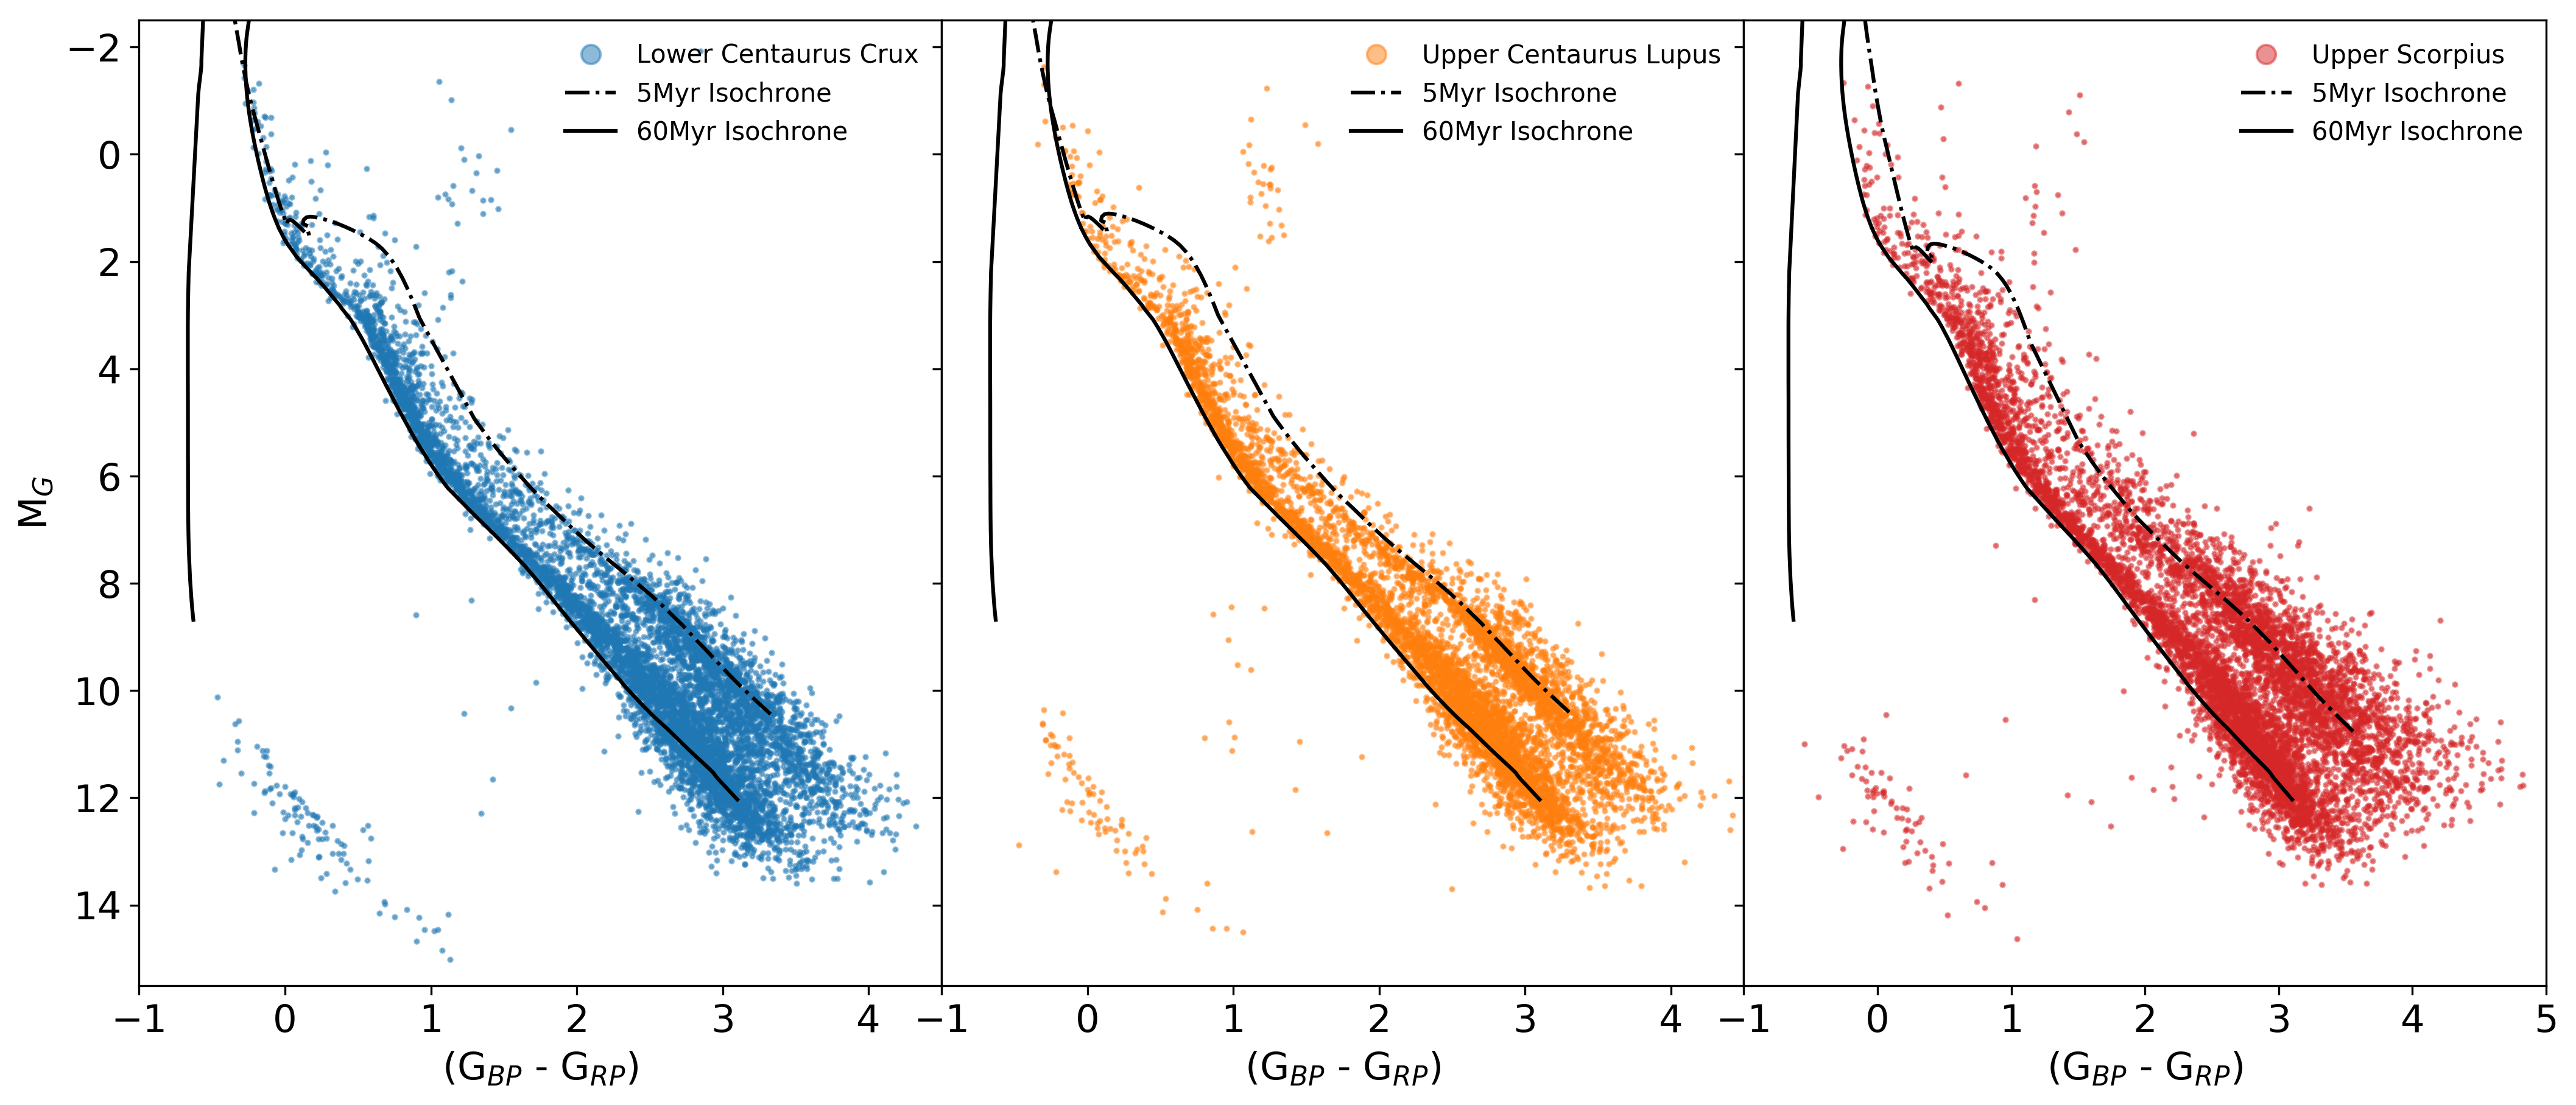
\includegraphics[width = 16cm, height = 7.5cm]{./Graficos/Capitulo_3/7_DR2_LightCurves/CMD_Clean_Iscohrones.png}} 
\caption{\scriptsize{Color-magnitude diagram using the filtered out sample for each subgroup in ScoCen as presented in \autoref{fig:FinalSample_DR2}. \textit{\textbf{Left}}: LCC absolute magnitude in the $\textnormal{G}$-band as a function of color-index $\textnormal{G}_\textnormal{BP} - \textnormal{G}_\textnormal{RP}$. \textit{\textbf{Center}}: UCL absolute magnitude in the $\textnormal{G}$-band as a function of color-index $\textnormal{G}_\textnormal{BP} - \textnormal{G}_\textnormal{RP}$. \textit{\textbf{Right}}: US absolute magnitude in the $\textnormal{G}$-band as a function of color-index $\textnormal{G}_\textnormal{BP} - \textnormal{G}_\textnormal{RP}$. The color dots represent the cleaned data, while the lines show two isochrones of $5 \textnormal{Myr}$, and $60 \textnormal{Myr}$, respectively, computed using $\textnormal{A}_\textnormal{v} = 0.23$, $\textnormal{A}_\textnormal{v} = 0.17$, and $\textnormal{A}_\textnormal{v} = 0.76$, for each subgroup. The new isochrones are computed with updated bandpasses corresponding to the \textit{Gaia}-DR2 using \textit{MIST}-package.}}
\label{fig:DR2_Comparison}
\end{figure}

\begin{figure}[!ht]
\centering
  \subfloat{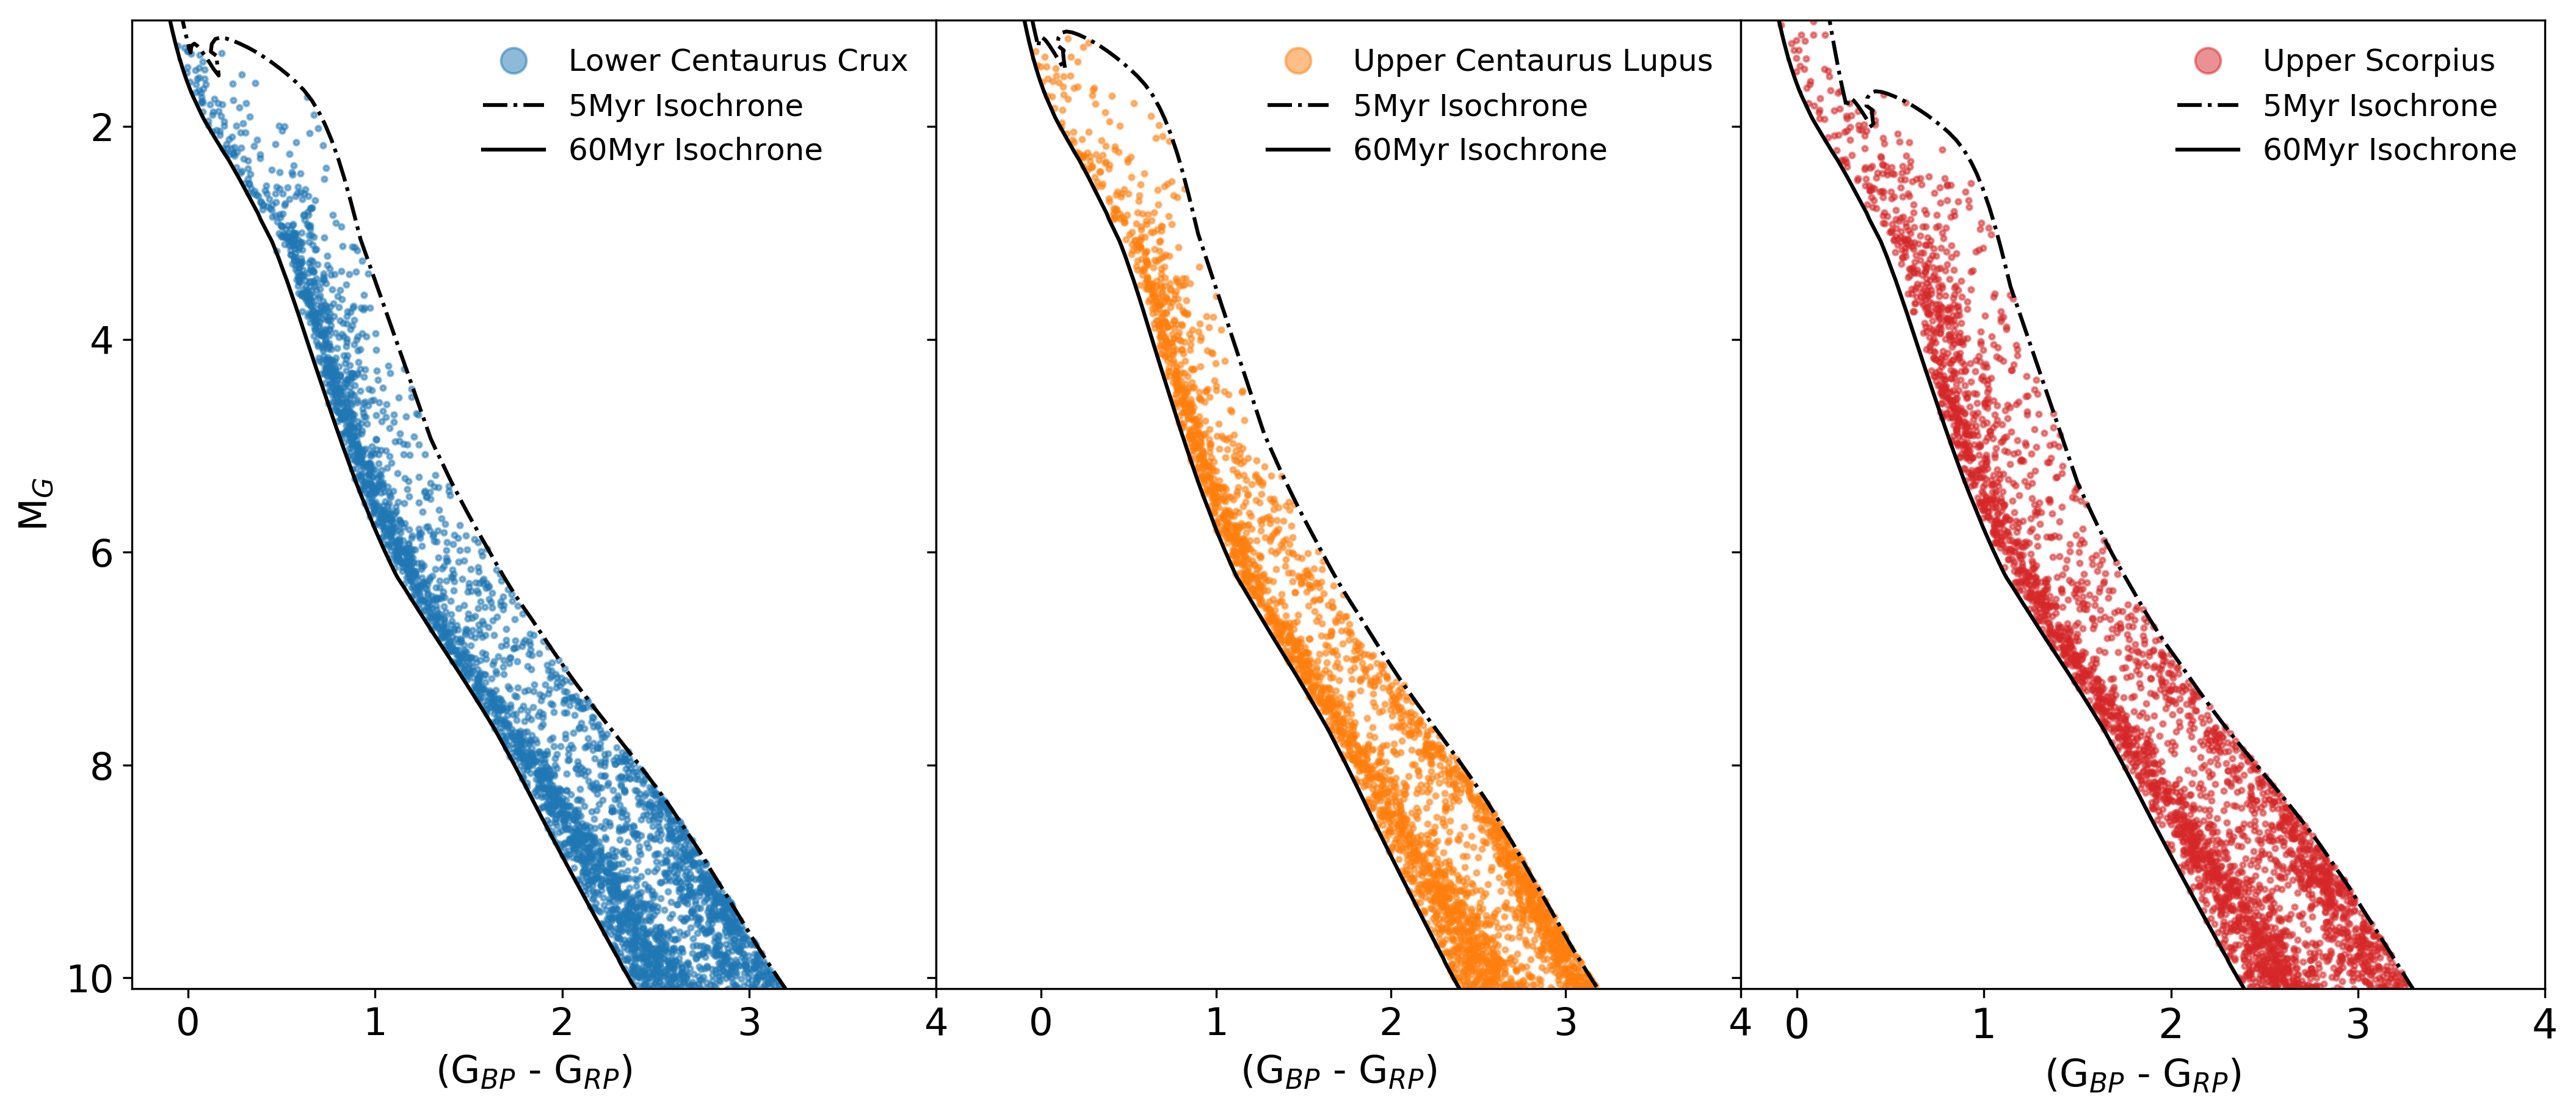
\includegraphics[width = 16cm, height = 7.5cm]{./Graficos/Capitulo_3/7_DR2_LightCurves/CMD_Clean_FinalSelection.png}} 
\caption{\scriptsize{Color-magnitude diagrams for each subgroup in ScoCen using the filtered out sample between two different isochrones applying the extinction value proposed by \cauthor{1989A&A...216...44D} (\citeyear{1989A&A...216...44D}). \textit{\textbf{Left}}: LCC stars after cuts are shown in blue. The black lines correspond to different isochrones. \textit{\textbf{Center}}: UCL stars after cuts are shown in orange. The black lines correspond to different isochrones. \textit{\textbf{Right}}: US stars after cuts are shown in red. The black lines correspond to different isochrones. Only the $5 \textnormal{Myr}$ to $60 \textnormal{Myr}$ isochrones were used to restrict the sample of stars to be inside this particular region. Following this, stars inside the region are quite likely to belong to the cluster and be in an stellar age range suitable for our study. In this case, the extinction values for LCC, UCL, and US correspond to $\textnormal{A}_\textnormal{v} = 0.23$, $\textnormal{A}_\textnormal{v} = 0.17$, and $\textnormal{A}_\textnormal{v} = 0.76$, respectively.}}
\label{fig:DR2_Selection}
\end{figure}

\begin{figure}[!ht]
\centering
  \subfloat{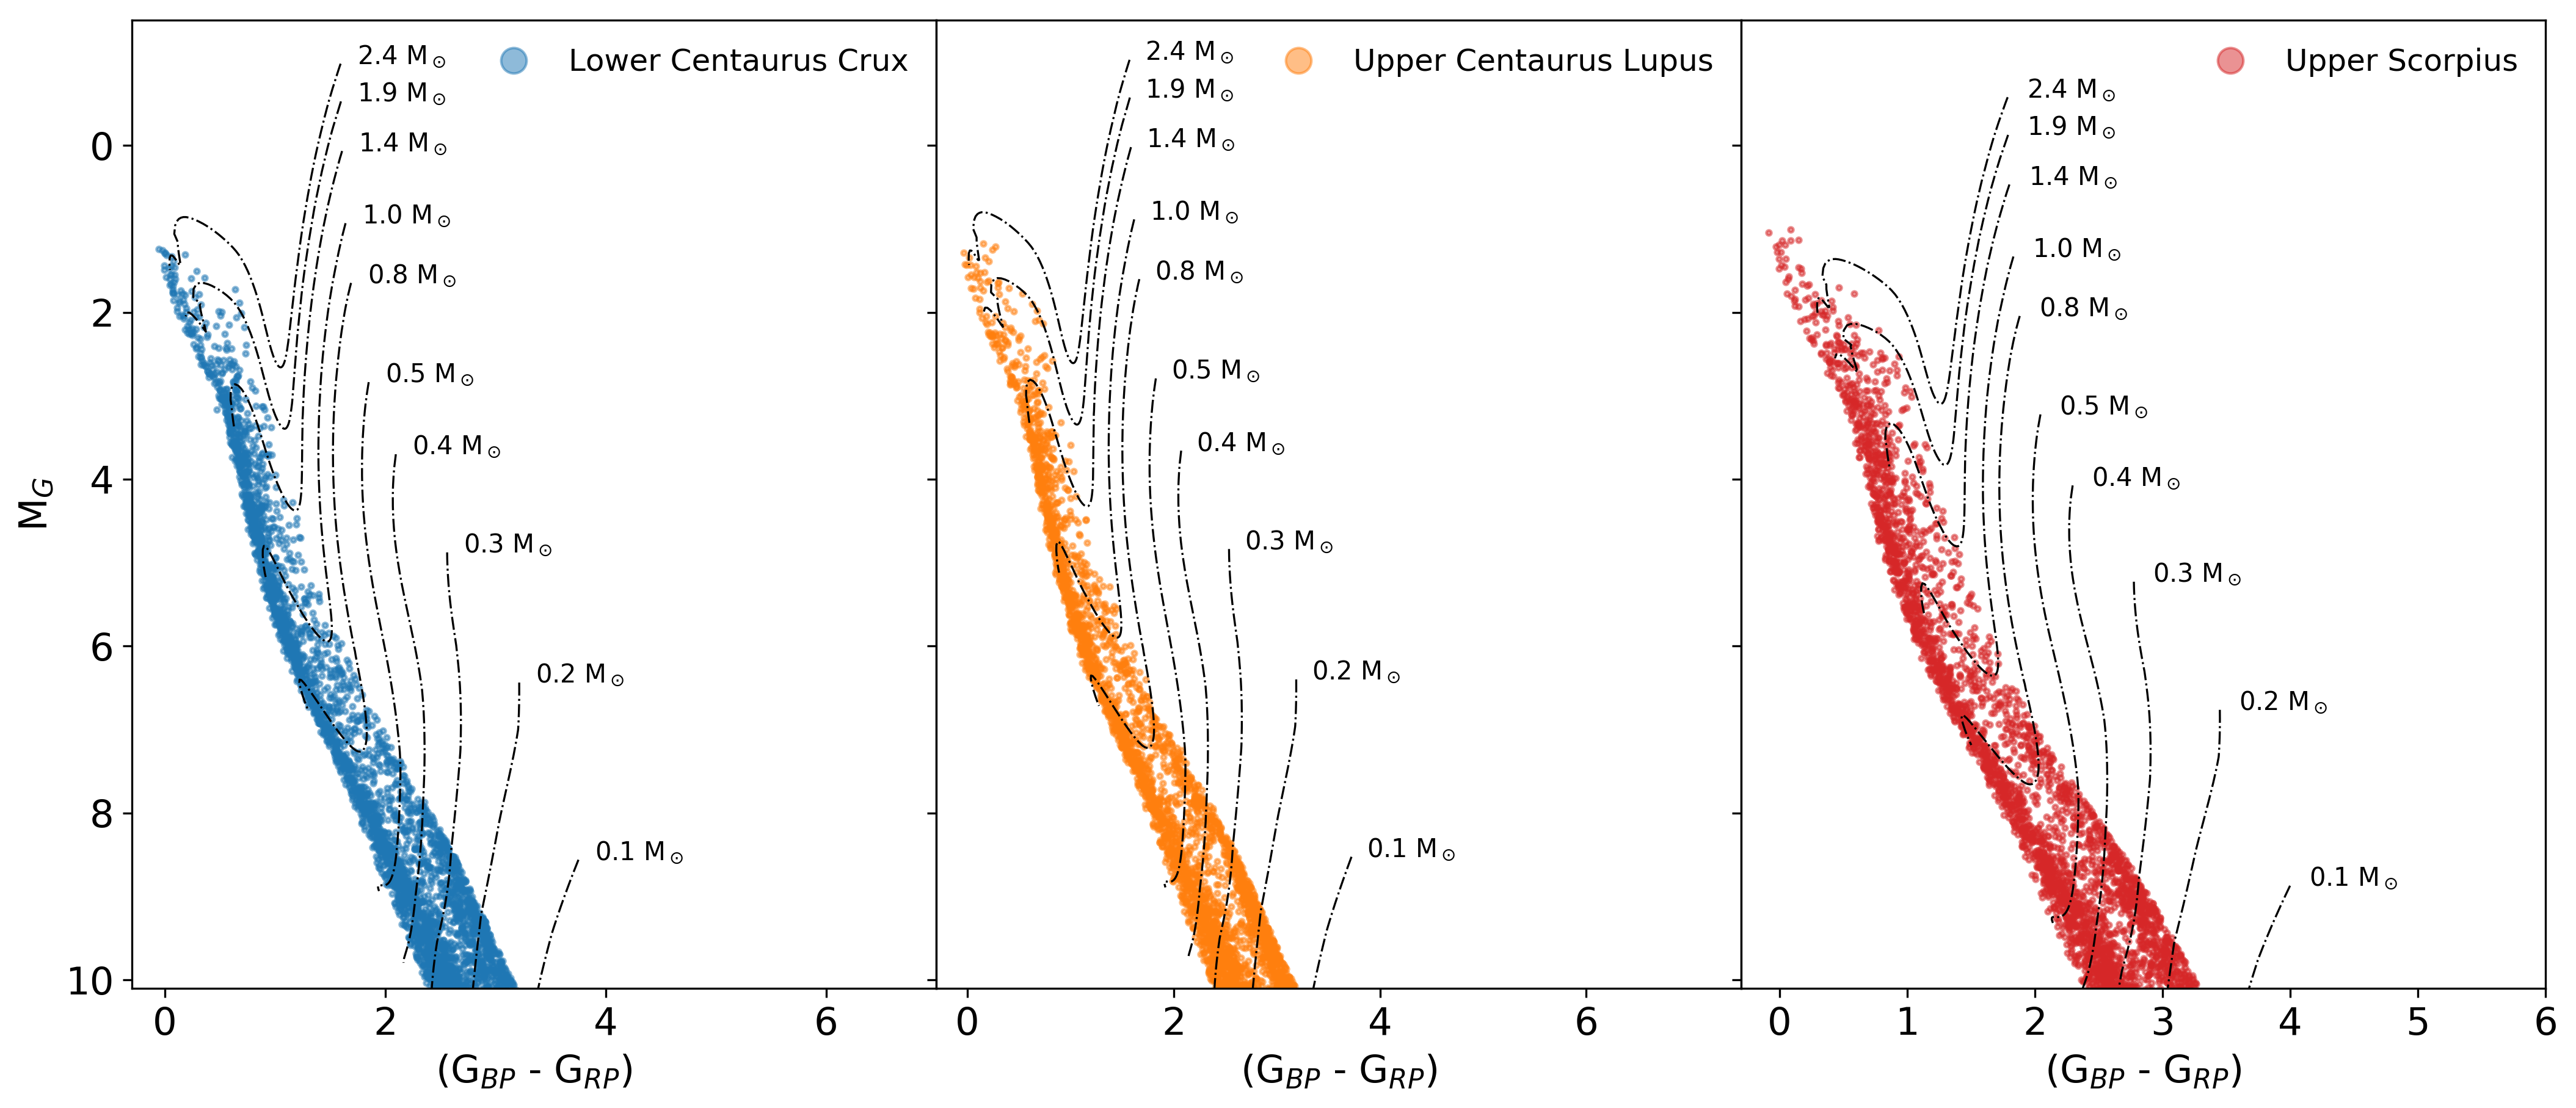
\includegraphics[width = 16cm, height = 7.5cm]{./Graficos/Capitulo_3/7_DR2_LightCurves/CMD_Cleaned_FinalSelection_Tracks.png}} 
\caption{\scriptsize{Color-magnitude diagrams for each subgroup in ScoCen using the filtered out sample, along with stellar tracks using the extinction value proposed by \cauthor{1989A&A...216...44D} (\citeyear{1989A&A...216...44D}). \textit{\textbf{Left}}: LCC stars after cuts are shown in blue. The black lines correspond to different stellar tracks. \textit{\textbf{Center}}: UCL stars after cuts are shown in orange. The black lines correspond to different stellar tracks. \textit{\textbf{Right}}: US stars after cuts are shown in red. The black lines correspond to different stellar tracks. In general for each subgroup, a stellar mass range of $0.1 \textnormal{M}_\odot < \textnormal{M} < 2.4 \textnormal{M}_\odot$ was used to compute the stellar tracks using the \textit{MIST}-package (\cauthor{2016ApJS..222....8D} \citeyear{2016ApJS..222....8D}; \cauthor{2016ApJ...823..102C} \citeyear{2016ApJ...823..102C}). In this case, the extinction values for LCC, UCL, and US correspond to $\textnormal{A}_\textnormal{v} = 0.23$, $\textnormal{A}_\textnormal{v} = 0.17$, and $\textnormal{A}_\textnormal{v} = 0.76$, respectively.}}
\label{fig:DR2_Tracks}
\end{figure}

\begin{figure}[!ht]
\centering
  \subfloat{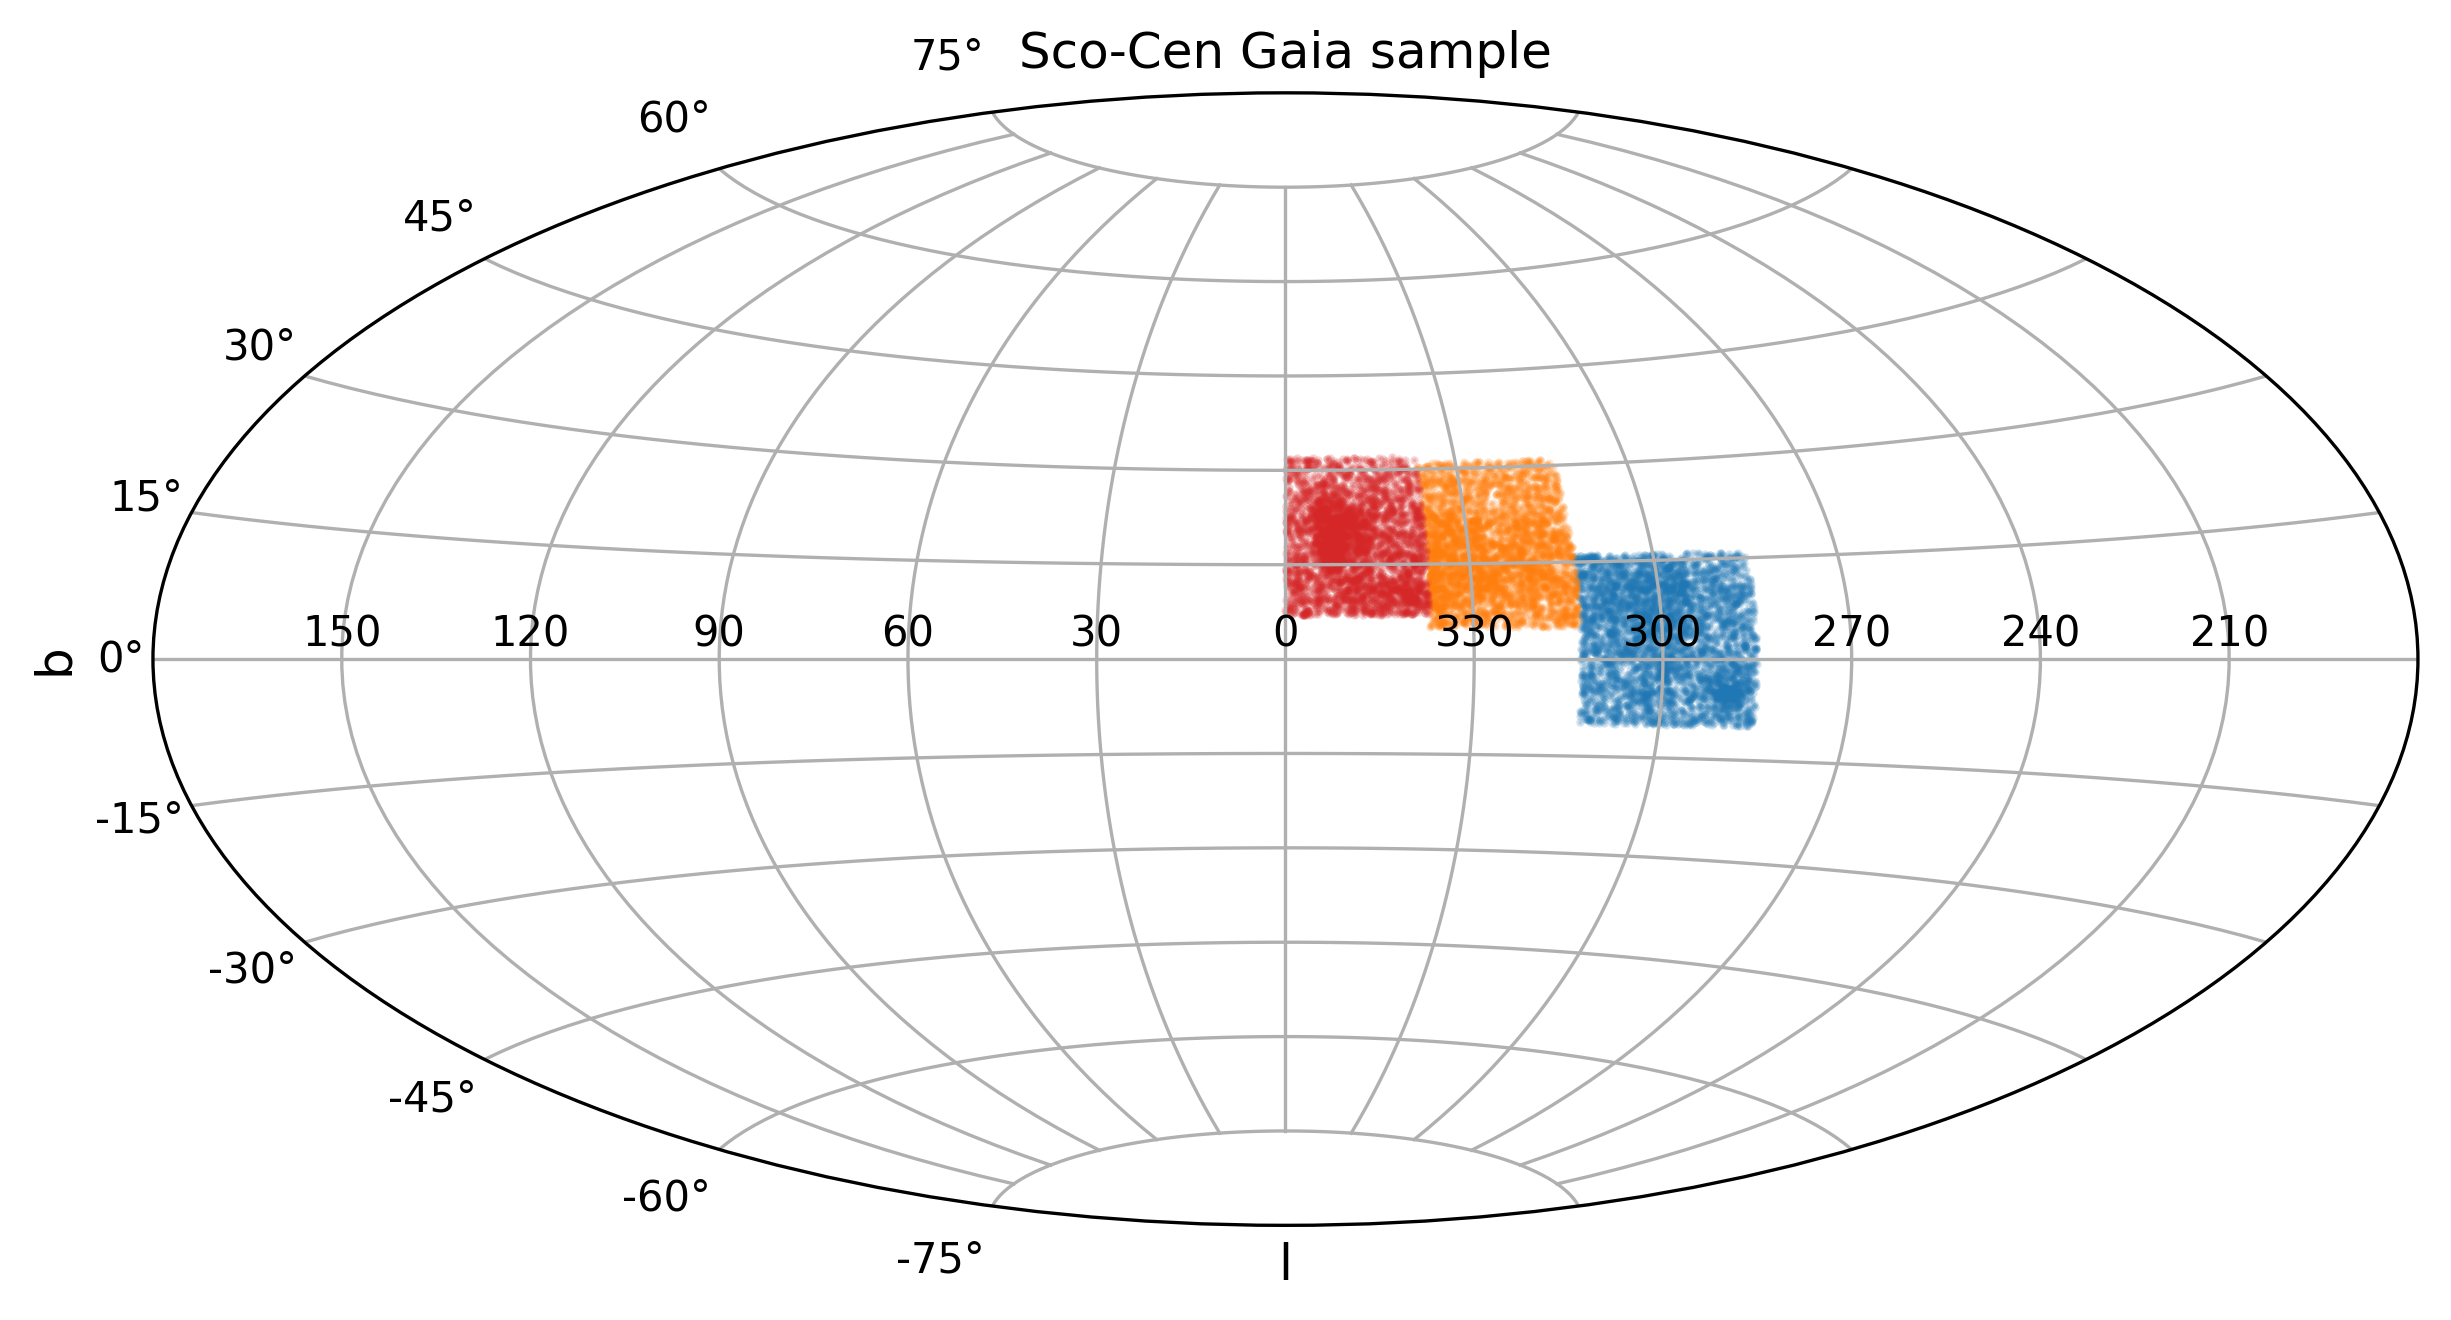
\includegraphics[width = 16cm, height = 8cm]{./Graficos/Capitulo_3/7_DR2_LightCurves/Sco_Cen_FinalSample_Projection.png}} 
\caption{\scriptsize{ScoCen subgroups position in galactic coordinates. Each subgroup LCC (blue), UCL (orange) and US (red), contains the final sample of stars after cleaning \textit{Gaia} DR2 data shown in galactic longitude and galactic latitude. The region covers $\sim 90$-degrees in longitude and $\sim 50$-degrees in latitude.}}
\label{fig:DR2_Projection}
\end{figure}

The final sample and the cross-matching process is addressed in \autoref{sec:LightCurvesSco} and the special case of J1407.

%============================================================================================================================================================

\section{ScoCen Light Curves}\label{sec:LightCurvesSco}

In the last section, we explained the selection process to obtain the final sample of stars in each subgroup of ScoCen using \textit{Gaia} DR2 data. Now, as we want to obtain the light curves available for these stars in the \textit{SuperWASP} database, the next step is to cross-match each object using their coordinates in right ascension and declination. The \href{https://exoplanetarchive.ipac.caltech.edu/cgi-bin/TblSearch/nph-tblSearchInit?app=ExoTbls&config=superwasptimeseries}{SuperWASP-Interface} allows the user to search for an object's light curve using its coordinates including constraints as the start and end of the light curve, the number of data points used in the statistical calculation, the number of points in the actual light curve, the WASP-magnitude, among others. In our particular case, we decided to pass each set of stars in each of the ScoCen subgroups as a list and search for any object within a radius of $0.1~\textnormal{arcsec}$ to ensure that the selected stars correspond to the one measured in \textit{Gaia} DR2. Along with this, the only extra constraint we set was the number of points in the light curve to be greater than $100$ because lots of stars have poor measurements and it is not worthy to retrieve them. Following this steps, we get a final sample of $177$, $1\,053$, and $1\,253$ light curves for LCC, UCL, and US out of the $7\,268$, $6\,244$, and $7\,436$ original sample after all the cuts were applied. It is striking the small number of light curves retrieved for LCC having in mind that for the three subgroups the number of stars is very similar. However, if we observe \autoref{fig:SWASP_DR1_Flux} in \autoref{sec:SWASPdata}, LCC lies close to the mid-plane of the Milky Way where the \textit{SuperWASP} survey is incomplete. In the same way, US happens to have a large number of stars retrieved due to the fact that this subgroup lies in a portion of the night sky which was widely surveyed. The light curves are generated automatically from the data files retrieved for each one of the targets using corrected values of the apparent magnitude as a function the Julian Day.\\

Having said that, we proceed to inspect the light curves possibly showing up features as those reported by \cauthor{2012AJ....143...72M} (\citeyear{2012AJ....143...72M}) for J1407. Our selection criteria retrieve this object in the UCL-subgroup when using the unit weight error cleaning $u$. However, if we apply the $u^2$ criterion then this object is left out of the sample. In spite of that, the method gives us hope in our blind-search for exoplanetary rings. The light curve without averaging the data per night is shown in \autoref{fig:J1407WASPLC}. The dataset corresponds to three different years of observation where the second-year exhibits a remarkable dip. This is the type of features we are interested in because it is the closest report in literature to be a ringed system, thus, we took this as a canonical example for comparison with all the different light curves obtained through the cross-match. Initially, the main scientific aim was to retrieve the light curves and pre-select possible candidates to fit different disks models. However, we decided to just provide a list of interesting light curves showing features as those in J1407 or simply any weird/unexpected variation as inspected by eye. The amount of data is quite large which makes the main goal of the project quite ambitious to achieve in a short time period. Thus, we proposed a final sample of candidates which could be followed up with new observations to complete the light curves that must be averaged per night, so in future works, the final analysis and disk-model fitting can be performed on this sample in order to rule out candidates. The final list of candidates is shown in \autoref{tab:Candidates_Final} where each source has its corresponding \textit{Gaia} DR2 and \textit{SuperWASP} IDs, and right ascension and declination, and the respective error as provided by \textit{Gaia} DR2 data.\\

\begin{figure}[!ht]
\centering
  \subfloat{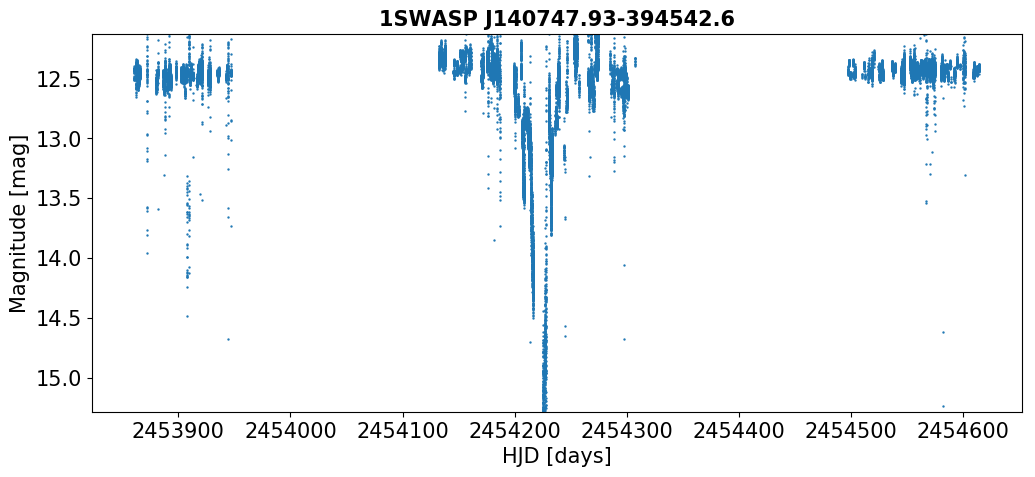
\includegraphics[width = 15cm, height = 7cm]{./Graficos/Capitulo_3/7_DR2_LightCurves/J1407.png}} 
\caption{\scriptsize{1SWASP J$140747.93-394542.6$ (J$1407$) light curve. The figure shows the corrected magnitude as a function of HJD (days) for three different years of observation. A huge dip can be observed during the second-year which is assumed to be produce by a massive system of circumplanetary rings as reported in \cauthor{2012AJ....143...72M} (\citeyear{2012AJ....143...72M}).}}
\label{fig:J1407WASPLC}
\end{figure}

%Candidates 
\begin{table}[]
\centering
\caption{\textit{SuperWASP} candidates cross-matched with \textit{Gaia} DR2.}
\label{tab:Candidates_Final}
\scalebox{0.8}{
\begin{tabular}{llllll}
\hline \textit{Gaia} DR2 ID         & \textit{SuperWASP} ID               & RA {[}deg{]}        & RA\_ERR {[}deg{]} & DEC {[}deg{]}       & DEC\_ERR {[}deg{]}  \\ \hline \hline
 5375292381453195264 & 1SWASP J112917.08-461225.0 & 172.3215  & 0.0499  & -46.2071  &  0.0426  \\
 6107318842082097152 & 1SWASP J134703.99-460848.3 & 206.7665  & 0.0939  & -46.1468  &  0.0617  \\
 6116150703591896064 & 1SWASP J141849.15-394422.5 & 214.7045  & 0.0989  & -39.7397  &  0.1185  \\
 6103779101835413504 & 1SWASP J142352.01-411304.8 & 215.9665  & 0.0533  & -41.2182  &  0.0437  \\
 6098745709402994688 & 1SWASP J143906.15-451537.0 & 219.7756  & 0.0302  & -45.2604  &  0.0378  \\
 6229363700751409152 & 1SWASP J145223.73-244648.9 & 223.0987  & 0.0433  & -24.7804  &  0.0288  \\
 6100760014705034240 & 1SWASP J145302.55-425247.5 & 223.2606  & 0.0387  & -42.8799  &  0.0377  \\
 6198287589442119680 & 1SWASP J145822.27-382555.3 & 224.5929  & 0.0443  & -38.4319  &  0.0454  \\
 6206539802163648512 & 1SWASP J152836.36-334750.3 & 232.1515  & 0.1352  & -33.7974  &  0.0407  \\
 6039361223829141504 & 1SWASP J155606.62-321225.8 & 239.0274  & 0.0189  & -32.2073  &  0.0097  \\
 6042706591035865088 & 1SWASP J160158.04-283057.4 & 240.4919  & 0.0356  & -28.5161  &  0.0159  \\
 6043692028329650176 & 1SWASP J160728.47-254832.8 & 241.8686  & 0.0538  & -25.8091  &  0.0219  \\
 6041822716821447680 & 1SWASP J160826.31-282549.3 & 242.1095  & 0.0422  & -28.4305  &  0.0173  \\
 6043701064940930048 & 1SWASP J160833.29-254010.6 & 242.1386  & 0.0539  & -25.6696  &  0.0253  \\
 6038079708665729024 & 1SWASP J162339.37-294405.6 & 245.9139  & 0.0499  & -29.7349  &  0.0339  \\
 6045393041544132608 & 1SWASP J162452.74-265517.0 & 246.2199  & 0.0593  & -26.9213  &  0.0334  \\ \hline 
\end{tabular}
}
\end{table}

Some light curves show double measurements in different years caused by an object being detected in different cameras and flux not being matched properly. For this reason, we decided to draw the apparent magnitude corrected by \autoref{eq:Mag_Swasp} as a function of HJD as given by \autoref{eq:HJD_Swasp} which helps us to avoid this type of spurious features. However, it is worth noticing that even after correcting the flux (i.e. apparent magnitude) this kind of features are still present for a couple of sources in which we cannot attribute it as a result of bad matching or real measurements. This can be observed in \autoref{fig:SWASP_LightCurve_1} for the second year of observations where the light curve has already been corrected. In \autoref{fig:SWASP_LightCurve_Spurious} and \autoref{fig:SWASP_LightCurve_2}, we present two candidates in order to illustrate how any other light curve looks like in our final sample. It is clear that these light curves do not exhibit dramatic dips as compared to J1407. However, interesting features are present which motivate future work and observations. \autoref{fig:SWASP_LightCurve_2} on the other hand gives the impression of a regular variable star instead of a ringed system around. We decided to keep also this type of light curves because we already have coordinates, parallaxes, and proper motions for all these stars thanks to \textit{Gaia} DR2 which may lead to possible new discoveries.  

\begin{figure}[!ht]
\centering
  \subfloat{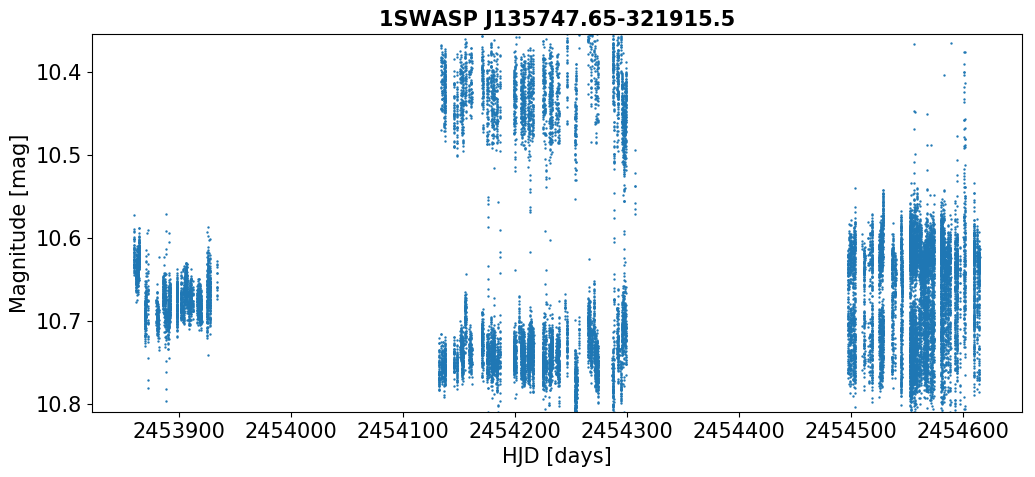
\includegraphics[width = 15cm, height = 7cm]{./Graficos/Capitulo_3/7_DR2_LightCurves/1SWASPJ135747.png}} 
\caption{\scriptsize{1SWASP J$135747.65-321915.5$ light curve. The figure shows the corrected magnitude as a function of HJD (days) for three different years of observation. During the second-year there is a double feature likely to be produced by bad match between different fluxes in different cameras of the \textit{SuperWASP} survey.}}
\label{fig:SWASP_LightCurve_1}
\end{figure}

\begin{figure}[!ht]
\centering
  \subfloat{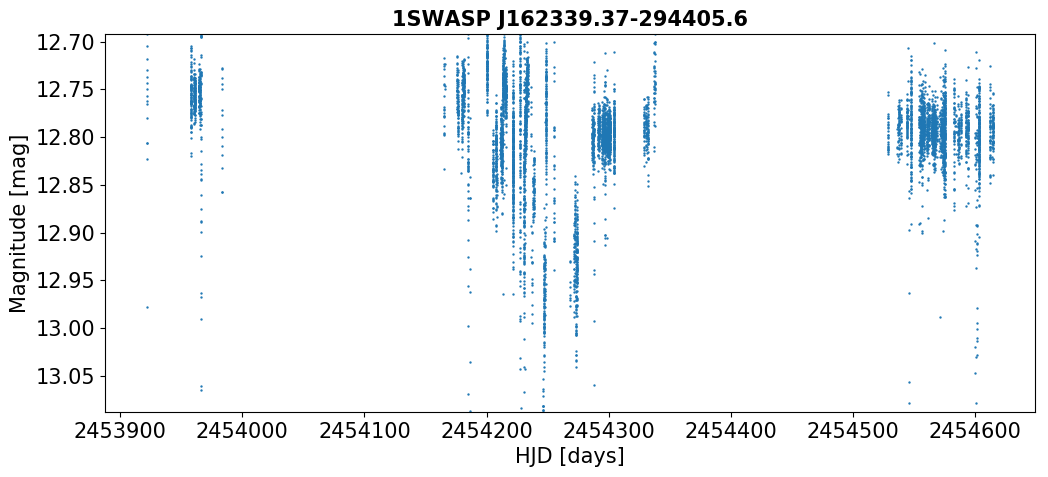
\includegraphics[width = 15cm, height = 7cm]{./Graficos/Capitulo_3/7_DR2_LightCurves/1SWASP_J162339.png}} 
\caption{\scriptsize{1SWASP J$162339.37-294405.6$ light curve. The figure shows the corrected magnitude as a function of HJD (days) for three different years of observation. During the second-year there is a feature that reminds the observations of J1407 in $2012$.}}
\label{fig:SWASP_LightCurve_Spurious}
\end{figure}

\begin{figure}[!ht]
\centering
  \subfloat{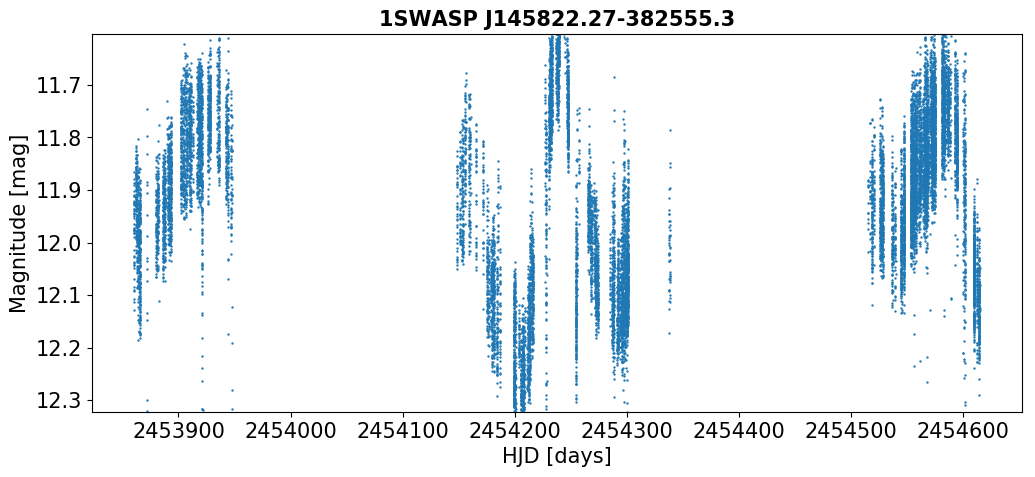
\includegraphics[width = 15cm, height = 7cm]{./Graficos/Capitulo_3/7_DR2_LightCurves/1SWASP_J145822.png}} 
\caption{\scriptsize{1SWASP J$145822.27-382555.3$ light curve. The figure shows the corrected magnitude as a function of HJD (days) for three different years of observation. The light curve presents a variations that gives the sensation of a sinusoidal curve. Day average and model fitting are needed to give a final verdict.}}
\label{fig:SWASP_LightCurve_2}
\end{figure}

%\subsection{J1407 light curve}\label{subsec:LightCurvesSco_1}

%============================================================================================================================================================

\section{ScoCen Pre-Main Sequence Population}
%\cauthor{} \citeyear{}

In different works as those by (\cauthor{1999AJ....117..354D} \citeyear{1999AJ....117..354D}; \cauthor{2018MNRAS.tmp..210W} \citeyear{2018MNRAS.tmp..210W}) kinematic analysis from proper motions and radial velocities has been essential to study OB associations as ScoCen in order to separate members from the foreground and background stellar population. Spectroscopic and photometric surveys usually lack low-mass pre-main sequence stars creating a bias towards more massive members. In 2017 \cauthor{Zari17} (\citeyear{Zari17}) used \textit{Gaia} DR1 data to isolate the pre-main sequence population in the Orion region using the apparent magnitude versus color and combining also \textit{2MASS} photometry. On the other hand \cauthor{Skrutskie06} (\citeyear{Skrutskie06}) also addressed the same problem but using \textit{Gaia} DR2 data and constructing the Hertzsprung-Russell in which the pre-main sequence population is more precisely isolated. In our case, we decided to apply the same method but to the ScoCen region because this provides an easy way to pre-select member of the association and search for probably hidden features.\\

In the first place, we extended the original three boxes which limit the \textit{Scorpius-Lupus-Centaurus-Crux} area on the sky \cauthor{Blaauw46} (\citeyear{Blaauw46}). The new limits contain the original three boxes and correspond to all stars with galactic coordinates $285^\circ\leq\ell\leq360^\circ$ and $-10^\circ\leq b\leq+32^\circ$. This is shown in the right panel of \autoref{fig:ScoOB_premain} in which the color map stands for the logarithmic number of stars in hexagon bins. Additionally, the new range of parallax was set to lie between $5$ and $12$ mas to cover a wider volume in space. No cuts in right ascension and declination proper motions or total proper motion were used just to leave the sample as free as possible of constraints known in the literature due to the fact that if the method of pre-selecting the pre-main sequence is powerful enough, then the overall features of the OB association will pop up naturally. Sources with spurious parallaxes and bad photometry were cleaned following the same method explained in \autoref{sec:CleaningProcess} as proposed in \cauthor{2018arXiv180409366L} (\citeyear{2018arXiv180409366L}). The first sample contains $134\,587$ source, however, after the selection process our sample is made up of $120\,911$ sources represented as blue dots in the left of \autoref{fig:ScoOB_premain} which corresponds to the Hertzsprung-Russell diagram. It is worth noticing that the pre-main sequence and main-sequence populations are well separated for $(G_\mathrm{BP}-G_\mathrm{RP})>1$, where at $(G_\mathrm{BP}-G_\mathrm{RP})>2$ the separation is well above the $0.75$ magnitude expected from a population of equal mass binaries. Thus, we proceeded to select the young population in our sample using an interactive selection method which allows us to draw a polygon around the region of study and then retrieve the information associated to sources inside the polygon. The polygon and notebooks are available at Zenodo, \href{https://zenodo.org/record/1286576#.Wx6NAmMzaV4}{doi:10.5281/zenodo.1286576}.\\ 

\begin{figure}[!ht]
\centering
  \subfloat{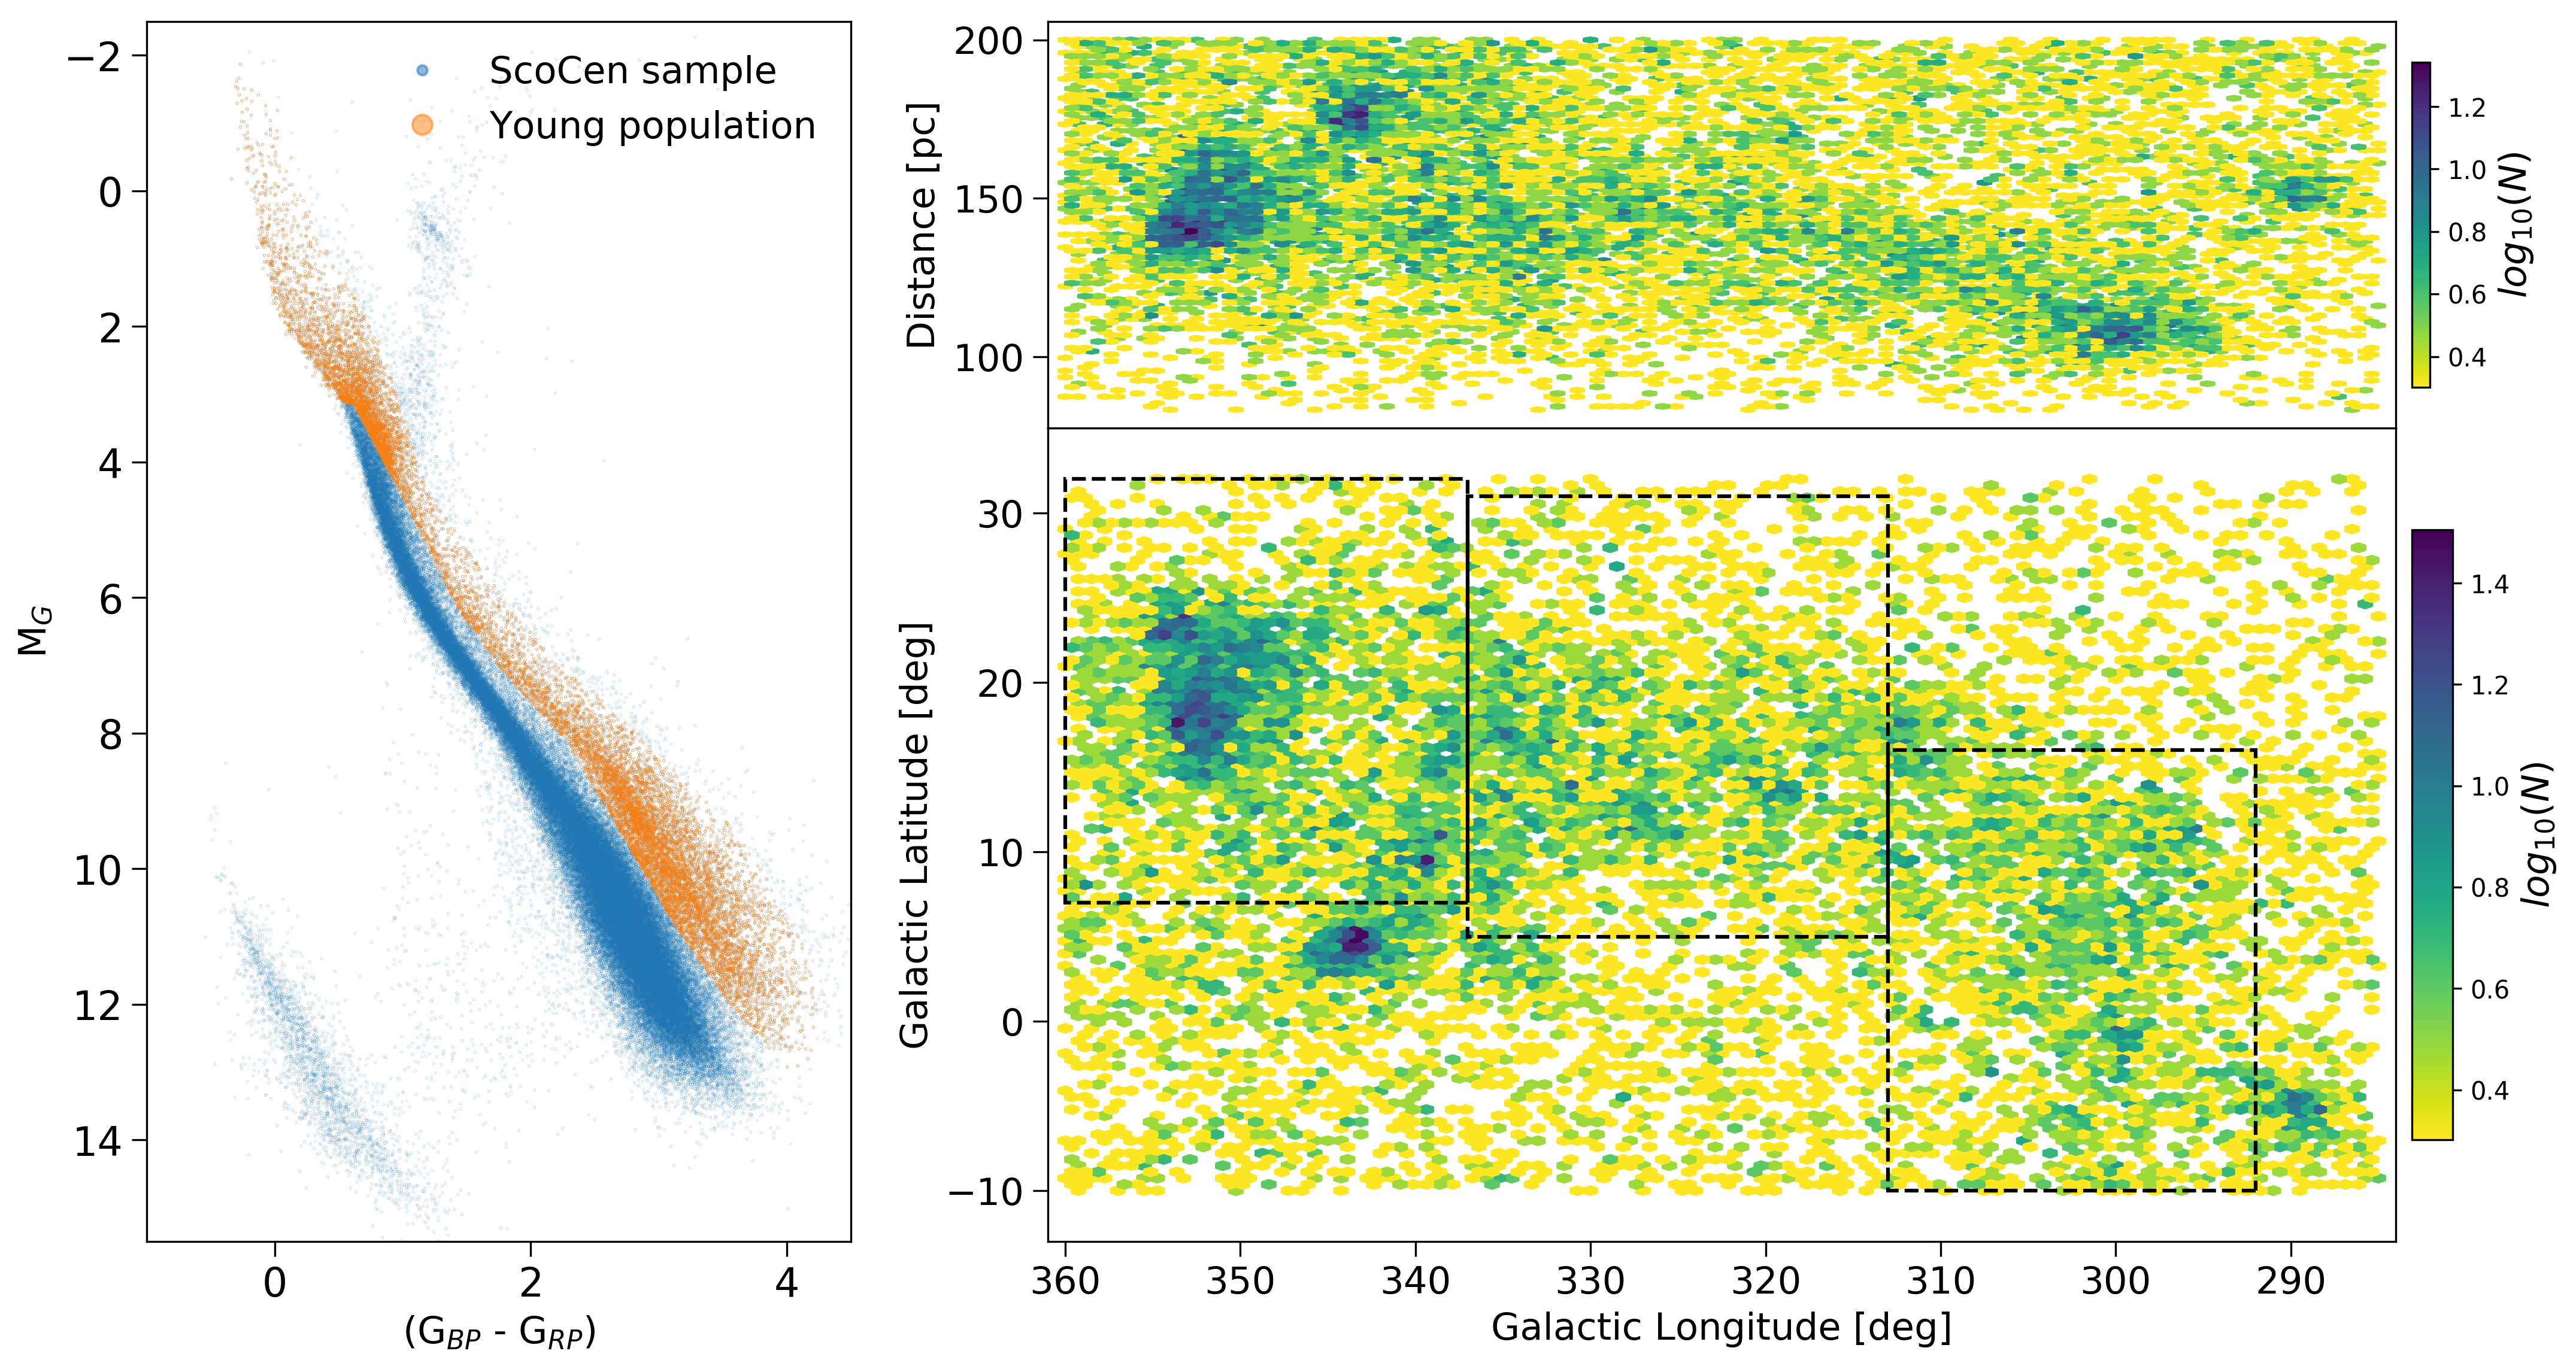
\includegraphics[width = 16cm, height = 8.5cm]{./Graficos/Capitulo_3/ScoCen_Coordinates.png}} 
\caption{\scriptsize{Color-magnitude diagram of the ScoCen region. The orange dots represent the young population selected (pre-main sequence stars) while the blue dots represents the whole sample after the cleaning process. \textit{\textbf{Bottom right:}} Sky distribution of the young stellar population. The classical boundaries of the three subgroups of ScoCen (from left to right, \textit{Upper Scorpius}, \textit{Upper Centaurus-Lupus}, and \textit{Lower Centaurus-Crux}), as defined in \cauthor{1999AJ....117..354D} (\citeyear{1999AJ....117..354D}), are indicated. \textit{\textbf{Top right:}} Distance distribution (with distance calculated as $1/\varpi$) as a function of Galactic longitude.}}
\label{fig:ScoOB_premain}
\end{figure}

In general, in \autoref{fig:ScoOB_premain} a clear concentration of pre-main sequence stars is evident following the original three-boxes region, consistent with most of the selected sources being association members. The LCC and UCL subgroups show a clear concentration of stars but relatively sparse in comparison to US which shows a remarkable high-density concentration of the selected young population. The expanded search reveals a notorious over-density out of the US original box-limits associated with ScoCen ($b\sim5^\circ$ and $\ell\sim345^\circ$) at a mean distance of $\sim180\mathrm{pc}$ ($5$-$6$~mas) (see \autoref{fig:ScoOB_premain} top-right panel). This feature was previously noted by \cauthor{1999AJ....117..354D} (\citeyear{1999AJ....117..354D}) (see their Section 4.5 and Figure 9), and in \cauthor{2016MNRAS.461..794P} (\citeyear{2016MNRAS.461..794P}) using \textit{Gaia} DR1 data. However, our sample contains more sources exposing this region with better clarity allowing new works following the kinematics analysis to have a higher chance of finding new stars which could belong to the OB association much more easily. There is also a concentration of sources near $(\ell,b)=(290^\circ,-5^\circ)$ which corresponds to the well-known IC 2602 cluster lying at $\varpi = 6.74 \pm 0.25$~mas as reported by (\cauthor{vanLeeuwen17} \citeyear{vanLeeuwen17}). Thus, in overall, the resulting maps of the pre-main sequence population can be used to guide more detailed membership studies of OB associations, including a thorough re-assessment of the traditional association and subgroup boundaries. We anticipate a major revision in our knowledge of OB associations coupled with new insights into the triggering and propagation of star formation.\\

Summing up, it turns out to be quite useful to use \textit{Gaia} DR2 data in order to retrieve sources of a volume-limited sample in parallax and coordinates to lately build up the Hertzsprung-Russell diagram and select the young population or pre-main sequence stars. Using this one can visualize the overall shape of the associations and different over-densities possibly associated with them. After that, different analysis as the classical kinematic approach can be used to finely select those sources that actually belong to the same association.  